% ------------------------------------------------------------------------
% ------------------------------------------------------------------------
% abnTeX2: Modelo de Trabalho Academico (tese de doutorado, dissertacao de
% mestrado e trabalhos monograficos em geral) em conformidade com 
% ABNT NBR 14724:2011: Informacao e documentacao - Trabalhos academicos -
% Apresentacao
% ------------------------------------------------------------------------
% ------------------------------------------------------------------------

% ------------------------------------------------------------------------
% ------------------------------------------------------------------------
% abnTeX2: Modelo de Trabalho Academico (tese de doutorado, dissertacao de
% mestrado e trabalhos monograficos em geral) em conformidade com 
% ABNT NBR 14724:2011: Informacao e documentacao - Trabalhos academicos -
% Apresentacao
% ------------------------------------------------------------------------
% ------------------------------------------------------------------------

\documentclass[
	% -- opções da classe memoir --
	12pt,				% tamanho da fonte
	% openright,			% capítulos começam em pág ímpar (insere página vazia caso preciso)
	% twoside,			% para impressão em verso e anverso. Oposto a oneside
	a4paper,			% tamanho do papel. 
	% -- opções da classe abntex2 --
	%chapter=TITLE,		% títulos de capítulos convertidos em letras maiúsculas
	%section=TITLE,		% títulos de seções convertidos em letras maiúsculas
	%subsection=TITLE,	% títulos de subseções convertidos em letras maiúsculas
	%subsubsection=TITLE,% títulos de subsubseções convertidos em letras maiúsculas
	% -- opções do pacote babel --
	english,			% idioma adicional para hifenização
	% french,				% idioma adicional para hifenização
	spanish,			% idioma adicional para hifenização
	brazil				% o último idioma é o principal do documento
	]{abntex2}

	% ---
	% Pacotes básicos 
	% ---
	\usepackage{lmodern}			% Usa a fonte Latin Modern			
	\usepackage[T1]{fontenc}		% Selecao de codigos de fonte.
	\usepackage[utf8]{inputenc}		% Codificacao do documento (conversão automática dos acentos)
	\usepackage{lastpage}			% Usado pela Ficha catalográfica
	\usepackage{indentfirst}		% Indenta o primeiro parágrafo de cada seção.
	\usepackage{color}				% Controle das cores
	\usepackage{graphicx}			% Inclusão de gráficos
	\usepackage{microtype} 			% para melhorias de justificação
	\usepackage{epsfig,psfrag,amsmath,tabularx} % para figuras eps e simbolos matematicos
% ---

% ---
% Pacotes de citações
% ---
\usepackage[brazilian,hyperpageref]{backref}	 % Paginas com as citações na bibl
\usepackage[alf]{abntex2cite}					 % Citações padrão ABNT

% --- 
% CONFIGURAÇÕES DE PACOTES 
% --- 

% ---
% Configuracoes do pacote backref
% Usado sem a opcao hyperpageref de backref
\renewcommand{\backrefpagesname}{Citado na(s) página(s):~}
% Texto padrao antes do numero das paginas
\renewcommand{\backref}{}
% Define os textos da citacao
\renewcommand*{\backrefalt}[4]{
	\ifcase #1 %
		Nenhuma citação no texto.%
	\or
		Citado na página #2.%
	\else
		Citado #1 vezes nas páginas #2.%
	\fi}%
% ---

% ---
% Pacotes definidos pelo autor
% Pacotes inseridos pelo autor OJF
\usepackage[table]{xcolor}
\usepackage[linesnumbered,ruled,portuguese]{algorithm2e} % by OJF
 \usepackage{multirow}
\usepackage{longtable}
\usepackage{pdflscape}
\usepackage{amssymb}


% \usepackage{subfigure}
% \usepackage{cleveref}
% \usepackage{subfig}
% \usepackage[subfigure]{tocloft}
 \usepackage{tocloft}

\let\cleardoublepage\clearpage
% ---
% Espacos H2, Hoo, L2, Loo
\newcommand\Hi{{\mathcal{H}}_{\infty}}
\newcommand\Hd{{\mathcal{H}}_{2}}
\newcommand\Li{{\mathcal{L}}_{\infty}}
\newcommand\Ld{{\mathcal{L}}_{2}}


\def\reais{{\rm I\kern-.17em R}} % R de reais
\def\Dest{{\rm I\kern-.17em D}} % R de reais
\newcommand{\Dgest}{\ensuremath{\mathcal{D}}}
\newcommand{\naturais}{\mathbb{N}}
\newcommand{\inteiros}{\mathbb{Z}_{+}}
\newcommand{\matlab}{{\sc Matlab}}

%super parenteses
\makeatletter
\def\Biggg#1{{\hbox{$\left#1\vbox to29\p@{}\right.\n@space$}}}
\newdimen\bracketwidth
\settowidth{\bracketwidth}{\Biggg(} \makeatother


%\newcommand{\carinha}{\raisebox{-.2ex}{\epsfxsize 3mm \epsffile{cara.eps}}}

% Bolds
\newcommand{\I}{{\bf I}}
\newcommand{\Z}{{\bf 0}}
\newcommand{\Bfres}{\mathcal{B}}

% funcoes
\newcommand{\Tr}{\mbox{Tr}}

% Referencia com parenteses
\newcommand{\bref}[1]{\mbox{(\ref{#1})}}

% Ambiente de equacoes
\newcommand\be{\begin{equation}}
\newcommand\ee{\end{equation}}
\newcommand\vi{\vspace{\baselineskip}}

% newtheorems e similares

\newtheorem{teorema}{\noindent{\bf Teorema} }[chapter]
\newtheorem{lema}{\noindent{\bf Lema} }[chapter]
\newtheorem{corolario}{\noindent{\bf Corolário} }[chapter]
\newenvironment{prova}{\noindent{\bf Prova:}}{\null\hfill $\rule{1.5mm}{1.5mm}$}
\newtheorem{definicao}{\noindent{\bf Definição} }[chapter]

\newcommand{\simplex}{\Delta_N}



\newcommand{\Aal}{A(\alpha)}
\newcommand{\Bal}{B(\alpha)}
\newcommand{\Cal}{C(\alpha)}
\newcommand{\Dal}{D(\alpha)}


\newcommand{\Pal}{P(\alpha)}
\newcommand{\Gal}{G(\alpha)}
\newcommand{\Hal}{H(\alpha)}
\newcommand{\Qal}{Q(\alpha)}
\newcommand{\Xal}{X(\alpha)}
\newcommand{\Xual}{X_1(\alpha)}
\newcommand{\Xdal}{X_2(\alpha)}

\newcommand{\Sfr}{\mathcal{S}}

\newcommand{\Xfal}{\mathcal{X}(\alpha)}
\newcommand{\Bfal}{\mathcal{B}(\alpha)}
\newcommand{\Qfal}{\mathcal{Q}(\alpha)}
\newcommand{\Sfal}{\mathcal{S}(\alpha)}

\newcommand{\Kfr}{\mathcal{K}}
\newcommand{\Ifr}{\mathcal{I}}
\newcommand{\Afr}{\mathcal{A}}
\newcommand{\Pfr}{\mathcal{P}}
\newcommand{\Cfr}{\mathcal{C}}
\newcommand{\Gfr}{\mathcal{G}}
		% arquivo com possiveis macros definidas pelo autor
% ---

% ---
% Informacoes de dados para CAPA e FOLHA DE ROSTO
% ---



% \titulo{Aplicação de técnicas de Recuperação de Informação para Organização e Extração de Históricos de Decisões de Documentos de Reuniões}
\titulo{Avaliação de técnicas de Recuperação de Informação para Organização e Extração de Conhecimento de Documentos de Reuniões}
\autor{Ovídio José Francisco\footnote{E-mail: \texttt{ovidiojf@gmail.com} | Lattes: \url{http://lattes.cnpq.br/6601215787925926}}}
\local{Sorocaba, SP}
\data{\today}
\orientador{Prof.ª Dr. Katti Faceli}
\coorientador{Prof. Dr. Rafael Geraldeli Rossi}
\instituicao{%
  Universidade Federal de São Carlos -- UFSCar
  \par
  Centro de Ciências em Gestão e Tecnologia -- CCGT
  \par
  Programa de Pós-Graduação em Ciência da Computação -- PPGCC-So}
\tipotrabalho{Dissertação (Mestrado)}
% O preambulo deve conter o tipo do trabalho, o objetivo, 
% o nome da instituicao e a Area de concentracao 
\preambulo{Dissertação de mestrado apresentada ao Programa de Pós-Graduação em Ciência da Computação (PPGCC-So) da Universidade Federal de São Carlos como parte dos requisitos exigidos para a obtenção do título de Mestre em Ciência da Computação. Linha de pesquisa: Aprendizado de Máquina.}
% ---


% ---
% Configuracoes de aparencia do PDF final

% alterando o aspecto da cor azul
\definecolor{blue}{RGB}{41,5,195}

% informacoes do PDF
\makeatletter
\hypersetup{
     	%pagebackref=true,
		pdftitle={\@title}, 
		pdfauthor={\@author},
    	pdfsubject={\imprimirpreambulo},
	    pdfcreator={LaTeX with abnTeX2},
		pdfkeywords={abnt}{latex}{abntex}{abntex2}{trabalho acadêmico}, 
		colorlinks=true,       		% false: boxed links; true: colored links
    	linkcolor=blue,          	% color of internal links
    	citecolor=blue,        		% color of links to bibliography
    	filecolor=magenta,      		% color of file links
		urlcolor=blue,
		bookmarksdepth=4
}
\makeatother
% --- 

% --- 
% Espacamentos entre linhas e paragrafos 
% --- 

% O tamanho do paragrafo é dado por:
\setlength{\parindent}{1.3cm}

% Controle do espaçamento entre um parágrafo e outro:
\setlength{\parskip}{0.2cm}  % tente também \onelineskip

% ---
% compila o indice
% ---
\makeindex
% ---




% ----
% Inicio da dissertacao
% ----
\begin{document}

% Retira espaco extra obsoleto entre as frases.
\frenchspacing


% ----------------------------------------------------------
% ELEMENTOS PRE-TEXTUAIS
% ----------------------------------------------------------
% \pretextual

% ---
% Capa
% ---
\imprimircapa
% ---

% ---
% Folha de rosto
% (o * indica que havera a ficha bibliografica)
% ---
\imprimirfolhaderosto*
% ---

% ---
% Inserir a ficha bibliografica
% ---
% % Este é um exemplo de Ficha Catalografica, ou ``Dados internacionais de
% catalogacao-na-publicacao''. Voce pode utilizar este modelo como referencia. 
% Porem, a biblioteca da universidade irá lhe fornecer um PDF
% com a ficha catalografica definitiva apos a defesa do trabalho. Quando estiver
% com o documento, salve-o como PDF no diretorio do seu projeto e substitua todo
% o conteudo de implementacao deste arquivo pelo comando abaixo:
%
% \begin{fichacatalografica}
%     \includepdf{fig_fichaCatalografica.pdf}
% \end{fichacatalografica}

\begin{fichacatalografica}
	\vspace*{\fill}					% Posicao vertical
	\hrule							% Linha horizontal
	\begin{center}					% Minipage Centralizado
	\begin{minipage}[c]{12.5cm}		% Largura
	
	<<Sobrenome>>, <<Nome do aluno>> %Substituir pelos seus dados. Exemplo: Silva, Pedro da
	
	\hspace{0.5cm} \imprimirtitulo  / \imprimirautor. --
	\the\year.
	
	\hspace{0.5cm} \pageref{LastPage} f. : 30 cm.\\
	
	\hspace{0.5cm}
	\parbox[t]{\textwidth}{\imprimirtipotrabalho~--~\imprimirinstituicao.\\ \imprimirorientadorRotulo~\imprimirorientador\\
	Banca examinadora: \imprimirorientador, Prof. Dr. <<Membro 1>>, Prof. Dr. <<Membro 2>>\\
	Bibliografia}\\

	\vspace{0.5cm}
	\hspace{0.5cm}
		1. <<Palavra-chave1>>. % Substituir
		2. <<Palavra-chave2>>. % Substituir
		3. <<Palavra-chave3>>. % Substituir
		I. Orientador.
		II. Universidade Federal de S\~{a}o Carlos.
		III. Título\\ 			
	
	
	\end{minipage}
	\end{center}
	\hrule
\end{fichacatalografica}
% ---
% ---

% ---
% Inserir folha de aprovacao
% ---
% % Este é um exemplo de Folha de aprovacao, elemento obrigatorio da NBR
% 14724/2011 (secao 4.2.1.3). Voce pode utilizar este modelo ate a aprovacao
% do trabalho. Apos isso, substitua todo o conteudo deste arquivo por uma
% imagem da pagina assinada pela banca com o comando abaixo:
%
% \includepdf{folhaAprovacao_final.pdf}
%
\begin{folhadeaprovacao}

\vspace*{\fill}

\begin{center}
\LARGE\textbf{<<COLOQUE AQUI A CÓPIA DA\\FOLHA DE APROVAÇÃO ASSINADA>>}
\end{center}

\vspace*{\fill}
  
\end{folhadeaprovacao}
% ---

% ---
% Dedicatoria
% ---
%======================================== Dedicatoria =========================================
\begin{dedicatoria}
   \vspace*{\fill}
   \centering
   \noindent
   % \textit{ Coloque a sua dedicatória aqui;\\
   % Coloque a sua dedicatória aqui.}
   \vspace*{\fill}
\end{dedicatoria}
%==============================================================================================

% ---

% ---
% Agradecimentos
% ---
%======================================= Agradecimentos =======================================
\begin{agradecimentos}

	\noindent Agradeço,\\[2mm]
	ao xxxxxxx por yyyyyyy.\\[2mm]
	ao xxxxxxx por yyyyyyy.

\end{agradecimentos}
%==============================================================================================

% ---

% ---
% Epigrafe
% ---
%======================================== Epigrafe ===================================
\begin{epigrafe}
    \vspace*{\fill}
	\begin{flushright}
		\textit{``Não há relação de poder sem constituição \\
			correlata de um campo de saber, nem saber \\
		que não suponha e não constitua ao mesmo \\ tempo relações de poder'' \\ (Foucault)}

		% toda forma de saber produz poder
	\end{flushright}
\end{epigrafe}
%==============================================================================================

% ---

% ---
% RESUMOS
% ---
%================================= Resumo e Abstract ========================================
\setlength{\absparsep}{18pt} % ajusta o espaçamento dos paragrafos do resumo 
                     
% --- 
% resumo em português
% --- 
\begin{resumo}

Em um contexto em que a grande parte das informações armazenadas pelas organizações está em formato textual, o desenvolvimento de ferramentas computacionais para extração e organização automática dessas informações é uma tarefa que retém atenção e relevância.
%
Os modelos de extração de tópicos são recorrentemente empregados nessa tarefa. Esses modelos são capazes de estabelecer relações e encontrar padrões latentes em coleções de documentos textuais.
%
No entanto, há um desafio adicional em documentos constituídos por múltiplos assuntos. Para textos onde há transição de assuntos faz-se necessário, em primeiro lugar, encontrar porções de texto que tratam de um único assunto. Para isso, as técnicas de Segmentação Textual são utilizada para dividir um texto em segmentos com um assunto relativamente independente.
%
%
%
%
%
% Criação de estrutura. 
O uso combinado de algoritmos de Segmentação Textual e Extração de Tópicos pode então ser aplicado para criar uma estrutura que ajuda a entender os dados textuais, os quais são inerentemente não estruturados.
% 
A criação de uma estrutura organizada em tópicos, que incorpora informações latentes sobre o \textit{corpus} favorece técnicas de Recuperação de Informação. Essa abordagem permite a expansão do espaço de busca além do conjunto de termos original de cada segmento, e a identificação de trechos mais relevantes à consulta.
% 
Nesse trabalho, é apresentada uma metodologia para conectar as técnicas de Segmentação Textual aos modelos de Extração de tópicos a fim de gerar uma estrutura derivada de um \textit{corpus} não estruturado, a qual concentra os textos originais acrescidos de informações latentes e organizadas por sua semelhança semântica.
% 
% 
% 
% 
% 
% 
A pesquisa desse trabalho de mestrado investigou as técnicas de Segmentação Textual e Extração de Tópicos para o desenvolvimento de um sistema de Recuperação de Informação em uma coleção de atas de reunião. 
% 
Desenvolveu-se uma sistema para entregar ao usuário os segmentos mais relevantes à consulta. Os trechos exibidos são agrupados por tópicos, o que também possibilita consultas exploratórias à base dados, por meio da navegação por grupos de segmentos relacionados semanticamente. Além disso, trechos pouco relevantes são omitidos, permitindo resultados concentrados no assunto pesquisado.
% 
% 
% 
% 
Foram avaliados cinco técnicas de Segmentação Textual e três modelos de Extração de Tópicos da literatura. Com base no conjunto de atas estudado, criou-se um \textit{corpus} anotado manualmente com informações sobre a composição temática das atas e as transições entre os assuntos. O \textit{corpus} anotado serviu como referência para avaliação objetiva das técnicas de Segmentação Textual. Avaliou-se ainda, os resultados obtidos com os modelos de Extração Tópicos junto a profissionais ligados ao contexto de atas de reunião.
% 
% 
% 
% 
Os resultados sugerem que as técnicas utilizadas e a metodologia apresentada entregam respostas satisfatórios. Contudo, mais dados podem ser necessários para execução de novos experimentos a fim de aprimorar as técnicas utilizadas.
% 
% 
% 
% 
% 
A implementação do sistema e das ferramentas utilizadas para esse trabalho, bem como os resultados obtidos nas avaliações, juntamente com o \textit{corpus} anotado, são as principais contribuições desse trabalho no intuito de dar aportes ao desenvolvimento de novos trabalhos.
% 
% 
% 
% 
% 
% criação de um copus anotado mais robusto e 
% bem como avaliações das técnicas utilizadas bem implementação das ferramentas implementadas. 


\textbf{Palavras-chaves}: 
Recuperação de informação. 
Segmentação textual. 
Extração de tópicos.
Atas de reunião.

\end{resumo}
% --- 


% --- 
% resumo em ingl�s
% --- 
\begin{resumo}[Abstract]
 \begin{otherlanguage*}{english}




In a context where the most informations stored by the organizations is in the text format, the development of computer tools for automatic extraction and organization of this information is a task that holds attention and relevance.
%
The extraction topic models are often employed in this task. This models are able  to establish relations between documents and found latents patterns in sets of them.  
However, there is an additional challenge for documents composed by multiples subjects. For texts with subject shifts, it is necessary, in fist, found the chunks of texts that address a single subject. So, the Text Segmentation techniques are used to break a text in segments with a relatively independent issue.  
The combination of the Text Segmentation and Topic Extraction algorithms, can be used to make an structure that helps to understanding textual data, which are inherently non structured.  
The creation of an topic organized structure, that incorporates latent information concerning the \textit{corpus}, favors Information Retrievals techniques. This approach allows query expansion space, besides the original set of terms of each segment, and the identification most relevant pieces of text.  
This work presents an methodology to connect the Text Segmentation techniques to the Topic Extraction Models, in order to generates an derivative structure from a non structured \textit{corpus}, which concentrates the original texts plus the latent informations and organized by semantic likeness.  
The research for this thesis investigates the Text Segmentation techniques and the Topic Extraction Models to develop an Information Retrieval system for meeting minutes.  
We develops an system to give to the user the most relevant segments to the query. The segmentos presented are clustered by this topics, that also enables exploratory searches to the data base, through browsing by groups of semantically related segments. Furthermore, less relevant segments are omitted, allowing results focused on the researched subject.  
Five techniques of Text Segmentation and three Topic Extraction models from the literature was evaluated. Based on the set of meeting minutes analysed, we create an manually annotated \textit{corpus} with informations on the thematic composition of the meeting minutes and about the issue shifts. The annotated \textit{corpus} served as reference to objective evaluation of the Text Segmentation techniques. We also evaluate the results obtained with the Topic Extraction Models. This results were analysed by related to the meeting minutes context.  
The results points the employed techniques and the methodology presented gives satisfactory answers. However, more data can be necessary to leads new experiments in order to improve the used techniques.  
The system implementation and the tools used in the work, as well the results obtained in the evaluations, plus the annotated \textit{corpus} are the principal contributions of this work, in order to support next works.








\textbf{Key-words}: 
% Segmentação Textual. 
% Extração de Tópicos.
% Recuperação de Informação. 
Information retrieval.
Text segmentation.
Topic extraction.
Meeting minutes.
% Dissertation. Text. Master.

 \end{otherlanguage*}
\end{resumo}
% --- 
%===========================================================================================

% ---


%=============================== lista de figuras ==========================
% \pdfbookmark[0]{\listfigurename}{lof}
% \listoffigures*
% \cleardoublepage


%=============================== lista de tabelas ==========================
% \pdfbookmark[0]{\listtablename}{lot}
% \listoftables*
% \cleardoublepage


%====================== lista de abreviaturas e siglas =====================
% %============================ Lista de abreviaturas e siglas====================================

\begin{siglas}
  \item[ABNT] Associação Brasileira de Normas Técnicas
  \item[abnTeX] ABsurdas Normas para TeX
\end{siglas}

%==============================================================================================



%============================ lista de simbolos ============================

%====================== Lista de símbolos ========================


\begin{simbolos}

	\item[$D $]			Conjunto de documentos de uma coleção. 
	\item[$n $]			Número total de documentos em uma coleção.
	\item[$m $]			Número total de termos em uma coleção de documentos.
	\item[$T $]			Conjunto de termos de uma coleção. 
	\item[$t_i $]		i-ésimo termo do vocabulário da coleção de documentos. 
	\item[$w_i $]		Peso i-ésimo termo.
	\item[$ \vec{d} $]	representação vetorial do documento $d$.
	\item[$ \vec{d} $]	representação vetorial da consulta $q$.
	\item[$ q $]		consulta do usuário.
	\item[$ c_i $]		i-ésima sentença da coleção de documentos. 
	\item[$ d_i $]		i-ésimo documento da coleção de documentos. 
	\item[$ S $]		Lista de segmentos. 
	\item[$s_i $]		i-ésimo segmento do conjunto $S$
	\item[$ N $]		Total de sentenças do documento.
	\item[$ h $]		Total de segmentos do conjunto $S$
	\item[$ Z $]		Conjunto de tópicos. 
	\item[$ z_i $]		i-ésimo tópico do conjunto de tópicos. 
	\item[$R_q$]        Conjunto de documentos relevantes à consulta $q$.
	 
  % \item[$  $]  
  % \item[$  $]  


 
 % $\vec{y}
 
 
 
 
 
 
 
 
 
 
	% \item[$ \Gamma $] Letra grega Gama
	% \item[$ \Lambda $] Lambda
	% \item[$ \zeta $] Letra grega minúscula zeta
	% \item[$ \in $] Pertence
 
 
 
 
 
 
 
 
 
  \end{simbolos}



%==============================================================================================





%=============================== sumario =============================================
\pdfbookmark[0]{\contentsname}{toc}
\tableofcontents*


% ----------------------------------------------------------
% AQUI INICIA OS ELEMENTOS DO TEXTO
% ----------------------------------------------------------
\textual

% \chapter*[Prefácio]{Prefácio}
\addcontentsline{toc}{chapter}{Prefácio}

Dissertação (do latim, \emph{disertatio}), é uma modalidade de redação ou tipo de composição, escrita em prosa sobre um tema que se devem apresentar e discutir argumentos, provas, exemplos etc. Nos meios universitários equivale a tese diferenciando-se pelo volume de material, a dissertação seria o material que envolvesse poucas páginas até o limite de cem, enquanto a tese rotularia os textos que ultrapassassem esse número; e pelo aspecto qualitativo, a dissertação pressupõe a capacidade de aplicação de um método de análise e interpretação, enquanto a tese implica a originalidade do tema ou da abordagem à luz do qual é exposta e discutida (fonte: wikipedia).
\chapter{Introdução}\label{cap1}

\let\cleardoublepage\clearpage


A popularização dos computadores possibilitou o armazenamento cada vez maior de conteúdos digitais, sendo bastante comum, o formato textual como livros, documentos, e-mails, redes sociais e páginas web. A produção de textos gera informações em volumes crescentes que superaram a capacidade humana de análise manual.  % Referências ...
%
Além disso, dados textuais quase sempre apresentam-se em formato não estruturado, caracterizado pela ausência de uma organização pré-definida que facilite a busca em sistemas computacionais.
% para que possam ser recuperados.  % Referências ...
%
Contudo, dados textuais possuem uma organização linguística intrínseca o que possibilita a pesquisa com o uso de ferramentas automáticas para manipulação e consulta a bases dados textuais não estruturadas~\cite{Cao:2017, Manning2008}. 
% Essa dificuldade incentiva a pesquisa de ferramentas automáticas para manipulação e consulta a bases dados textuais não estruturadas~\cite{Cao:2017, Manning2008}. 



Assim, os processos de extração automática de conhecimento em coleções textuais são essenciais, e ao mesmo tempo, constituem um desafio, devido às suas características como o formato não estruturado e trechos com diferentes níveis de importância, desde informações essenciais até textos pouco informativos ou mesmo irrelevantes. 
 % -< falar disso mais adiante -->

Além dos tipos de informações mais comuns que são armazenados no formato textual, como e-mails, relatórios, artigos e postagens em redes sociais, têm-se também o armazenamento das atas de reuniões, as quais permitem às organizações a documentação oficial de reuniões em arquivos digitais, facilitando a sua confecção e compartilhamento, bem como consulta às decisões tomadas.
% 
% 
%        ========== ==========   Reuniões   ========== ==========
% 
%Seu conteúdo é frequentemente registrado em texto na forma de atas para fins de documentação e consulta posterior. 
Reuniões são tarefas presentes em ambientes de gestão e organizações de um modo geral, onde discute-se problemas, soluções, propostas, alterações de projetos e frequentemente são tomadas decisões importantes onde a comunicação entre os membros da reunião é feita de forma majoritariamente verbal. Para que seu conteúdo possa ser registrado e externalizado, adota-se a prática de escrever seu conteúdo em atas~\cite{Miriam2013, Lee2011}.

Por exemplo, nas reuniões do conselho de um programa de pós-graduação de uma universidade, são decididos, quais são os critérios para credenciamento e permanência de docentes no programa. Ao longo do tempo, esse tema pode ser discutido e mencionado diversas vezes, podendo os critérios inclusive passar por significativas alterações, devido a diversos fatores. O coordenador do programa pode desejar recuperar qual foi a decisão mais recente, para poder aplicar os critérios a um potencial novo membro do programa, ou os membros do conselho podem desejar rever o histórico de tudo o que já foi discutido/decidido sobre o tema, para poder propor alterações nas regras, de forma mais adequada.

As atas de reunião possuem características particulares. Frequentemente apresentam um texto com poucas quebras de parágrafo e sem marcações de estrutura, como capítulos, seções ou quaisquer indicações sobre o tema do texto. Devido a fatores como a não estruturação e volume dos textos, a localização de um assunto em uma coleção de atas é uma tarefa custosa, especialmente considerando o seu crescimento de seu número em uma instituição. 
%%  -->


As organizações costumam manter seus documentos eletrônicos organizados em pastas e nomeá-los com informações básicas sobre a reunião a que se refere como a data e alguma referência cronológica, por exemplo \textit{``37ª Reunião Ordinária do Conselho ...''}. Essa organização facilita a localização dos arquivos com ferramentas que fazem buscas pelo nome dos arquivos e pastas, sem levar em conta o teor dos documentos. 
%
Também é comum o uso de ferramentas que fazem buscas nos conteúdos dos documentos, buscando por ocorrências de palavras-chave nos textos. Essas ferramentas permitem buscas combinadas com operadores lógicos como \textit{and}, \textit{or} e \textit{not} ou ainda suporte a expressões regulares. Esse recurso, conhecido como \textit{grepping}\footnote{O nome \textit{grepping} é uma referência ao comando \texttt{grep} do Unix}, produz resultados satisfatórios em muitos casos. Por outro lado, traz algumas desvantagens como: 
1) transfere certa complexidade da tarefa ao usuário 
2) não há suporte a padrões mais flexíveis como a proximidade entre as palavras ou palavras que estejam na mesma sentença 
3) informa apenas se um documento casa ou não com a consulta do usuário com base na presença ou ausência dos termos da consulta~\cite{Aggarwal2012,Manning2008}. 
 

Ainda nesse contexto, usa-se outras técnicas de Recuperação de Informação como o Modelo de Espaço Vetorial para ranquear documentos atribuindo pontuações para a similaridade de cada par documento/consulta. Com isso, é possível apresentar os documentos ordenados conforme a sua relevância com a consulta. Utiliza-se também dicionários de sinônimos (\textit{thesaurus}) para expandir a consulta do usuário por meio de conhecimento externo adicionado ao sistema~\cite{X,Y,Z}. % e com isso ...
% TODO: Referências
%
Contudo, essas técnicas baseiam-se na frequência de palavras, em que os documentos e consultas são vistos como conjuntos de termos sem levar em conta relações entre termos que compartilham um mesmo tópico dentro do domínio~\cite{WEIXING}. Por exemplo, as consultas ``\textit{alunos bolsa CAPES}'' e ``\textit{suporte financeiro a pesquisa}'' 
podem estar relacionados a um assunto em comum,
% tratam de um mesmo assunto, 
nesse caso, a transferência de valores monetários como apoio a carreira acadêmica.
% -> ou ainda "assistência téncina em computadores" e "manutenção de PCs" que tratam de assuntos muito próximos, "conservação de equipamentos de informática".
% -> ou ainda "Workshop desenvolvimento de sites" e "oficina webdesign" que tratam de assuntos muito próximos, "".
Utilizando-se das técnicas até agora mencionadas, obteria-se resultados distintos para cada caso, uma vez que as consultas não compartilham termos e não há relação direta ente eles. Como efeito, os resultados de cada consulta limitariam-se a documentos que compartilham termos com a consulta.
% com termos em comum a consulta.
Essas técnicas produzem resultados melhores a medida que o usuário fornece termos mais acertados na consulta, o que por vezes é dependente de certo conhecimento e familiaridade com o domínio no qual a coleção de documentos está inserida. 
% 
Além disso, o retorno ao usuário é uma lista documentos integrais, o que pode exigir uma segunda busca dentro de um documento para encontrar o trecho desejado.





% Essas técnicas permitem melhorar a busca por informações em atas de reunião~. 
%  Encontra variaveis latentes e agrega informações.
% 
%        ==========   Necessidade de consultas  ==========
% 
Uma vez que a ata registra a sucessão de assuntos discutidos na reunião, um sistema de recuperação de informação idealmente deve retornar ao usuário apenas os trechos que tratem do assunto pesquisado ao invés de documentos inteiros. Assim, cada trecho com um assunto predominate pode ser considerado um subdocumento. Portanto, em primeiro lugar, há a necessidade de descobrir onde há mudanças de assunto no texto. 
% Falar do 'segundo lugar' que é indentificar os tópicos !


% Esse trabalho tem 3 tarefas principais: 
% 1. Segmentar as atas em trechos que tratem de um único assunto.
% 2. Identificar o assunto de cada trecho.
% 3. Ranquear os trechos conforme a relevância com a consulta do usuário.


%        ========== ==========|   Segmentação  |========== ==========

Técnicas de segmentação automática de textos (segmentação textual) podem ser aplicadas com esse propósito. Elas podem dividir um documento em segmentos que contenham um assunto relativamente independente e gerar um conjunto de subdocumentos derivado da coleção de atas original~\cite{Aggarwal2018, bokaei2015, sakahara2014, misra2009, Eis2008, choi2000}.

%--> onde é usada e como pode ser usada aqui




%        ========== ==========|   Extração de Tópicos  |========== ==========

Contudo, a segmentação textual apenas indica as transições de assuntos ao longo do texto,  sem indicações sobre o teor dos segmentos. O assunto de cada trecho pode ser estimado por meio de modelos de extração de tópicos. Essa técnica possibilita a formação de grupos de segmentos que compartilham o mesmo assunto bem como indicar palavras que melhor descrevem o grupo~\cite{Wei2007}. Com isso, obtém-se uma organização da coleção de documentos que favorece técnicas para navegação e consulta à coleção de documentos~\cite{Maracini2010}. Tais modelos podem eleger um conjunto de termos importantes para um ou mais assuntos, bem como ranquear documentos por sua relevância para determinado tema~\cite{Faleiros2016,Xing2009}.




%        ========== ==========|   Recuperação de Informação  |========== ==========
% ->> RI
% --> tópico é o assunto extraído automaticamente 
% --> segmento é o trecho extraído automaticamente



%        ========== ==========|   Unindo as coisas  |========== ==========

% --> Falando do problema ??
Devido às características das atas, como a multiplicidade de assuntos, e ausência de meta-informação, as técnicas de segmentação podem ser empregadas em conjunto com modelos de extração de tópicos para criar uma estrutura de dados derivada da coleção de documentos original. 
Essa abordagem visa, em primeiro lugar, identificar os assuntos tratados em cada ata e gerar uma coleção de subdocumentos derivados da coleção de atas originais e, a partir disso, utilizar modelos de extração de tópicos para encontrar relações latentes entre os subdocumentos e termos da coleção.
Como resultado, obtém-se uma organização da coleção em que os segmentos são agrupados por assuntos e acrescidos de um conjunto de termos que representam os principais tópicos ou assuntos identificados na coleção de documentos, dessa forma, incorporando conhecimento aos dados originais. Esse novos atributos e a melhor organização da coleção documentos podem ser usados para 
% os descrevem, 
% podendo assim 
expandir o espaço de busca a fim de aprimorar técnicas de recuperação de informação em um sistema para extração de conhecimento em coleções de atas de reunião.
% como texto seccionado e \textit{hyperlinks} 



%        ======== ========   Essa abordagem traz como vantagens   ======== ========

Essa abordagem traz vantagens para a recuperação de informação em coleções de documentos com múltiplos tópicos como atas de reunião.
% -> 1 Segmentação
A segmentação das atas permite ao sistema criar uma base de documentos mais simples, em que os assuntos estão isolados em segmentos, formando assim, um \textit{corpus} mais adequado aos métodos de aprendizado de máquina e recuperação de informação, empregados nesse trabalho. Além disso, permite ao sistema final exibir apenas os trechos onde o assunto pesquisado está presente ao invés de entregar documentos integrais~\cite{Tagarelli2013, Jeong:2010, Prince2007, Huang2003}. 

% -> 2 Extração de tópicos -- descritores
Modelos de extração de tópicos podem se integrar ao processo de recuperação de informação usando os agrupamentos e seus descritores como uma forma de descrição da coleção~\cite{Zhai2017, Xing2009}, bem como relacionar termos distintos com um determinado tópico em comum~\cite{WEIXING}. A busca por palavras-chave em descritores transfere esforço computacional da varredura dos documentos para a etapa de extração de tópicos. Essa estratégia evita processamento e lentidão no momento da pesquisa de maneira semelhante à criação de índices para aumentar a eficiência em sistemas de recuperação de informação. Além disso, encontra relações entre termos e documentos sem necessidade de conhecimento externo sobre o domínio. Assim, nesse trabalho os modelos de extração de tópicos são utilizados para incorporar informação aos segmentos com a finalidade de aprimorar o ranqueamento dos resultados~\cite{Maracini2010, WEIXING}. 
% 
% -> 3 Extração de tópicos -- agrupamento
Além disso, ao agrupar os segmentos por tópicos, tem-se uma organização dos documentos que permite a visualização de segmentos semelhantes permitindo a navegação e exploração aos grupos além das consultas por palavras-chave.
%


%        ========== ==========   Objetivos   ========== ==========

Diante desse cenário, o objetivo desse trabalho de mestrado é propor o desenvolvimento uma ferramenta para identificar, organizar e apresentar assuntos registrados em atas de reunião utilizando a estrutura latente de documentos segmentados em conjunto com técnicas de recuperação de informação. 
%
Como objetivos específicos, esse trabalho visa  
% 1)
dar início a investigação de métodos de segmentação textual, extração de tópicos e recuperação de informação no contexto de atas de reunião. Para conhecer a eficiência das técnicas de segmentação textual, seus resultados foram analisados tendo como referência anotações coletadas de profissionais que desempenham atividades ligadas a atas e reuniões.
% 2)
Além disso, avaliou-se junto ao usuário a qualidade dos subdocumentos apresentados quanto ao agrupamento e relevância das informações contidas. Para isso, foi feito uma coleta de dados sobre a percepção de usuários sobre a qualidade dos resultados apresentados em uma consulta a coleção de atas por meio do sistema.
% 
Dessa forma, busca-se ajudar a suprir a necessidade de ferramentas para para esse cenário e contribuindo com uma metodologia de extração de informação em documentos com múltiplos assuntos. Além disso, disponibilizar o sistema implementado bem como os dados coletados durante a análise das técnicas de forma a contribuir com novos trabalhos relacionados a esse contexto.

% --> Disponibilisação do sistema final.


% "Diante do cenário descrito na seção anterior, a hipótese levantada neste trabalho é que a qualidade da recomendação é melhorada quando são utilizadas hierarquias de tópicos como informações contextuais."






% \section{Organização da Dissertação}





% // https://verbosus.com/bibtex-style-examples.html

\chapter{Conceituação Teórica}\label{cap2}


A popularidade dos computares permite a criação e compartilhamento de textos. Com isso, a quantidade de informação disponível facilmente extrapola a capacidade de humana de leitura e análise das coleções de documentos, estejam elas disponíveis na Internet ou em computadores pessoais. A necessidade de simplificar e organizar grandes coleções de documentos criou uma demanda por técnicas que permitam ao usuário acessar informações de seu interesse. Para esse fim, foram desenvolvidas técnicas para descobrir, extrair e agrupar textos de grandes coleções, entre essas, a modelagem de tópicos~\cite{Hofmann1999,Deerwester1990,Lee1999,Blei2012} e técnicas para identificar e recuperar informações com base em buscas de usuários.  
% TODO: Coloar referências e Melhorar


\section{Conceitos Básicos}
% Nesse trabalho, são utilizadas técnicas comuns da área da computação, por exemplo a medida \textit{cosseno} é amplamente utilizada para mensurar a similaridade entre objetos. 

% -> Representação de Textos
\subsection*{Representação de Textos} 
\label{section:RepTextos}

Os dados textuais se diferenciam de outros formatos estruturados como bancos de dados relacionais em que um dado é facilmente encontrado. Uma das etapas mais importantes para as tarefas de Mineração Textos é a criação de uma representação adequada dos dados. Essa representação deve prover uma maneira estruturada para que os textos possam ser processados e utilizados por algoritmos de Aprendizado de Máquina. 




Uma das formas mais comuns para que a grande maioria dos algoritmos possa extrair padrões das coleções de textos é a representação no formato matricial conhecido como Modelo Espaço Vetorial (\textit{Vectorial Space Model} - VSM)~\cite{Rezende2003}, onde os documentos são representados como vetores em um espaço Euclidiano $m$-dimensional em que cada termo extraído da coleção é representado por uma dimensão. Assim, cada componente de um vetor expressa a relação entre os documentos e as palavras. Essa estrutura é conhecida como matriz documento-termo (\textit{document-term matrix}). Uma das formas mais populares dessa matriz é conhecida como \textit{Bag Of Words} a qual é detalhada a seguir.
	

\subsection*{\textit{Bag Of Words}}
% \subsection{\textit{Bag Of Words}} \label{subsubsec:BOW}
		
Nessa representação, cada termo é transformado em um atributo  (\textit{feature}), em que $a_{ij}$ é o peso do termo $t_j$ no documento $d_i$ e indica a sua relevância dentro da base de documentos. As medidas mais tradicionais para o cálculo desses pesos são a binária, onde o termo recebe o valor 1 se ocorre em determinado documento ou 0 caso contrário; \textit{document frequency}, que é o número de documentos no qual um termo ocorre; \textit{term frequency - tf}, atribui-se ao peso a frequência do termo dentro de um determinado documento; \textit{term frequency-inverse document frequency, tf-idf}, pondera a frequência do termo pelo inverso do número de documentos da coleção em que o termo ocorre.
Essa representação é mostrada pela Tabela \ref{table:bagofwords}.

\begin{table}[!h]
	\centering

	\begin{tabular}{|c|ccccc|}

	\hline
	    & $t_1$      & $t_2$     & $t_j$    & \dots & $t_m$      \\ \hline \hline
	$d_1$ & $a_{11}$ & $a_{12}$  & $a_{1j}$ & \dots & $a_{1m}$   \\  %\hline 
	$d_2$ & $a_{21}$ & $a_{22}$  & $a_{2j}$ & \dots & $a_{2m}$   \\  %\hline 
	$d_i$ & $a_{i1}$ & $a_{i2}$  & $a_{ij}$ & \dots & $a_{im}$   \\  %\hline 
	\vdots & \vdots    & \vdots     & \vdots    & \ddots & \vdots      \\  %\hline 
	$d_n$ & $a_{n1}$ & $a_{n2}$  & $a_{nj}$ & \dots & $a_{nm}$   \\  \hline 

	\end{tabular}

	\caption{Coleção de documentos na representação \textit{bag-of-words}}
	\label{table:bagofwords} 
\end{table}


Essa forma de representação sintetiza a base de documentos em um contêiner de palavras, ignorando a ordem em que ocorrem, bem como pontuações e outros detalhes, preservando apenas o peso de determinada palavra nos documentos. É uma simplificação de toda diversidade de informações contidas na base de documentos sem o propósito de ser uma representação fiel do documento, mas oferecer a relação entre as palavras e os documentos a qual é suficiente para a maioria dos métodos de Aprendizado de Máquina~\cite{Aggarwal2018, Feldman2006, Rezende2003}. 






% (Manning et al., 2008; Feldman e Sanger, 2006) Tese Rafael		



% -> Pré-processamento
\subsection{Pré-processamento de Textos}


% Palavras como artigos, preposições, pronomes, verbos de estado\footnote{Apresentam uma situação inativa, onde o verbo não expressa uma alteração, mas apenas uma propriedade ou condição dos envolvidos.}. Trata-se também como \textit{stop words} as palavras de uso muito frequente dentro de um determinado domínio as quais não são capazes de discriminar textos, portanto também não devem fazer parte dos atributos~\cite{Rezende2003}. 





% A principal diferença entre os processos de Mineração de Textos e os processos de Mineração de Dados é a etapa de pré-processamento, a estrutura os textos em um formato mais adequado para seu processamento em sistemas computacionais. 




A etapa de preprocessamento refere-se ao processo em que o texto é padronizado e passa por seleção e transformação de seus atributos com finalidade de reduzir sua dimensionalidade mantendo seus elementos mais significantes.
Inicialmente, visto a diversidade de formatos de documentos digitais como pdf docx e odt, o texto desses arquivos é extraído e convertido em texto plano, sem formatação.

Considerando textos com alta dimensionalidade, os termos menos significativos são removidos.
\textit{Stop words} são palavras pouco relevantes que não contribuem para a distinção do texto em tópicos ou categorias podem ser removidas, como artigos, preposições, pronomes, verbos de estado\footnote{Apresentam uma situação inativa, onde o verbo não expressa uma alteração, mas apenas uma propriedade ou condição dos envolvidos.}. Trata-se também como \textit{stop words} as palavras de uso muito frequente dentro de um determinado domínio não são capazes de discriminar documentos e também não devem fazer parte dos atributos. A eliminação das \textit{stop words} é feita com base em um conjunto de palavras conhecido como \textit{stoplist}.

Outra forma utilizada para seleção de termos é avaliar a importância de cada termo por meio de medidas estatísticas, como o TF (\textit{term frequency}) e DF (document frequency). O método proposto em~\cite{Luhn1958} é uma técnica baseada na Lei de Zipf~\cite{zipf1932} também conhecida como Princípio do Menor Esforço, em que computando-se a frequência das palavras de um texto, e criando-se seu histograma em ordem decrescente, observa-se a chamada Curva de Zipf, na qual o $k$-ésimo termo mais comum ocorre com frequência inversamente proporcional a $k$. Os termos com alta frequência são considerados pouco relevantes por serem comuns à grande maioria dos documentos, enquanto termos mais raros não possuem caráter discriminatório suficiente. Assim, é possível estabelecer pontos de corte nos extremos da curva, a fim de manter termos com frequência intermediária, os quais são os mais representativos do documento~\cite{Maracini2010}. Na Figura~\ref{fig:luhn} é ilustrada a distribuição do termos mais relevantes em um documento e a curva de Zipf com dois cortes nas extremidades.


  \begin{figure}[!h]
	  \centering
	  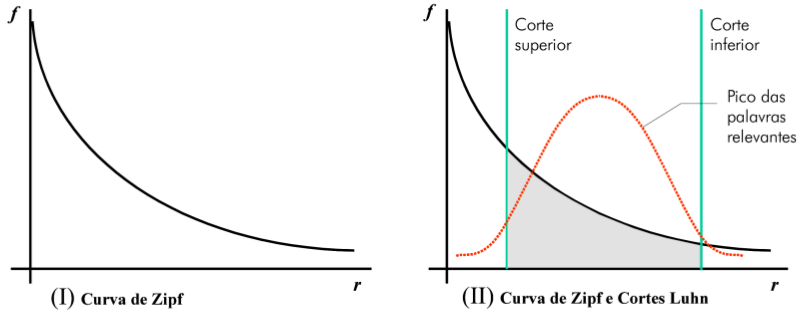
\includegraphics[width=0.85\textwidth]{conteudo/capitulos/figs/luhn2.png}
	  \caption{A curva de Zipf e os cortes de Luhn~\cite{Soares2008}.}
	  \label{fig:luhn}
  \end{figure}



As palavras não removidas na seleção de termos passam ainda por um processo conhecido como \textit{stemming}.
A radicalização ou \textit{stemming} é a redução das variações de uma palavra ao seu provável radical ou stem a fim de associar palavras semelhantes e diminuir a dimensionalidade da representação do texto.
Nesse processo, as palavras são reduzidas ao seu provável radical ou \textit{stem}, a fim de se associar palavras semelhantes e diminuir a dimensionalidade da representação do texto. Por exemplo, os termos ``\textit{agenda}'', ``\textit{agendamento}'' e ``\textit{agendar}'' dever ser todas reduzidas ao seu radical em comum ``\textit{agend}''. Com isso, a dimensionalidade é diminuída e tem-se um texto formado apenas por morfemas\footnote{Em Morfologia, um morfema é a menor unidade capaz de expressar significado.} com maior significância.  
% 
% O algoritmo de Porter, proposto por Martin Porter em 1980 é amplamente utilizado em sistemas que processam texto na língua inglesa e frequentemente eficaz na remoção de sufixos. Por outro lado, insuficiente para outros idiomas, uma vez que, seu mecanismo é altamente dependente do idioma inglês.
%

Em geral, algoritmos de \textit{stemming} dependem do uso adequado da ortografia da língua em questão, inclusive com acentuação correta, sendo em alguns casos recomendado o uso de corretores automáticos na fase de pré-processamento. A língua portuguesa particularmente apresenta algumas dificuldades, na elaboração de algoritmos de \textit{stemming}, das quais destacam-se o número elevado exceções e homófagos; palavras com mudanças no radical morfológico; nomes próprios que não podem ser radicalizados e frequência de termos estrangeiros.  É possível identificar alguns erros apresentados pelos algoritmos de \textit{stemming} que reduzem a qualidade os resultados da mineração de texto, como \textit{oversteamming:} quando o algoritmo remove parte do radical e \textit{understeamming:} quando o algoritmo não remove totalmente o sufixo.

O uso de \textit{stemming}, de uma maneira geral, pode trazer algumas desvantagens das como a perda de contexto, pois palavras com sentidos diferentes podem resultar no mesmo radical, aumentando assim a quantidade de homônimos e a perca da precisão que diminui a variedade de palavras causando certa perda de informação. Contudo, eventuais perdas de informação por \textit{stemming} não causam grandes impactos sobre a eficiência de algoritmos de text mining e seu uso se justifica pela redução da dimensionalidade da base de textos.





% -> Medidas utilizadas nessa dissertação
\documentclass{article} 
\begin{document} 
\begin{tabular}{|l|c|c|c|c|c|c|} 
\hline 
Configuração & \textbf{Pk} & \textbf{WD} & \textbf{A } & \textbf{P } & \textbf{R } & \textbf{F1}\\ \hline
TextTiling 20  3 & 0.288 & 0.494 & 0.506 & 0.503 & \textbf{0.886} & 0.618\\ \hline
TextTiling 20  6 & 0.228 & 0.472 & 0.528 & 0.515 & 0.725 & 0.579\\ \hline
TextTiling 20  9 & 0.192 & 0.459 & 0.541 & 0.533 & 0.643 & 0.549\\ \hline
TextTiling 20 12 & 0.163 & 0.456 & 0.544 & 0.555 & 0.489 & 0.495\\ \hline
TextTiling 30  3 & 0.265 & 0.481 & 0.519 & 0.510 & 0.863 & 0.615\\ \hline
TextTiling 30  6 & 0.201 & 0.445 & 0.555 & 0.538 & 0.766 & 0.605\\ \hline
TextTiling 30  9 & 0.171 & 0.434 & 0.566 & 0.563 & 0.667 & 0.580\\ \hline
TextTiling 30 12 & 0.168 & 0.445 & 0.555 & 0.582 & 0.457 & 0.485\\ \hline
TextTiling 40  3 & 0.252 & 0.491 & 0.509 & 0.509 & 0.815 & 0.599\\ \hline
TextTiling 40  6 & 0.212 & 0.452 & 0.548 & 0.537 & 0.735 & 0.593\\ \hline
TextTiling 40  9 & 0.154 & 0.401 & 0.599 & 0.612 & 0.572 & 0.563\\ \hline
TextTiling 40 12 & 0.202 & 0.498 & 0.502 & 0.503 & 0.363 & 0.394\\ \hline
TextTiling 50  3 & 0.224 & 0.454 & 0.546 & 0.534 & 0.809 & 0.617\\ \hline
TextTiling 50  6 & 0.137 & 0.387 & 0.613 & 0.631 & 0.661 & 0.612\\ \hline
TextTiling 50  9 & 0.143 & 0.446 & 0.554 & 0.584 & 0.458 & 0.483\\ \hline
TextTiling 50 12 & 0.181 & 0.468 & 0.532 & 0.557 & 0.388 & 0.427\\ \hline
TextTiling 60  3 & 0.218 & 0.476 & 0.524 & 0.525 & 0.728 & 0.580\\ \hline
TextTiling 60  6 & 0.173 & 0.494 & 0.506 & 0.516 & 0.474 & 0.468\\ \hline
TextTiling 60  9 & 0.162 & 0.450 & 0.550 & 0.582 & 0.437 & 0.471\\ \hline
TextTiling 60 12 & 0.158 & 0.469 & 0.531 & 0.549 & 0.379 & 0.419\\ \hline
C99 20  9 false & 0.158 & 0.482 & 0.518 & 0.579 & 0.182 & 0.267\\ \hline
C99 20  9 true & \textbf{0.135} & 0.457 & 0.543 & \textbf{0.654} & 0.225 & 0.323\\ \hline
C99 20 11 false & 0.158 & 0.476 & 0.524 & 0.600 & 0.188 & 0.277\\ \hline
C99 20 11 true & 0.146 & 0.458 & 0.542 & 0.649 & 0.216 & 0.313\\ \hline
C99 30  9 false & 0.177 & 0.490 & 0.510 & 0.525 & 0.276 & 0.346\\ \hline
C99 30  9 true & 0.153 & 0.443 & 0.557 & 0.613 & 0.346 & 0.422\\ \hline
C99 30 11 false & 0.167 & 0.486 & 0.514 & 0.534 & 0.285 & 0.355\\ \hline
C99 30 11 true & 0.164 & 0.454 & 0.546 & 0.595 & 0.326 & 0.403\\ \hline
C99 40  9 false & 0.163 & 0.459 & 0.541 & 0.564 & 0.436 & 0.469\\ \hline
C99 40  9 true & 0.151 & 0.398 & 0.602 & 0.645 & 0.502 & 0.540\\ \hline
C99 40 11 false & 0.163 & 0.465 & 0.535 & 0.555 & 0.431 & 0.462\\ \hline
C99 40 11 true & 0.169 & 0.419 & 0.581 & 0.617 & 0.465 & 0.507\\ \hline
C99 50  9 false & 0.172 & 0.456 & 0.544 & 0.542 & 0.560 & 0.530\\ \hline
C99 50  9 true & 0.154 & \textbf{0.383} & \textbf{0.617} & 0.619 & 0.645 & 0.610\\ \hline
C99 50 11 false & 0.169 & 0.451 & 0.549 & 0.548 & 0.569 & 0.538\\ \hline
C99 50 11 true & 0.158 & 0.401 & 0.599 & 0.600 & 0.626 & 0.591\\ \hline
C99 60  9 false & 0.178 & 0.450 & 0.550 & 0.540 & 0.671 & 0.577\\ \hline
C99 60  9 true & 0.182 & 0.411 & 0.589 & 0.573 & 0.704 & 0.609\\ \hline
C99 60 11 false & 0.178 & 0.456 & 0.544 & 0.535 & 0.665 & 0.572\\ \hline
C99 60 11 true & 0.178 & 0.411 & 0.589 & 0.573 & 0.709 & 0.611\\ \hline
C99 70  9 false & 0.213 & 0.472 & 0.528 & 0.518 & 0.746 & 0.589\\ \hline
C99 70  9 true & 0.209 & 0.440 & 0.560 & 0.541 & 0.782 & 0.617\\ \hline
C99 70 11 false & 0.193 & 0.448 & 0.552 & 0.535 & 0.782 & 0.612\\ \hline
C99 70 11 true & 0.212 & 0.439 & 0.561 & 0.542 & 0.781 & 0.617\\ \hline
C99 80  9 false & 0.247 & 0.485 & 0.515 & 0.508 & 0.826 & 0.606\\ \hline
C99 80  9 true & 0.227 & 0.443 & 0.557 & 0.535 & 0.870 & \textbf{0.638}\\ \hline
C99 80 11 false & 0.242 & 0.470 & 0.530 & 0.517 & 0.845 & 0.618\\ \hline
C99 80 11 true & 0.227 & 0.443 & 0.557 & 0.535 & 0.870 & \textbf{0.638}\\ \hline
\end{tabular} 
\end{document} 
 

% -> Recuperação de Informação
\section{Recuperação de Informação}

% Necessidade de encontrar informação

Devido à popularização dos computadores e à grande disponibilidade de documentos em formato digital, em especial na Web a área da Recuperação de Informação (RI) tem recebido atenção de pesquisadores nas últimas décadas.
% 
Recuperação de informação é área da computação que envolve a aplicação de métodos computacionais no tratamento e busca de informação em bases de dados não estruturados, usualmente grandes coleções de documentos textuais armazenados em dispositivos eletrônicos.
% Tratamento == Classificação e Agrupamento?
A tarefa central da recuperação de informação é encontrar informações de interesse dos usuários e exibi-las. A principal ferramenta empregada nesse problema é o desenvolvimento de sistemas de recuperação de informação (SRI). Nesses sistemas o usuário expressa sua necessidade por meio da formulação de uma consulta, usualmente composta por um conjunto de palavras-chave. Então, o sistema apresenta os resultados da busca, frequentemente documentos, em ordem de relevância com a consulta.



\subsection{Modelos de Recuperação de Informação}

Um modelo de recuperação de informação deve criar representações de documentos e consultas a fim de predizer a necessidade expressa nos termos da consulta. Com base na entrada do usuário esses modelos buscam por documentos similares aos termos da consulta. Segue abaixo a descrição dos três modelos clássicos para recuperação de informação.

\subsubsection{Modelo Booleano}

O modelo booleano ou modelo lógico foi um dos primeiros modelos aplicados a recuperação informação sendo utilizado a partir de 1960. Nesse modelo uma consulta é considerada uma sequencia de termos conectador por operadores lógicos como AND, OR e NOT. Como resultado, classifica cada documento como relevante ou não relevante à consulta, sem gradação de relevância. Esse operadores lógicos poder ser manipulados por usuários com algum conhecimento em álgebra booleana para aumentar a quantidade de resultados ou restringi-la.

Esse modelo apresenta como principal desvantagem a impossibilidade de ordenação dos resultados por relevância, uma vez que para muitos sistemas de RI o \textit{ranking} dos resultados é uma característica essencial, principalmente em grades bases de dados. 

As vantagens desse modelo são a facilidade de implementação e a possibilidade de usuários experientes usarem os operadores lógicos como uma forma de controle sobre os resultados da busca. Por outro lado, para usuários inexperientes isso pode ser considerado uma desvantagem, uma vez que o uso expressões lógicas não é intuitivo. Apesar dos problemas apresentados, visto sua simplicidade, esse modelo foi largamente utilizado em sistemas comerciais. 



\subsubsection{Modelo Vetorial}


Uma das formas mais comuns para representação textual é conhecida como Modelo Espaço Vetorial (\textit{Vectorial Space Model} - VSM)~\cite{Rezende2003}, onde os documentos e consultas são representados como vetores em um espaço Euclidiano $t$-dimensional em que cada termo extraído da coleção é representado por uma dimensão. 
% 
Considera-se que um documento pode ser representado pelo seu conjunto de termos, onde cada termo $k_i$ de um documento $d_j$ associa-se um peso $w_{ij}\geq0$ que indica a importância desse termo no documento. 
%
De forma similar, para uma consulta $q$, associa-se um peso $w_{i,q}$ ao par termo consulta que representa a similaridade entre a necessidade do usuário e o termo $k_i$. 
%
Assim o vetor associado ao documento $d_j$ é dado por $\vec{d}_{j} = (w_{1,j}, w_{2,j}, ..., w_{t,j})$. 
%
De forma similar, o vetor associado a consulta $q$ é dado por $\vec{q} = (w_{1,q}, w_{2,q}, ..., w_{t,q})$.


No modelo vetorial, a similidade entre um documento $d_j$ e uma consulta $q$ é calculada pela correlação entre os vetores $\vec{d_j}$ e $\vec{q}$, a qual pode ser medida pelo cosseno do  ângulo entre esses vetores, conforme mostrado na Equação~\ref{equ:cosseno-doc-consulta}.



\begin{equation}
sim(d_j, q) = \frac{ \vec{d_j} \bullet \vec{q} }
                   { |\vec{d_j}| \times | \vec{q}|}
            = \frac{ \sum_{i=1}^{t} w_{i,j} \cdot w_{i,q} }
                   { \sqrt{\sum_{i=1}^{t} w_{i,j}^2} \times \sqrt{\sum_{i=1}^{t} w_{i,q}^2 } }                   \label{equ:cosseno-doc-consulta}		                   
\end{equation} 


Valores de cosseno próximos a 0 indicam um ângulo próximo a 90º entre $\vec{d_j}$ e $\vec{q}$, ou seja, o documento $d_j$ compartilha poucos termos com a consulta $q$, enquanto valores próximos a 1 indicam um ângulo próximo a 0º, ou seja, $d_j$ e $q$ compartilham termos e são similares~\cite{Tan2005,Feldman2006}.

Avaliar a relevância de um documento sob uma consulta é fundamental para os modelos de RI. Para isso pode-se utilizar medidas estatísticas simples como a frequência do termo, conhecida como TF (do inglês \textit{Term Frequency}) e a frequência de documentos, conhecida como DF (do inglês \textit{Document Frequency}). A frequência do termo indica o número de vezes que um termo ocorre na coleção de documentos. A frequência de documentos, indica o número de documentos que contém ao menos uma ocorrência de um determinado termo. Considera-se que os termos que ocorrem frequentemente em muitos documentos, em geral, não trazem informações úteis para discriminar a relevância dos documentos, então, a fim de diminuir o peso de termos altamente frequentes, usa-se o fator IDF (\textit{Inverted Document Frequency}), que é o inverso da número de documentos que contem um termo. O IDF é a medida de informação que um termo fornece com base em quão raro ou comum esse termo é para a coleção. Seja $N$ o número de documentos de uma coleção e $n_i$ o número de documentos onde o termo $k_i$ ocorre, o cálculo de IDF é dado por: 

	\begin{equation}
		IDF(k_i) = log\frac{N}{n_i}
		\label{equ:IDF}
	\end{equation}

Entre a medidas mais populares para ranqueamento de buscas está a TF-IDF (\textit{Term Frequency-Inverted Document Frequency}) que pondera a frequência de um termo em um documento com sua frequência na coleção total de documentos. Assim, a relevância de um termo para um documento é dada por:

\begin{equation}
	w_{i,j} = freq_{i,j} \cdot IDF(k_i)
\end{equation}



Onde $freq_{i,j}$ é a frequência do termo $k_i$ no documento $d_j$. A medida TF-IDF atribui valores altos para termos que ocorrem frequentemente em um documentos, e valores menores para termos que ocorrem poucas vezes em um documento ou em muitos documentos da coleção. A ideia da medida tf.idf e quantificar a importância de um termo em um documento com base em sua frequência no próprio documento e sua distribuição ao longo da coleção de documentos~\cite{Croft2009,Salton1988,Shamsinejadbabki2012,Salton:1994}.


Uma vez que o sistema calcula os graus de similaridade entre os documentos e a busca por meio da equação~\ref{equ:cosseno-doc-consulta}, é possível ranquear os resultados por ordem de relevância. Além disso, sua relativa simplicidade e flexibilidade, favorecem a aplicação desse modelo em sistemas de recuperação de informação
~\cite{Tan2005,Croft2009,Manning2008}.

% ->-----------------------------------------------------------------------


\subsubsection{Modelo Probabilístico}

 
O modelo probabilístico é baseado no princípio da ordenação probabilística (\textit{Probability Ranking Principle}) onde dada um consulta q e um documento $d_j$ relevante a $q$, o modelo tenta estimar a probabilidade do usuário encontrar o documento $d_j$. O modelo assumente que para uma consulta $q$ há um conjunto de documentos $R$ que contém exatamente os documentos relevantes e nenhum outro, sendo este um conjunto resposta ideal que maximiza a probabilidade do usuário encontrar um documento $d_j$ relevante a $q$. 

Seja $\overline{R_q}$ o complemento de $R$ de forma que $\overline{R_q}$ contém todos os documentos não relevantes à consulta $q$. Seja $P(R_q|d_j)$ a probabilidade do documento $d_j$ ser relevante à consulta $q$ e $P(\overline{R_q}|d_j)$ a probabilidade de $d_j$ não ser relevante à $q$. A similaridade entre um documento $d_j$ e uma consulta $q$ é definida por:


\begin{equation}
	sim(d_j, q) = \frac{P(R_q|dj)}{P(\overline{R_q}|dj)}
\end{equation}


% -> Explicar o (odds ratio)


% -> Segmentação 

\documentclass{sig-alternate-05-2015}
\usepackage[portuguese]{babel}
%\usepackage{multirow}
%\usepackage{adjustbox}
%\usepackage{graphicx}
%\usepackage{array}
%\usepackage{tabulary}
% \usepackage{pgfplotstable}
% recommended:
%\usepackage{booktabs}
%\usepackage{array}
%\usepackage{colortbl}
%\usepackage{emptypage}
%\newcolumntype{l}[1]{>{\centering\arraybackslash}p{#1}}
% \usepackage{showframe}   %% just for demo
% \usepackage[brazilian,hyperpageref]{backref}	 % Paginas com as citações na bibl
% \usepackage[alf]{abntex2cite}	% Citações padrão ABNT
\usepackage[utf8]{inputenc}		% Codificacao do documento (conversão automática dos acentos)

\usepackage{rotating}
\usepackage{tabularx}
\usepackage{multicol}
\usepackage{amsmath}
\usepackage[linesnumbered,ruled]{algorithm2e}




% Define o caminho das figuras
\graphicspath{{images/}}



\begin{document}

\title{Segmentação topical automática de atas de reunião}


\numberofauthors{1} 

\author{
\alignauthor Ovídio José Francisco\\
       \email{ovidiojf@gmail.com}
}

\maketitle

%\begin{abstract}   
%
%\end{abstract}

\section*{RESUMO}



\keywords{}

\begingroup
\let\clearpage\relax

\section{Introdução}
	\label{sec:introducao}
	Frequentemente atas de reunião tem a característica de apresentar um texto com poucas quebras de parágrafo e sem marcações de estrutura, como capítulos, seções ou quaisquer indicações sobre o tema do texto. 


% Definição 

A tarefa de segmentação textual consiste dividir um texto em partes que contenham um significado relativamente independente. Em outras palavras, é identificar as posições onde há uma mudança significativa de tópicos.

% Usos
É útil em aplicações que trabalham com textos sem quebras de assunto, ou seja, não apresentam parágrafos, seções ou capítulos, como transcrições automáticas de áudio e grandes documentos que contêm assuntos não idênticos como atas de reunião e noticias.


% Interesses
O interesse por segmentação textual tem crescido em em aplicações voltadas a recuperação de informação %citar o [15] ...
e sumarização de textos. % ... e [2] do "Efficient Linear T S"
Essa técnica pode ser usada para aprimorar o acessao a informação quando essa é solicitada por um usário por meio de uma consulta, onde é possível oferecer porções menores de texto mais relevante ao invés de exibir um documento maior que pode conter informações menos pertinente. A sumarização de texto também pode ser aprimorada ao processar segmentos separados por tópicos ao invés de documentos inteiros.


% Coesão Léxica
Os algoritmos avaliados baseiam-se na ideia de coesão léxica entre assuntos. Isto é, a mudança de tópicos é acompanhada % é relacionada à
 de uma proporcional mudança de vocabulário. A partir disso, vários algorítmos foram propostos. Nesse artigo, os principais serão analizados na prespectiva de atas de reunião.





% Diversas aplicações fazem uso de segmentação textual, incluindo 

% Entre as principais mais frequentes de segmentação textual estão a tra



%É principalmente utilizada em aplicações que processam textos longos como transcrições de áudio e documentos longos, além de aprimorar técnicas de sumarização e information retrievel.



% Usos:
%	* quando não há identificações
%	* em transcrições de áudio
%	* em documentos longos
% 	* text summarization (ver a referencia [2] de Efficient Linear Text...)




%Isto é, dado um texto, identificar onde há mudança de tópicos.


% Interest in automatic text segmentation has blossomed over the last few years, with applications ranging from information retrieval to text summariza-tion to story segmentation of video feeds. [A Critique and Improvement of an Evaluation Metric for Text Segmentation]



%Em outras palavras é identificar divisões entre unidade de informação sucessivas

%A tarefa de segmentação textual consiste em encontrar pontos onde há mudança de tópicos no texto.



%[ The task of linear text segmentation is to split a large text document into shorter fragments, usually blocks of consecutive sentences. ]


% **Segmentação é identificar divisiões entre unidades de informação sucessivas (Beeferman, Berger, and Lafferty (1997))**

%   [Text segmentation is the task of determining the positions at which topics change in a stream of text]






\section{Trabalhos Relacionados}
	\label{sec:trabalhos}
	\section{Trabalhos Relacionados}
	\label{sec:trabalhos}


Semelhante a esse trabalho, outras abordagens foram propostas como em~\cite{CHAIBI2014} onde os autores adaptam os \textit{TextTiling} e \textit{C99} ao idioma árabe. Apresentam os resultados de experimentos no qual avaliam a performance em jornais de diferentes países em árabe. As adaptações consistem basicamente na etapa de pré-processamento e apontam que diferenças no dialeto de cada pais devem ser consideradas no processo de segmentação e que a adaptação depende da escolha de um \textit{stemmer} adequado.

É recorrente a aplicação de segmentadores à reuniões com múltiplos participantes onde se estuda os discursos extraídos de reuniões, ou seja, o texto a ser segmentado é uma transcrição das falas dos participantes durante a reunião.
%
Banerjee~\cite{Banerjee2006} apresenta um segmentador baseado no  \textit{TextTiling} ao contexto das reuniões, com múltiplos participantes. Utiliza como \textit{corpus} a transcrição da fala dos participantes durante a reunião a qual foi conduzida por um mediador que propunha os tópicos e anotava o tempo onde os participantes mudavam o assunto. 
% outros exemplos são

Ainda no contexto de reuniões com múltiplos participantes, alguns elementos da fala são utilizados para encontrar melhores segmentos.
%
Bokaei~\cite{Bokaei2015}, traz um trabalho voltado à segmentação funcional do texto, que foca na atividade dos participantes, as quais categoriza em diálogos e monólogos e sugere que alguns comportamentos podem dar pistas de mudança de tópico, como quando um participante toma a palavra por um tempo prolongado. 
Galley~\cite{Galley2003} por sua vez considera de elementos como pausas, trocas de falantes e entonação para encontrar melhores segmentos.

Kern aponta em sua pesquisa~\cite{Kern2009} que algoritmos que apresentam melhor performance o fazem ao custo de maior complexidade computacional, que se deve à construção de matrizes de similaridade entre todas as sentenças como em~\cite{Choi2000}. Ele apresenta uma abordagem que otimiza o cálculo ao computar as médias das similaridades de cada bloco, a qual chama de \textit{inner similarity} e em seguida usa esses valores para calcular as medias das similaridades entre todos os blocos a qual chama de \textit{outter similarity}. Dessa forma não é criada uma matriz que contem as similaridades de todas as sentenças, mas apenas daquelas mais próximas. Os autores reportam uma eficiência superior e uma eficiência comparável aos algoritmos mais complexos.
% usa vetores contendo o peso da palavra ao inves da frequencia.




\section{Adaptação às atas de reunião}
	\label{sec:adaptacaoasatas}
	\section{Proposta: Segmentação Linear Automática de Atas de Reunião}
	\label{sec:proposta}






%%%%%%%%%%
% TextTiling e C99 criados para inglês e independente de domínio
%%%%%%%%%%
Os algoritmos \textit{TextTiling} e \textit{C99} foram propostos para o inglês, independentemente de domínio, ou seja, a proposta inicial dos autores é trabalhar em qualquer texto nessa língua.
%%%%%%%%%%
% Adapatar para Atas em português
%%%%%%%%%%
Assim, propõe-se adaptá-los ao contexto das atas de reunião em português do Brasil, ou seja, em uma língua diferente e dentro de um contexto específico. As subseções seguintes tratam das adaptações para esse nicho mais específico. A Seção~\ref{sec:avaliacao} mostra a análise dos algoritmos adaptados.

%%%%%%%%%%
% Dificuldade: Coesão léxica não tão bem definida
%%%%%%%%%%
O vocabulário das reuniões, ainda que em tópicos diferentes, compartilham certo vocabulário pertencente ao ambiente onde se deram as reuniões. Isso é um fator que diminui a coesão léxica entre os segmentos.
%%%%%%%%%%
% Dificuldade: estilo da escrita
% - Paragrafo único
% - Cabeçalhos e rodapés
% - Pontuação --> ; encerrando sentenças
% - Insersão de espaços que não são quebra de sentença
% - Ruídos
%%%%%%%%%%
As atas de reunião costumam ter um estilo de escrita que deve ser levado em conta na adaptação do algoritmos, como a identificação de finais de sentença na ausência de quebras de parágrafo, inserção de linhas que não separam assuntos, utilização de pontuação para transição de tópicos, e cabeçalhos e numerais ruidosos. 

Nas subseções a seguir serão apresentados o pré-processamento e a identificação de segmentos candidatos considerados para a segmentação de atas.





\subsection{Pré-processamento}
	\label{subsec:preprocessamento}




	O texto a ser segmentado frequentemente é extraído de documentos em formatos como \textit{pdf}, \textit{doc}, \textit{docx} ou \textit{odt}. Após a extração do texto, esse pode passar por processos de transformação os quais serão apresentados a seguir.
	
%	A etapa de pré-processamento, em um documento contendo texto puro, acontece em quatro passos principais. 

  \begin{figure}[!h]
	\centering
	
\includegraphics[width=0.2\textwidth]{construcao.png}
%	\caption{Exemplo de pré-processamento.}
	\\Em Construção
	\label{fig:exemplopreprocessamento}
  \end{figure}

	
%\begin{enumerate}


%
% 1) Identificação de sentenças
%\item \textit{Identificação de sentenças}: 
%Cada final de sentença e identificado e marcado com uma \textit{string} especial, esse processo é melhor descrito na Subseção~\ref{subsec:indentificacaosentencas}.
%
%conforme mostrado no Algoritmo~\ref{alg:identificacaofinaisdesent}.

%	
% 2) Eliminação de ruídos
%\item \textit{Remoção de ruídos}:

%%%%%%%%%%
% Cabeçalhos e rodapés
%%%%%%%%%%
%As atas frequentemente contém trechos que podem ser considerados pouco informativos e descartados durante o pré-processamento, como cabeçalhos e rodapés que se misturam aos tópicos tratados na reunião, podendo ser  inseridos no meio de um tópico e criando uma quebra que prejudica tanto o algoritmo de segmentação, quanto a leitura do texto pelo usuário.
%%%%%%%%%%
% Numerais
%%%%%%%%%%
%Também é comum o uso de numerais para marcação de páginas e linhas, da mesma forma, são pouco informativos e podem ser descartados.


%%%%%%%%%%
% Remoção de ruídos
%%%%%%%%%%
%Nesse trabalho, esses elementos são removidos, uma vez que, o descarte não causa perca de informação e pode facilitar a identificação dos segmentos, pois melhora a coesão do texto. Outro benefício é manter o texto livre de trechos que fogem do assunto circundante.
%%%
% TODO: Como são removidos?
% por meio de heurísticas simples
%%%

%Elimina-se também nesse passo a acentuação, sinais de pontuação, restando apenas palavras.  



%	
% 3) Stop Words
%\item \textit{Stop Words}: 
%Remove-se as palavras consideradas menos informativas, as quais são chamadas de \textit{stop words}, para isso, utiliza-se uma lista contendo 438 palavras. 

%
% 4) Stemming
%\item \textit{Stemming}:
%Extrai-se o radical de cada palavra, para isso, as letras são convertidas em caixa baixa e aplica-se o algoritmo \textit{Orengo}\footnote{\urlorengo} para remoção de sufixos.


%\end{enumerate}
	
	



%Tem-se então, uma lista com os elementos considerados mais significativos do texto. %A Figura~\ref{fig:exemplopreprocessamento} mostra a etapa de pré-processamento em uma sentença em português.
	



%  \begin{figure}[!h]
%	\centering
%	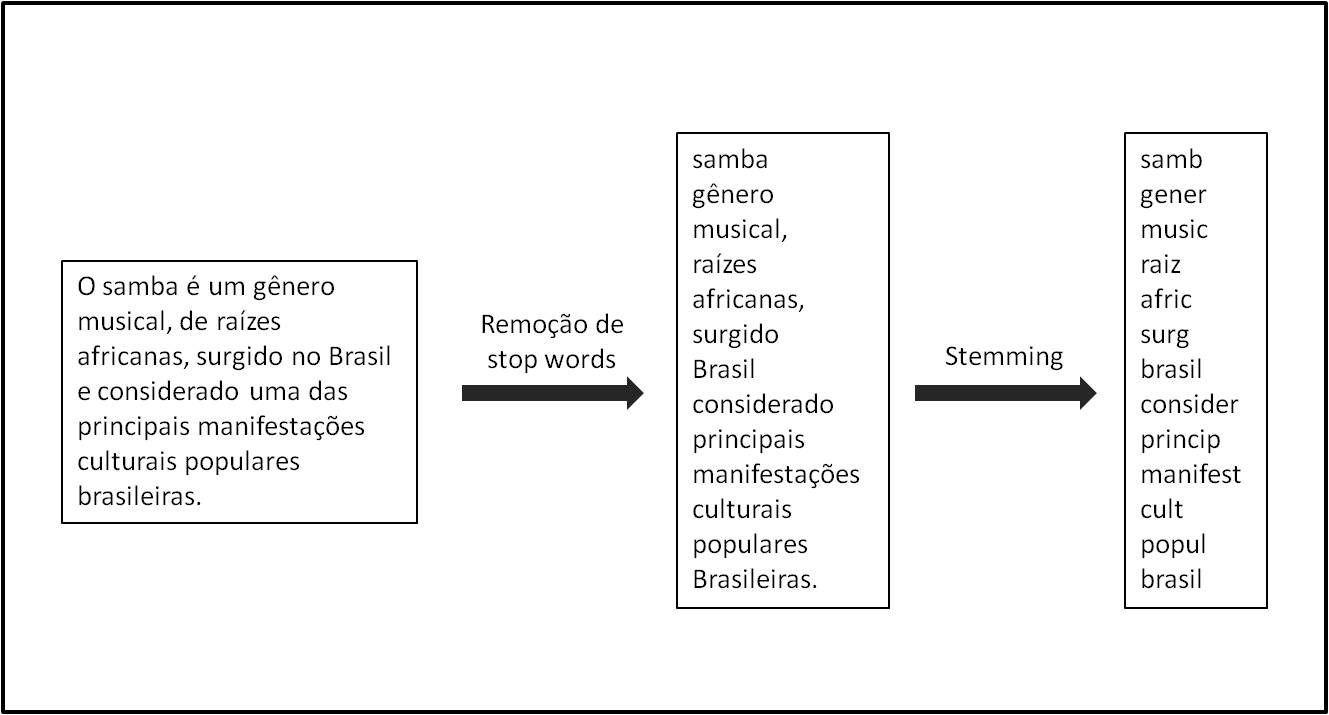
\includegraphics[width=0.45\textwidth]{exemplo-preprocessamento.jpg}
%	\caption{Exemplo de pré-processamento.}
%	\label{fig:exemplopreprocessamento}
%  \end{figure}






\subsection{Identificação de candidatos}
	\label{subsec:indentificacaosentencas}
	
%%%%%%%%%%	
% Indicar unidade mínima de Segmento
%%%%%%%%%%
	
	
%	Como entrada para os 
%	Os algoritmos de segmentação devem ser
	É preciso fornecer aos algoritmos os candidatos iniciais a limites de segmento. Para isso, é necessário escolher qual será a unidade de informação mínima que constitui um segmento. Baseando-se no estilo de escrita e considerando as pontuações de um texto, é possível, em alguns casos, indicar quebras de parágrafo, finais de sentenças ou mesmo palavras como elementos que encerram um segmento. 

	Ocorre que em atas de reunião é uma prática comum redigi-las de forma que o conteúdo discutido fica em parágrafo único, além disso, as quebras de parágrafo são usados para formatação de outros elementos como espaço para assinaturas. 
%
	Também não é conveniente indicar todo ponto entre \textit{token} como candidato pois obrigaria a ajustar posteriormente os segmentos de maneira a não quebrar uma ideia ou frase. 
%	
	Assim, neste trabalho, os finais de sentença são considerados unidades de informação e portanto, passíveis a limite entre segmentos. 
	
	Devido ao estilo de pontuação desses documentos, como encerrar sentenças usando um \textit{";"} e inserção de linhas extras, foram usadas as regras apresentadas no Algoritmo 1 para identificar os finais de sentenças.  


\begin{algorithm}
	\SetKwInOut{Input}{Entrada}
	\SetKwInOut{Output}{Saída}
	\SetKwBlock{Inicio}{início}{fim}
	\SetKwFor{ParaTodo}{para todo}{}{fim para todo}
	\SetKwIF{Se}{SenaoSe}{Senao}{}{}{senao se}{senao}{fim se}
	\SetKwFor{Para}{}{}{}
%	\SetKwAlgorithm{Algorithm}{Algoritmo}{}

	
	\Input{Texto}
	\Output{Texto com identificações de finais de sentença}
	
	\ParaTodo {token, marcá-lo como final de sentença se:} {	

	Terminar com um \texttt{!}\\
	Terminar com um \texttt{.} e não for uma abreviação\\
	Terminar em \texttt{.?;} e:
		\Para{}{
			For seguido de uma quebra de parágrafo ou tabulação\\
			O próximo \textit{token} iniciar com  \texttt{(\{["'}\\
			O próximo \textit{token} iniciar com letra maiúscula\\
			O penúltimo caracter  for \texttt{)\}]"'}\\
		}
	}
	
	\caption{Identificação de finais de sentença}
	\label{alg:identificacaofinaisdesent}
\end{algorithm}









%Como forma de padronização, as instituições acrescentam ao documento

%		passos menores
%		1 - heurística simples para remover cabeçalho e rodapé.
%		2 - remoção de numerais
%		3 - remoção de acentos, transformações de caixa, remoção de pontuação.
		
	% Esses passos são realizados internamente em cada algorímo, para que a saida seja legível ao usuário final.





%A qualidade do algoritmo é sempre dependente da escrita correta! Ausência de emoticons, códigos de computador e gírias.





%Nas subseções a seguir serão expostas as alterações para aumentar a eficiência dos algoritmos e encontrar o melhor modelo para a tarefa de segmentar o texto das atas em tópicos.



%Tais aspectos não se aplicam ao contexto das atas, onde o estilo de escrita em forma de narrativa, prefere poupar o leitor de diálogos secundários durante transições de tópicos. 







	
	
%Elimina-se textos considerados de pouca relevância como a numeração de páginas e linhas, cabeçalhos e rodapés, também elemina-se acentuação, sinais de pontuação, restando apenas palavras.  


	
	
%%
%% 1) Identificação de sentenças
%Primeiro cada final de sentença e identificado e marcado com uma \textit{string} especial, esse processo é melhor descrito na Subseção~\ref{subsec:indentificacaosentencas}.
%%
%%conforme mostrado no Algoritmo~\ref{alg:identificacaofinaisdesent}.
%
%%	
%% 2) Eliminação de ruídos
%Depois, elimina-se textos considerados de pouca relevância como a numeração de páginas e linhas, cabeçalhos e rodapés, também elemina-se acentuação, sinais de pontuação, restando apenas palavras.  
%
%%	
%% 3) Stop Words
%Em seguida, remove-se as palavras consideradas menos informativas, as quais são chamadas de \textit{stop words}, para isso, utiliza-se uma lista contendo 438 palavras. 
%
%%
%% 4) Stemming
%Por fim, extrai-se o radical de cada palavra, para isso, as letras são convertidas em caixa baixa e aplica-se o algoritmo \textit{Orengo}\footnote{\urlorengo} para remoção de sufixos.
%
%
%Tem-se então, uma lista com os elementos considerados mais significativos do texto. A Figura~\ref{fig:exemplopreprocessamento} mostra a etapa de pré-processamento em uma sentença em português.
%	





	

\section{Avaliação}
	\label{sec:avaliacao}
	
\section{Avaliação}
	\label{sec:avaliacao}



%%%%%%%%%% 
% Necessidade de uma referência
%%%%%%%%%%
Para que se possa avaliar um segmentador automático de textos, é preciso uma referência, isto é, um texto com os limites entre os segmento conhecidos. Essa referência, deve ser confiável, sendo uma segmentação legítima que é capaz de dividir o texto em porções relativamente independentes, mantendo um conteúdo legível, ou seja, uma segmentação ideal.
%

Entre as abordagens mais comuns para se conseguir essas referências, encontramos: A concatenação aleatória de documentos distintos, onde o ponto entre o final de um texto e o inicio do seguinte é um limite entre eles. A segmentação manual dos documentos, nesse caso, pessoas capacitadas, também chamadas de juízes, ou mesmo o autor do texto, são consultadas e indicam manualmente onde há uma quebra de segmento. Em transcrição de conversas faladas em reuniões com múltiplos participantes, um mediador é responsável por encerrar um assunto e iniciar um novo, nesse caso o mediador anota manualmente o tempo onde há uma transição de tópico. Em aplicações onde a segmentação é tarefa secundária, analisar seu impacto na aplicação final.


%%%%%%%%%%
% As 2 principais dificuldades na avaliação
%%%%%%%%%%
De acordo com \cite{Pevzner2002} há duas principais dificuldades na avaliação de segmentadores automáticos. A primeira é conseguir um referência, já que juízes humanos costumam não concordar entre si, sobre onde os limites estão e outras abordagens podem não se aplicar ao contexto. A segunda é que tipos diferentes de erros devem ter pesos diferentes de acordo com a aplicação. Há casos onde certa imprecisão é tolerável e outras, como a segmentação de notícias, onde a precisão é mais importante.


%%%%%%%%%%
% Definição do que é um bom algoritmo de segmentação
%%%%%%%%%%
Para fins de avaliação desse trabalho, um bom método de segmentação é aquele cujo resultado melhor se aproxima do ideal, sem a obrigatoriedade de estar perfeitamente alinhado com tal. Ou seja, visto o contexto das atas de reunião, e a subjetividade da tarefa, não é necessário que os limites entre os segmentos (real e hipótese) sejam idênticos, mas que se assemelhem em localização e quantidade.


Para quantificar a eficiência dos algoritmos, segue uma revisão das principais métricas aplicáveis.

As próximas subseções mostram o conjunto de atas e a segmentação usada como referência, uma revisão das principais métricas aplicáveis à segmentação e os testes realizados a fim de avaliar os métodos

\subsection{Conjunto de documentos}
	A fim de obter um conjunto de documentos segmentados que possam servir como referência na avaliação, seis atas de reunião foram coletadas junto ao departamento de computação da UFSCar-Sorocaba. Os documentos foram oferecidos à profissionais que participam de reuniões desse departamento e por meio de um \textit{software} segmentaram o texto das atas conforme o julgamento de cada um. Os segmentos gerados manualmente foram comparados à segmentação automática conforme os critérios descritos a seguir.
	
	As atas de reunião diferem dos textos comumente estudados em outros trabalho em alguns pontos.
	


\subsection{Medidas de Avaliação}


	As medidas de avaliação tradicionalmente utilizadas em \textit{information retrieval} como precisão e revocação trazem alguns problemas na avalização de segmentadores automáticos.  
Conforme o algoritmo aponta mais segmentos no texto, tende a melhorar a revocação e ao mesmo tempo, reduzir a precisão, um problema que pode ser contornado usando \textit{F-measure} que faz uma combinação da duas levando em conta seus pesos, o que por outro lado é mais difícil de interpretar. 
Essas medidas falham ao não serem sensíveis a \textit{near misses}, ou seja, quando um limite não coincide exatamente com o esperado, mas fica próximo~\cite{Kern2009}.

A Figura~\ref{fig:exemplosegmentacaozoom} mostra um exemplo com duas segmentações hipotéticas e uma referência. Em ambos os casos não há nenhum verdadeiro positivo, o que implica em zero para os valores de precisão, acurácia, e revocação, embora a segunda hipótese possa ser considerada superior à primeira se levado em conta a proximidade dos limites.



  \begin{figure}[!h]

	\centering
	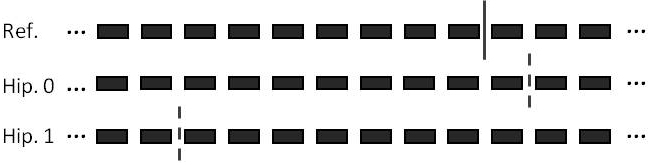
\includegraphics[width=0.47\textwidth]{windiffzoom.jpg}
	\caption{Exmplos de segmentação}
	\label{fig:exemplosegmentacaozoom}

  \end{figure}



\subsubsection{P$_k$}
A fim de resolver o problema de \textit{near misses}, Beeferman \textit{et. al.}~\cite{Beeferman1999} apresentam uma nova medida chama P$_k$ que atribui valores parciais a \textit{near misses}. Esse método move uma janela de tamanho $k$ e a cada posição e verifica se o início e o final da janela estão ou não dentro do mesmo segmento e penaliza o algoritmo em caso de discrepância. 

Ou seja, dado duas palavras de distancia $k$, uma discrepância é computada quando o algoritmo e a referência não concordam se as palavras estão ou não no mesmo segmento.

O valor de $k$ é calculado como a metade da média dos comprimentos dos segmentos reais. Como resultado, é retornado a contagem de discrepâncias divido pelo quantidade de segmentações analisadas. Esse valor serve como medida de dissimilaridade entre as segmentações e pode ser interpretada como a probabilidade de duas sentenças extraídas aleatoriamente pertencerem ao mesmo segmento.



\subsubsection{WindowDiff}

Pevzner~\cite{Pevzner2002} aponta problemas na avaliação mais tradicional Pk~\cite{Beeferman1999}. Eles apontam que esse método penaliza demasiadamente os falsos negativos em relação aos falsos positivos e a \textit{near misses}, além disso, desconsidera o tamanho e a quantidade de segmentos, entre outros problemas.

Como solução, propõem um novo método, o qual chamam de \textit{WindowDiff} que traz duas diferenças principais: a dobra a penalidade para os falsos positivos a fim de diminuir o problema da subestimação dessa medida e, diferente de P$_k$, ao mover a janela pelo texto, penaliza o algoritmo sempre que o número de limites proposto pelo algoritmo não coincidir com o número de limites esperados para aquela janela de texto. 

Com isso, demonstram em seu trabalho que, em relação a P$_k$, consegue resolver seus principais problemas e mantém sua proposta inicial de sensibilidade a \textit{near misses}, penalizando-os menos que os falsos positivos puros.


  \begin{figure}[!h]

	\centering
	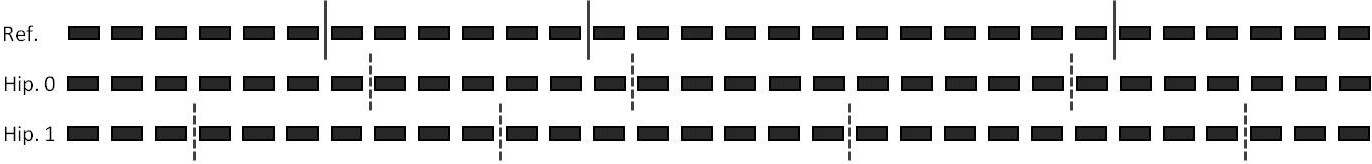
\includegraphics[width=0.47\textwidth]{windiff.jpg}
	\caption{Exemplo de construção de uma matriz de rank}
	\label{fig:exemplosegmentacao}

  \end{figure}
  
  

%Falar do software para segmentação manual????


\subsection{Avaliação dos segmentadores}


%%%%%%%%%%
% Parâmetros
%%%%%%%%%%
As implementações dos algoritmos permitem ao usuário a configuração de seus parâmetros. 
%
O \textit{TextTiling} permite ajustarmos dois parâmetros, sendo, o tamanho da janela (distância entre a primeira e a última sentença) para o qual atribuiu-se os valores 20, 40 e 60. O segundo parâmetro, o passo (distância que a janela desliza), atribuiu-se os valores 3, 6, 9 e 12. Gerando ao final 18 modelos.
%

O \textit{C99} permite ajustarmos três parâmetros, sendo, a quantidade segmentos desejados, o qual é calculado como uma proporção dos candidatos a limite. Para isso atribuiu-se as proporções de 0,2 a 1,0 em intervalos de 0,2 O segundo parâmetro, o tamanho da máscara utilizada para gerar a matriz de ranking, atribuiu-se os valores 9 e 11. Permite ainda, definirmos se as sentenças serão representados por vetores contendo a frequência ou o peso de cada termo, onde ambas as representações foram utilizadas. Gerando ao final 20 modelos.



%%%%%%%%%%
% Cálculo das medidas para cada modelo
%%%%%%%%%%
Pela comparação dos resultados com a segmentação fornecida pelos especialistas, calculou-se para cada modelo as medidas tradicionais acurácia, precisão, revocação, F-medida. Além dessas, computou-se também as métricas mais aplicadas à segmentação textual P$_k$ e \textit{WindowDiff}.



%%%%%%%%%%
% Teste de Fiedman e CD
% 1ª Etapa
%%%%%%%%%%
Em seguida aplicou-se o teste de Friedman a fim de saber se há diferenças significativas entre a eficácia dos modelos, o pós-teste de Nemenyi foi aplicado para descobrir quais diferenças são significativas. 
%
Exite diferença quando seus \textit{rankings} médios diferirem em um valor mínimo, chamado de diferença critica (CD). 
%

%%%%%%%%%%
% Dados Obtidos
%%%%%%%%%%
Com isso foi possível, pela análise do diagrama de diferença crítica, verificar qual é o melhor modelo para cada medida
% e quão significativamente 
em relação aos demais. 


A tabela~\ref{tab:mediasC99} mostra os dados obtidos com o \textit{C99}, onde \texttt{S} é a proporção de segmentos em relação a quantidade de candidatos, \texttt{M} é o tamanho da máscara utilizada para criar a matriz de \textit{ranking} e \texttt{W} indica se os segmentos são representados por vetores contendo a frequência ou um peso das palavras. 



\begin{table}[!h]
	\centering

	\begin{tabular}{|c|c|c|c|c|}
	
		\hline
		Medida & \texttt{S} & \texttt{M} & \texttt{W} & \textbf{Média}\\		
		\hline

		Acuracy		& 40	& 11 & Sim & 0.6199	\\ \hline	
		F1			& 60	& 9	 & Sim & 0.6167	\\ \hline	
		Precision	& 40	& 11 & Sim & 0.7106	\\ \hline			
		Recall		& 100	& 9	 & Não & 0.8516	\\ \hline		
		Pk			& 40	& 11 & Sim & 0.1163	\\ \hline	
		Windiff		& 40	& 11 & Sim & 0.3800	\\ \hline		

		
	\end{tabular}
	
	\caption{Médias das medidas obtidas com \textit{C99}}
	\label{tab:mediasC99}
\end{table}


A tabelas~\ref{tab:mediasTextTiling} mostra os dados obtidos com o \textit{TextTiling}, \texttt{J} é o tamanho da janela e \texttt{P} e o passo.

\begin{table}[!h]
	\centering

	\begin{tabular}{|c|c|c|c|}
	
		\hline
		Medida & \texttt{J} & \texttt{P} & \textbf{Média}\\		
		\hline

		Acuracy		& 50 & 9 	& 0.5510 \\ \hline	
		F1			& 50 & 3 	& 0.5898 \\ \hline	
		Precision	& 60 & 12 	& 0.5746 \\ \hline			
		Recall		& 50 & 3 	& 0.7717 \\ \hline		
		Pk			& 30 & 9 	& 0.1572 \\ \hline	
		Windiff		& 50 & 9 	& 0.4489 \\ \hline		

		
	\end{tabular}
	
	\caption{Médias das medidas obtidas com o \textit{TextTiling}}
	\label{tab:mediasTextTiling}
\end{table}


Uma vez sabendo quais valores de parâmetros melhor configuram um algoritmo para uma medida, resta então saber qual dos dois algoritmos é mais eficiente segundo essa medida. Para isso aplicou-se novamente o teste de Friedman com pós-teste de Nemenyi, dessa vez, com os melhores modelos dos dois algoritmos para cada medida. O resultado segue na Tabela~\ref{tab:melhoresmodelos}

\begin{table}[!h]
	\centering
	
	\begin{tabular}{|c|c|c|c|c|}

		\hline
		Medida & Algoritmo & \texttt{S} & \texttt{M} & \texttt{W}\\		
		\hline
		
	
		Acuracy		& C99 & 40 	& 11	& Sim \\ \hline
		Precision	& C99 & 40 	& 11	& Sim \\ \hline
		Pk			& C99 & 40 	& 11	& Sim \\ \hline
		Windiff		& C99 & 40 	& 11	& Sim \\ \hline
		F1			& C99 & 60 	& 9		& Sim \\ \hline
		Recall		& C99 & 100 & 9		& Não \\ \hline
 	
	
	\end{tabular}

	\caption{Melhores modelos para cada medida segundo diagramas de diferença crítica}
	\label{tab:melhoresmodelos}	
	
\end{table}


Na análise do diagrama de diferença crítica verificou-se que o algoritmo \textit{C99} apresenta melhor eficiência em todas as medidas e os valores das quatro primeiras os valores de \texttt{S}, \texttt{M} e \texttt{W} se repetiram, sugerindo uma configuração otimizada para o problema da segmentação de atas de reunião.







	
\section{Análise dos Resultados}
	\label{sec:resultados}
	\section{Resultados}
	\label{sec:resultados}

%%%%%%%%%%
% Objetivos
%%%%%%%%%%
A fim de encontrar o melhor método que divida uma ata em segmentos coerentes, realizou-se experimentos com o \textit{TextTiling} e \textit{C99} a fim de encontrar os melhores parâmetros para esses documentos.

%tópicos retornando segmentos  que retorne segmentos coerentes 

%%%%%%%%%%
% Parâmetros
%%%%%%%%%%
As implementações dos algoritmos permitem ao usuário a configuração de seus parâmetros. 
%
O \textit{TextTiling} permite ajustarmos dois parâmetros, sendo, o tamanho da janela (distância entre a primeira e a última sentença) para o qual atribuiu-se os valores 20, 40 e 60. Para o segundo parâmetro, o passo (distância que a janela desliza), atribuiu-se os valores 3, 6, 9 e 12. Gerando ao final 20 modelos.
%

O \textit{C99} permite ajustarmos três parâmetros, sendo, a quantidade segmentos desejados, o qual é calculado como uma proporção dos candidatos a limite. Para isso atribuiu-se as proporções {0,2; 0,4; 0,6; 0,8; 1,0}. O segundo parâmetro, o tamanho da máscara utilizada para gerar a matriz de ranking, atribuiu-se os valores 9 e 11. Permite ainda, definirmos se as sentenças serão representados por vetores contendo a frequência ou o peso de cada termo, onde ambas as representações foram utilizadas.
%
 Considerando todos os parâmetros, foram gerados 20 modelos para o algoritmo C99.% By Rafael 



%%%%%%%%%%
% Cálculo das medidas para cada modelo
%%%%%%%%%%

% --> Isso já foi falado no texto
%Pela comparação dos resultados com a segmentação fornecida pelos especialistas, calculou-se para cada modelo as medidas tradicionais acurácia, precisão, revocação, F-medida. Além dessas, computou-se também as métricas mais aplicadas à segmentação textual P$_k$ e \textit{WindowDiff}.



%%%%%%%%%%
% Teste de Fiedman e CD
% 1ª Etapa
%%%%%%%%%%
Em seguida aplicou-se o teste de Friedman a fim de saber se há diferenças significativas entre a eficácia dos modelos. O pós-teste de Nemenyi foi aplicado para descobrir quais diferenças são significativas. 
%
Exite diferença quando seus \textit{rankings} médios diferirem em um valor mínimo, chamado de diferença critica (CD). 
%

%%%%%%%%%%
% Dados Obtidos
%%%%%%%%%%
Com isso foi possível, pela análise do diagrama de diferença crítica, verificar qual é o melhor modelo para cada medida
% e quão significativamente 
em relação aos demais. 


A Tabela~\ref{tab:mediasC99} mostra os dados obtidos com o \textit{C99}, onde \texttt{S} é a proporção de segmentos em relação a quantidade de candidatos, \texttt{M} é o tamanho da máscara utilizada para criar a matriz de \textit{ranking} e \texttt{W} indica se os segmentos são representados por vetores contendo a frequência ou um peso das palavras. 



\begin{table}[!h]
	\centering

	\begin{tabular}{|c|c|c|c|c|}
	
		\hline
		Medida & \texttt{S} & \texttt{M} & \texttt{W} & \textbf{Média}\\		
		\hline

		Acuracy		& 40	& 11 & Sim & 0.6199	\\ \hline	
		F1			& 60	& 9	 & Sim & 0.6167	\\ \hline	
		Precision	& 40	& 11 & Sim & 0.7106	\\ \hline			
		Recall		& 100	& 9	 & Não & 0.8516	\\ \hline		
		Pk			& 40	& 11 & Sim & 0.1163	\\ \hline	
		Windiff		& 40	& 11 & Sim & 0.3800	\\ \hline		

		
	\end{tabular}
	
	\caption{Médias das medidas obtidas com \textit{C99}}
	\label{tab:mediasC99}
\end{table}


A tabelas~\ref{tab:mediasTextTiling} mostra os dados obtidos com o \textit{TextTiling}, onde \texttt{J} é o tamanho da janela e \texttt{P} é o passo.

\begin{table}[!h]
	\centering

	\begin{tabular}{|c|c|c|c|}
	
		\hline
		Medida & \texttt{J} & \texttt{P} & \textbf{Média}\\		
		\hline

		Acuracy		& 50 & 9 	& 0.5510 \\ \hline	
		F1			& 50 & 3 	& 0.5898 \\ \hline	
		Precision	& 60 & 12 	& 0.5746 \\ \hline			
		Recall		& 50 & 3 	& 0.7717 \\ \hline		
		Pk			& 30 & 9 	& 0.1572 \\ \hline	
		Windiff		& 50 & 9 	& 0.4489 \\ \hline		

		
	\end{tabular}
	
	\caption{Médias das medidas obtidas com o \textit{TextTiling}.}
	\label{tab:mediasTextTiling}
\end{table}


Uma vez sabendo quais valores de parâmetros melhor configuram um algoritmo para uma medida, resta então saber qual dos dois algoritmos é mais eficiente segundo essa medida. Para isso aplicou-se novamente o teste de Friedman com pós-teste de Nemenyi, dessa vez, com os melhores modelos dos dois algoritmos para cada medida. O resultado segue na Tabela~\ref{tab:melhoresmodelos}

\begin{table}[!h]
	\centering
	
	\begin{tabular}{|c|c|c|c|c|}

		\hline
		Medida & Algoritmo & \texttt{S} & \texttt{M} & \texttt{W}\\		
		\hline
		
	
		Acuracy		& C99 & 40 	& 11	& Sim \\ \hline
		Precision	& C99 & 40 	& 11	& Sim \\ \hline
		Pk			& C99 & 40 	& 11	& Sim \\ \hline
		Windiff		& C99 & 40 	& 11	& Sim \\ \hline
		F1			& C99 & 60 	& 9		& Sim \\ \hline
		Recall		& C99 & 100 & 9		& Não \\ \hline
 	
	
	\end{tabular}

	\caption{Melhores modelos para cada medida segundo diagramas de diferença crítica.}
	\label{tab:melhoresmodelos}	
	
\end{table}


Na análise do diagrama de diferença crítica verificou-se que o algoritmo \textit{C99} apresenta melhor eficiência em todas as medidas e os valores das quatro primeiras os valores de \texttt{S}, \texttt{M} e \texttt{W} se repetiram, sugerindo uma configuração otimizada para o problema da segmentação de atas de reunião.






	
\section{Conclusão}
	\label{sec:conclusao}
	\section{Conclus�o}
	\label{sec:conclusao}

As atas de reuni�o, objeto de estudo desse artigo, apresentam caracter�sticas peculiares em rela��o � discursos e textos em geral. Caracter�sticas como segmentos curtos e coes�o mais fraca devida ao estilo que evita repeti��o de palavras e ideias em benef�cio da leitura por humanos, dificultam o processamento por computadores.

%%%%%%%%%%
% Benef�cios 
%%%%%%%%%%


Os algoritmos \textit{TextTiling} e \textit{C99} foram testados em um conjunto de atas coletadas do Departamento de Computa��o da UFSCar-Sorocaba. Por meio da an�lise dos dados chegou-se a uma configura��o cujos segmentos melhor se aproximaram das amostras segmentadas por participantes das reuni�es. 


Na maioria das medidas, o algoritmo \textit{C99} sobressaiu-se em rela��o ao \textit{TextTiling}, contudo, os testes estat�sticos, n�o apresentam diferen�a significativa. 


%%%%%%%%%%%%%%%
% O Impacto do Preprocessamento 
%%%%%%%%%%%%%%%

Da mesma forma, a etapa de preprocessamento proporciona melhora de performance quando aplicada, por�m o seu maior benef�cio � a diminui��o do custo computacional, uma vez que n�o prejudica a qualidade dos resultados.



A segmenta��o de atas de reuni�o pode ajudar na organiza��o, busca e compreens�o dos conte�dos nelas contidos. Tamb�m outros dom�nios e aplica��es diferentes podem se beneficiar dos resultados apresentados, como aplica��es voltadas a resgate de informa��o, sumariza��o e acessibilidade. Assim, espera-se que outros trabalhos possam aproveitar deste.
	
	
Em trabalhos futuros, ser�o investigadas t�cnicas de extra��o de t�picos para descrever os segmentos e com isso aprimorar o acesso ao conte�do das atas de reuni�o.





\endgroup



\bibliographystyle{abbrv}
\bibliography{sigproc}  % sigproc.bib is the name of the Bibliography in this case
	
\pagestyle{empty}
 	\label{sec:anexo}
 	\include{project/anexo}
\end{document}


% -> Anotações
\section{Anotação de Subtópicos}

A avaliação de segmentadores frequentemente requer uma segmentação de referência. Essa referência deve refletir um segmentação real sendo confiável para apoiar a avaliação da qualidade de técnicas de segmentação. 

A construção de um corpus anotado demanda tempo e disponibilidade de anotadores humanos, o que a torna uma tarefa relativamente custosa. 
Assim, é necessário seguir procedimentos que assegurem que a tarefa seja concluída com o exito esperado que o resultado produzido seja válido, confiável e consistente para fins de pesquisas científicas. Para isso,~\cite{Hovy2010} propuseram uma metodologia para anotação em corpus que pode ser resumida em sete passos: 
(1) Escolha do evento a ser anotado, %e a teoria que o embasa,
(2) Seleção do corpus,% apropriado,
(3) Selecionar e treinar os anotadores,
(4) Especificar o processo de anotação,
(5) Modelar uma interface para anotação,
(6) Escolher e aplicar medidas de avaliação e 
(7) Disponibilizar e manter o produto.
% 
A seguir, serão descritos outros trabalhos relacionados a anotação de corpus e em seguida a os passos dessa metodologia. %  propostos por~\cite{Hovy2010}.

Um dos primeiros trabalhos a produzir um corpus com anotações de segmentos foi~\cite{Hearst1997} no qual um corpus constituído por doze artigos de revistas foram anotados por sete técnicos pesquisadores. Cada artigo continha entre 1.800 e 2500 palavras. O autor considerou um limite entre segmentos real onde pelo menos três anotadores marcavam uma transição de tópico. No trabalho de~\cite{Kazantseva2012} utilizou-se um livro ficcional contendo vinte capítulos que foi segmentado por seis alunos de graduação que além de marcar os pontos de transição entre segmentos, forneceram um descrição breve sobre cada segmento identificado. 

Outros trabalhos abordaram corpus compostos pela transcrição de audios. Por exemplo,~\cite{Passonneau1997} transcreveu vinte narrativas sobre um filme que foi segmentada e anotada por sete voluntários. Cada narrativa, continha cerca de 13.500 palavras. Os anotadores não receberam nenhum treinamento formal para a tarefa, mas apenas foram solicitados a usar suas noções de comunicabilidade para identificar as mudanças de tópicos. No trabalho de~\cite{Galley2003} investigou-se a transcrição de um conjunto de vinte e cinco reuniões obtidas do \textit{ICSI Meeting corpus}~\cite{Janin2003} em que pelo menos três anotadores analisaram os pontos onde ocorreu troca da pessoa que fala e apontaram como sendo ou não uma mudança de assunto.  

Nesses trabalhos utilizou-se os anotadores como juízes para produzir uma referência em que decidiu-se sobre cada candidato a limite entre segmentos por meio da opinião da maioria. Além desses trabalhos, outros se valeram de segmentações produzidas artificialmente. Por exemplo,~\cite{Choi2000} produziu um corpos formado por 700 documentos. As referências foram geradas pela concatenação de sentenças extraídas de documentos diferentes. De maneira semelhante,~\cite{CHAIBI2014} utilizou a concatenação de artigos de noticias para produzir os documentos. Os autores consideram um limite real o ponto que divide dois artigos originais. 

\subsection{Metodologia para anotações em corpus}
\label{subsec:anotacoes}


Os trabalhos citados anteriormente utilizaram procedimentos diferentes para produzir segmentações de referência para seus trabalhos. Como já citado,~\cite{Hovy2010} propôs que o processo de anotação em corpus pode der sintetizado e dividido em sete passos. 


\subsubsection{Escolha do corpus}
A criação de corpus raramente é restrita a um único propósito. O material original deve ser preferencialmente constituído de documentos disponíveis livremente à comunidade, a fim de facilitar a comparação, extensão e avaliação de trabalhos futuros. 
Devido a diversidade linguística de diferentes domínios e gêneros de textos, a escolha dos documentos de amostra deve procurar ser representativa ao domínio a ser abordado. O corpus é considerado representativo quando o assunto a abordado na amostra tem correspondência com a interpretação do público geral desse domínio.

% \subsubsection{Fundamentação da teoria}
\subsubsection{Escolha da teoria a ser explicada}
A anotação deve ajudar a explicar uma teoria, ou seja, fornecer informações úteis à sua compreensão. Essa teoria irá guiar a especificação do processo de anotação, quais informações deseja-se extrair e como interpretá-las. Quanto mais complexa for a teoria ser explicada, mais complexa será a tarefa de anotação bem como as instruções que os anotadores deverão seguir. Além disso, deve-se estabelecer de início o nível de detalhamento necessário. 
A complexidade da teoria e nível de detalhamento impactam na condução da anotação e da estabilidade da anotação.

% quanto é necessário se aprofundar em detalhes


\subsubsection{Selecionar e treinar os anotadores}

O treinamento e o nível de conhecimento dos anotadores ainda é uma questão em aberto. Alguns pesquisadores afirmam que estes devem ser especialistas no domínio do corpus. Outros afirmam que pessoas adequadamente treinadas podem produzir resultados satisfatórios. 
Considerando a necessidade de treinamento, tem-se a subjetividade das tarefas que dificulta a elaboração de instruções precisas. Tarefas que permitem a especificação de procedimentos que levam em conta a possibilidade de diferentes casos e variáveis, põem em dúvida a necessidade da criação de um corpus anotado.
Por outro lado, a ausência de treinamento implica que as anotações terão como base o conhecimento prévio dos anotadores e sua preconcepção a cerca do domínio o que diminui o nível de concordância entre os anotadores e dificulta a replicação de outros trabalhos.


\subsubsection{Especificar o procedimento de anotação}
Alguns processos de anotações podem levar longos períodos, criando a necessidade de dividir a tarefa em fases. Nesses casos, frequentemente os anotadores fazem reuniões periódicas a fim de relatar eventuais problemas.  
% Em alguns projetos, abre-se espaço para discussão de pontos com baixa concordância, a qual é chamada de fase de ``reconciliação''. 
Em caso de baixa concordância, pode-se abrir espaço para discussão de pontos com baixa concordância, a qual é chamada de fase de ``reconciliação'' que embora recomendada, em alguns casos pode ocasionar um enviesamento dos resultados. Outra estratégia para baixa concordância é que solicitar que os anotadores marquem o nível de certeza sobre as anotações.
% Essa fase é recomendada para aumentar o nível de concordância, contudo pode ocasionar um enviesamento dos resultados. 

\subsubsection{Modelar uma interface para anotação}
Um software com interface amigável, além de facilitar o trabalho, evita erros durante o processo. 
O ganho em tempo e a melhoria na qualidade dos resultados justifica a criação de uma interface. 
Exemplos softwares para anotação na área de Processamento de linguagem natural e Bioinformática podem ser encontrados em~\cite{Gruenstein2007}.



\subsubsection{Escolher e aplicar medidas de avaliação}

Quando observa-se baixa concordância entre os anotadores, entende-se que há uma falha no processo de anotação ou na teoria a ser explicada, o que implica que o dados produzidos não servem para a fins de pesquisa ou aplicações práticas. A medida dessa concordância deve determinar a confiabilidade dos resultados.
A medida mais utilizada em Processamento de linguagem natural é o coeficiente \textit{kappa}~\cite{Carletta1996} que retorna um valor no intervalo de 0 até 1, onde 1 significa uma concordância perfeita e 0 que não houve concordância. Seja, $P(A)$ a proporção de vezes que os anotadores concordam e $P(E)$ a proporção de concordância esperada ao acaso. O cálculo de \textit{kappa} é dado por:

\begin{equation}
	kappa = \frac{P(A) - P(E)}{1 - P(E)}
\end{equation}

Essa medida, apresenta como limitação a entrada de apenas dois casos. Como alternativa, a medida conhecida como \textit{Fleiss's k}~\cite{Fleiss1979} pode ser utilizada quando há mais que dois anotadores, porém restringe-se a anotações com apenas duas categorias. 
Na avaliação de segmentadores, as medidas $P_k$ (Equação~\ref{equ:Pk}) e \textit{WindowDiff} (Equação~\ref{equ:windiff}) podem ser utilizadas, uma vez que são medidas de similaridade, como visto em~\cite{Kazantseva2012,Cardoso2017}.



\subsubsection{Disponibilizar e manter o produto}

Uma vez criado, o corpus anotado deve ser disponibilizado para uso em outros trabalhos. 
Recomenda-se fornecer o corpus original além dos resultados obtidos, observando-se desde o início e ao longo do tempo a propriedade e eventuais licenças sob o corpus original.






% -> Extração de Tópicos
\section{Modelos de Extração de Tópicos}

% Na venda do peixe, citar que a busca é tão difícil quanto a leitura e análise de coleções de documentos.

Os modelos de extração de tópicos são abordagens não-supervisionadas que visam descobrir padrões latentes nas relações entre os documentos e seus termos.  Baseiam-se na premissa de que um documento é produzido a partir de tópicos previamente definidos que determinam os termos a serem utilizados em um documento. Nesse contexto, um documento é uma mistura de tópicos onde cada termo presente no documento pode ser associado a um tópico. Um tópico por sua vez, é uma estrutura com valor semântico que representada por um conjunto de termos e seus pesos que indicam o quão significante esses termos são para um assunto e pode ser útil para o entendimento do tema ao qual o tópico trata.

Para descobrir esses tópicos, algumas técnicas foram propostas. Em termos de metodologia, a maioria dos trabalho enquadram-se em duas principais categorias, os modelos não-probabilísticos e os modelos probabilísticos.


% -- \subsection{Modelos Não Probabilísticos}

Os modelos não-probabilísticas baseiam-se em técnicas de fatoração de matrizes, onde a matrix documento-termo é projetada em um espaço com menor dimensionalidade chamado \textit{Latent Semantic Space}. 
Seja
$d \in D = \{d_1,\cdots,d_n\}$ o vetor que representa a coleção de documentos, 
$t \in T = \{t_1,\cdots,t_m\}$ seus termos distintos e 
$z \in Z = \{z_1,\cdots,z_k\}$ seus tópicos. 
Esses métodos aprendem decompondo a matriz documento-termo $W$, em duas matrizes $Z$ e $A$, tal que a resultante de $ZA$ seja uma aproximação da matriz $W$ original. Mais formalmente tem-se:

\begin{equation}
	Z\cdot A = \hat{W} \approx W
\end{equation}

A matriz $A$ corresponde a matriz documento-tópico e possui dimensão $k \times n$. $Z$ corresponde a matriz termo-tópico e possui dimensão $m \times k$ onde $n$ é o número de termos, $m$ é o número de documentos da coleção e $k$ é a quantidade de tópicos a serem extraídos. Uma vez que $k \ll n,m$, então $A$ e $Z$ são menores que a matriz de entrada, o que resulta em uma versão comprimida da matriz original, pois $k \cdot n + m \cdot k \ll n \cdot m$. Ao final, obtém-se uma representação documento-tópico que atribui um peso para cada tópico em cada documento da coleção e uma representação termo-tópico que representa a probabilidade de ocorrência de um termo em um documento dado que o tópico está presente no documento.

 Nesse sentido, o \textit{Latente Semantic Indexing} (LSI) usa a técnica chamada \textit{Singular Value Decomposition} (SVD) para encontrar padrões no relacionamento entre assuntos e termos em uma coleção de texto não estruturada. Entretanto, esse método não fornece uma interpretação para elementos com valores negativos~\cite{Deerwester1990}~\cite{Cheng2013}. % Trocar essa referência do Cheng2013 pela que ele usa na seção 2 do trabalho dele.

% -- NMF
Outro modelo popular é o \textit{Non-Negative Matrix Factorization} (NMF).  Diferente do LSI, no processo de fatoração apenas operações aditivas são permitidas, o que garante que as matrizes resultantes não possuem elementos negativos, permitindo uma interpretação mais intuitiva de seus valores. Além disso, o processo de fatoração proporciona a propriedade de \textit{clustering}, ou seja, agrupar as colunas da matriz $W$, e dessa forma, oferece a característica interessante de agrupar os documentos da coleção.  % -< Onde é utilizado


% -- \subsection{Modelos Probabilísticos}

Os modelos probabilísticos consideram os documentos como uma mistura de tópicos e um tópico como uma distribuição probabilística sobre os termos. O processo de elaboração do documento a partir desses tópicos é chamado de processo generativo ou modelo generativo, o qual é desconhecido porém pode ser estimado com base nos termos presentes no documento, também chamados de variáveis observáveis. Assim, o processo de extração de tópicos consiste em estimar o modelo generativo que deu origem ao documento.
% falar em algum ponto sobre o problema das matrizes esparsas. Principalmente com documentos pequenos
% 
% -- PLSA
O PLSA foi um dos primeiros a estender o modelo LSA e formalizar a extração de tópicos probabilísticos. De maneira similar ao LSA, o esse modelo decompõe uma matriz esparsa a fim de reduzir a dimensionalidade. O PLSA cria um modelo estatístico chamado \textit{aspect model} que associa os tópicos as variáveis observáveis atribuindo probabilidades às ligações entre os tópicos e os documentos e entre as palavras e os tópicos. Assim, cada documento pode ser representado como a probabilidade de um tópico estar presente, $P(z|d)$. E a probabilidade de um termo ocorrer dado que um tópico esta presente, $P(t|z)$. Em comparação ao LSA, é considerado uma método mais robusto por proporcionar uma interpretação probabilística. Por outro lado, esse modelo apresenta desvantagens como o número de parâmetros do modelo que cresce linearmente com o número de documentos da coleção que pode ocasionar \textit{overfitting}.   % - E o Expectation Maximization?

% -- LDA
A fim de contornar esses problemas, o LDA estende o modelo PLSA incorporando um modelo generativo onde os cada tópico obedece à distribuição multivariada de \textit{Dirichlet} o que o torna menos propenso ao \textit{overfitting} e capaz de inferir tópicos a documentos ainda não observados. É referenciado na literatura como estado da arte sobre modelos probabilísticos de extração de tópicos e influencia uma grande quantidade de trabalhos, tornando-se base para novos modelos. No modelo LDA, o processo de geração de palavras se dá em duas etapas:

\begin{enumerate}
	\item Atribui-se uma distribuição aleatória sobre os tópicos.
	\item Para cada termo no documento:
		\begin{enumerate}
			\item Atribui-se aleatoriamente a um tópico da distribuição obtida na etapa 1;
			\item Seleciona-se aleatoriamente uma palavra do tópico correspondente.
		\end{enumerate}
\end{enumerate}

Assim cada documento é associado a múltiplos tópicos com proporções distintas (etapa 1). Cada palavra do documento é obtida de um tópico específico (etapa 2.b) que foi anteriormente obtido a partir da distribuição de tópicos do documento (etapa 2.a). Isso permite ao modelo LDA atribuir, para cada documento, múltiplos tópicos com proporções distintas~\cite{Blei2012}.

Os modelos de extração de tópicos foram inicialmente propostos para utilização em mineração texto onde são empregados na redução de dimensionalidade, extração de informações em textos, bem como na organização e recuperação de documentos, sendo utilizados para mensurar a relevância de um termo ou conjunto de termos para determinado assunto ou documento. Visto a popularidade nessas tarefas e flexibilidade dos modelos, logo notou-se sua utilidade em outros tipos de dados com atributos discretos como imagens, grafos e genética. 







\chapter{Sistema Proposto}\label{cap3}


Essa seção apresenta as etapas de desenvolvimento do sistema de recuperação de atas proposto, bem como o seu funcionamento geral, desde a preparação dos documentos até a entrega dos históricos de ocorrência ao usuário. Inicialmente serão descritos a seleção e pré-processamento das atas. Em seguida, será relatado como as técnicas de mineração de texto e recuperação de informação são utilizadas nesse trabalho.

A Figura \ref{fig:visao-geral} mostra a visão geral do sistema proposto cujo objetivo é permitir ao usuário consultar uma coleção de documentos de reuniões a fim de obter todo o histórico de ocorrências de um determinado tema relacionado à pesquisa do usuário, podendo identificar nos documentos onde esse tema foi mencionado, bem como se houve uma decisão sobre o tema. Para isso, o sistema é divido em dois módulos principais: módulo de preparação e manutenção e módulo de consulta, os quais serão detalhados nas próximas seções.  % "isso envolve a classificação. Onde entram os tópicos?" --> Rafael

A Figura \ref{fig:visao-geral} mostra a visão geral do sistema com suas principais entradas e saídas. 


  %--- Figura Visão Geral ---
  \begin{figure}[!h]
	  \centering
	  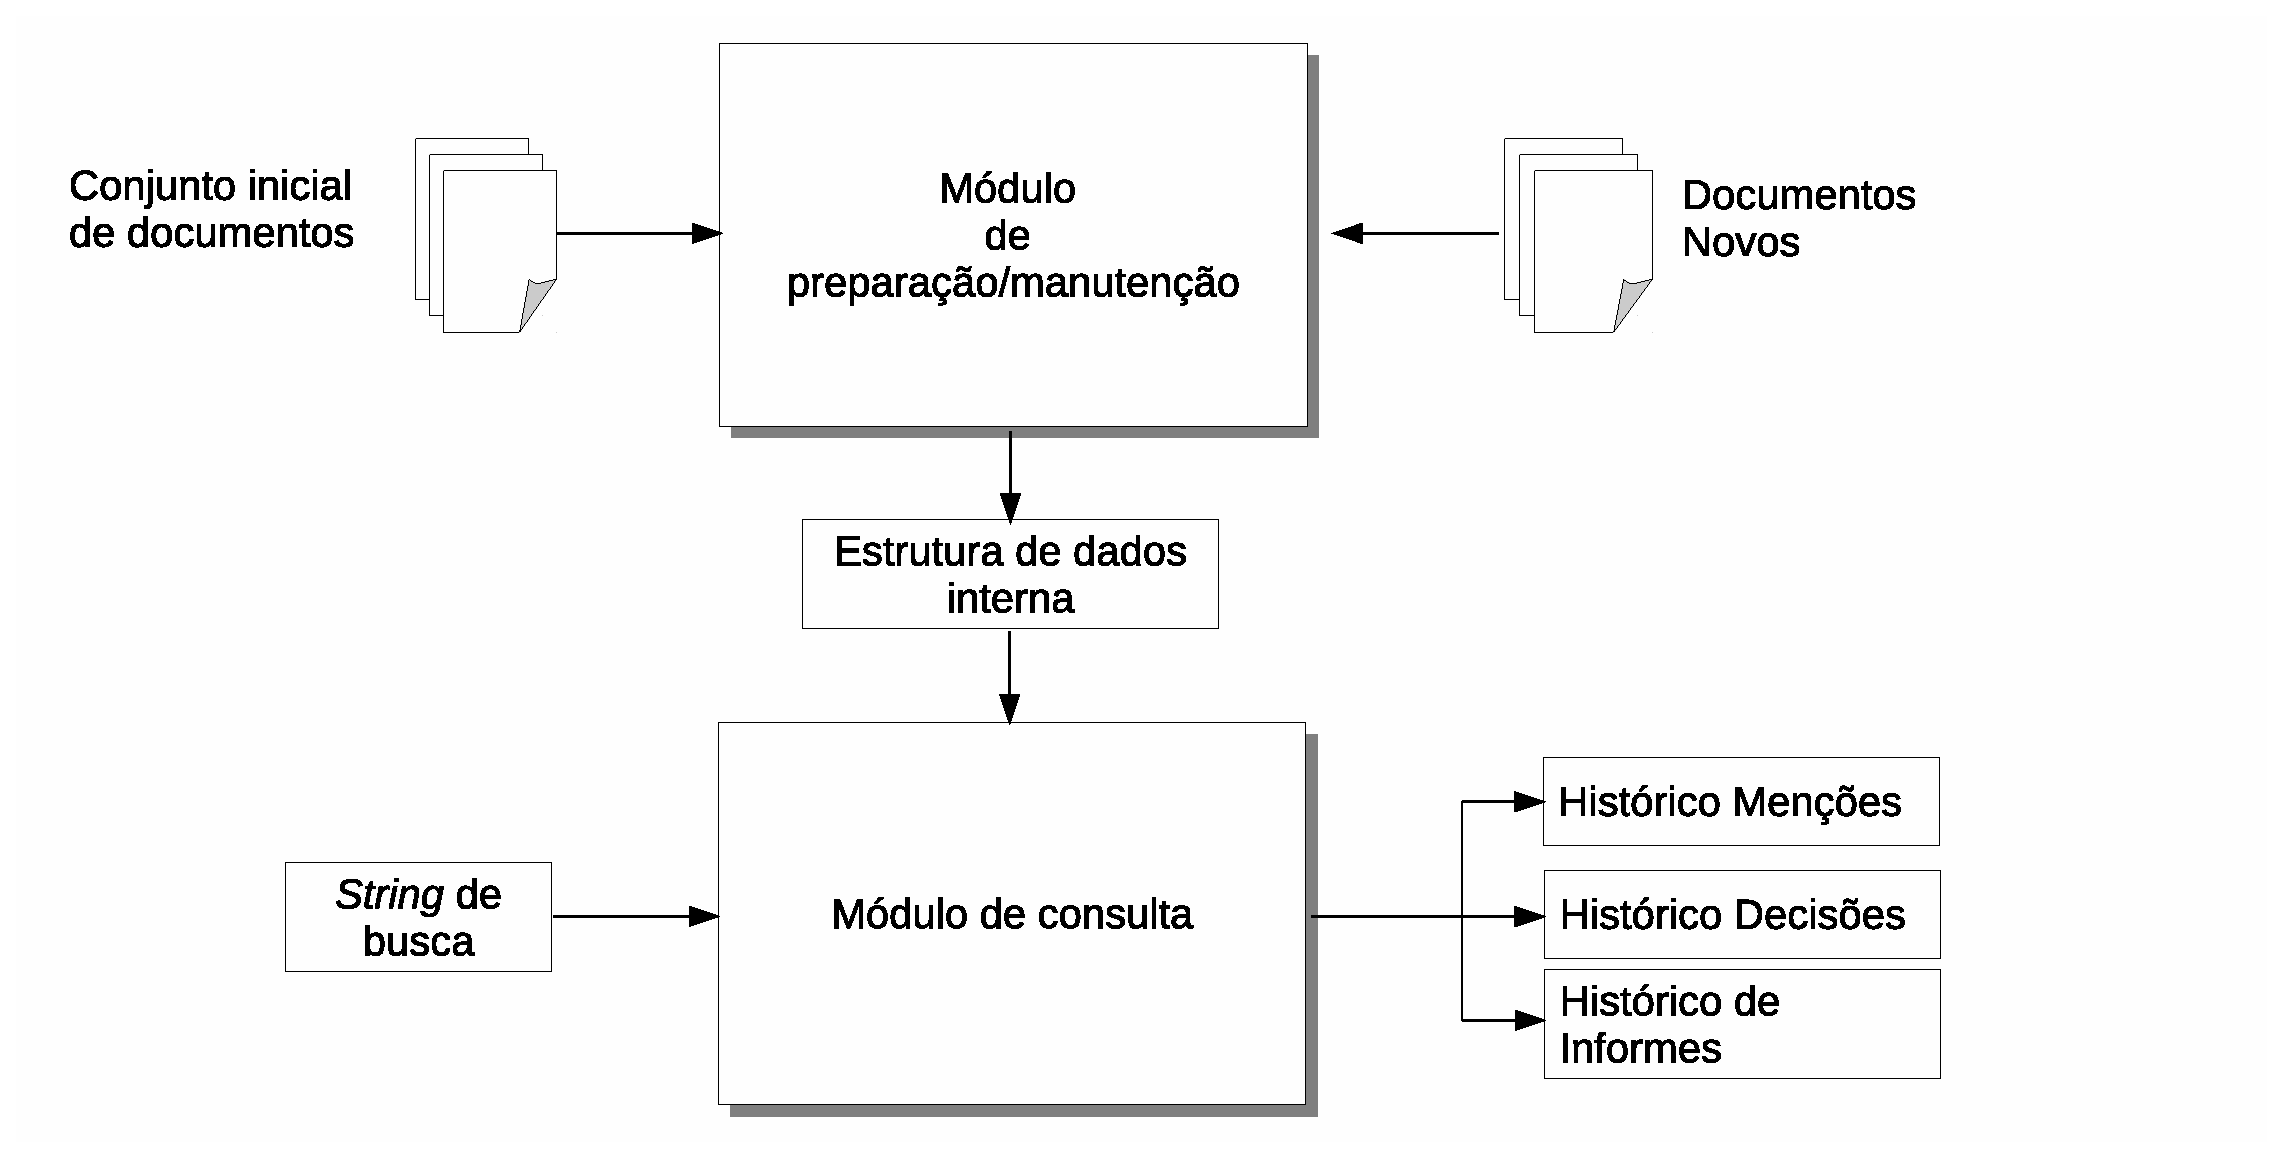
\includegraphics[width=0.69\paperwidth]{conteudo/capitulos/figs/visao-geral-3.eps}
	  \caption{Visão geral do sistema}
	  \label{fig:visao-geral}
  \end{figure}






\section{Módulo de preparação e manutenção}

O módulo de preparação e manutenção tem como funções principais dividir cada ata em em segmentos de texto que contêm um assunto predominante, e separá-los em categorias por meio de técnicas de extração tópicos e classificação. Além disso, produz uma estrutura de dados que registra quais assuntos foram tratados na reunião, bem como o trecho do documento onde é discutido.  
% melhorar ↓↓↓↓↓
% --> ↓↓  Texto introdutório  ↓↓
% --> ↓↓↓↓↓↓↓↓↓↓↓↓↓↓↓↓↓↓↓↓↓↓↓↓↓↓
A seguir são apresentadas as etapas do módulo de preparação e manutenção desde a preparação dos documentos até a entrega da estrutura interna ao módulo de consulta. 


\subsection{Preparação dos documentos}

As atas são normalmente armazenadas em arquivos binários do tipo \textit{pdf}, \textit{doc}, \textit{docx} ou \textit{odt}. As atas devem ser pré-processadas e estruturadas para que posam ser aplicados métodos de MI e RI. Inicialmente, o texto puro é extraído e passa por processos de transformação conforme apresentados a seguir.

A Figura~\ref{fig:exemplopreprocessamento} mostra a etapa de preparação de um documento em português que inclui a remoção de elementos menos significativos e a identificação de sentenças e segmentos.
	
% -<? Colocar aqui uma explicação do que é um segmento e uma sentença?

\begin{center}
	\begin{figure}

	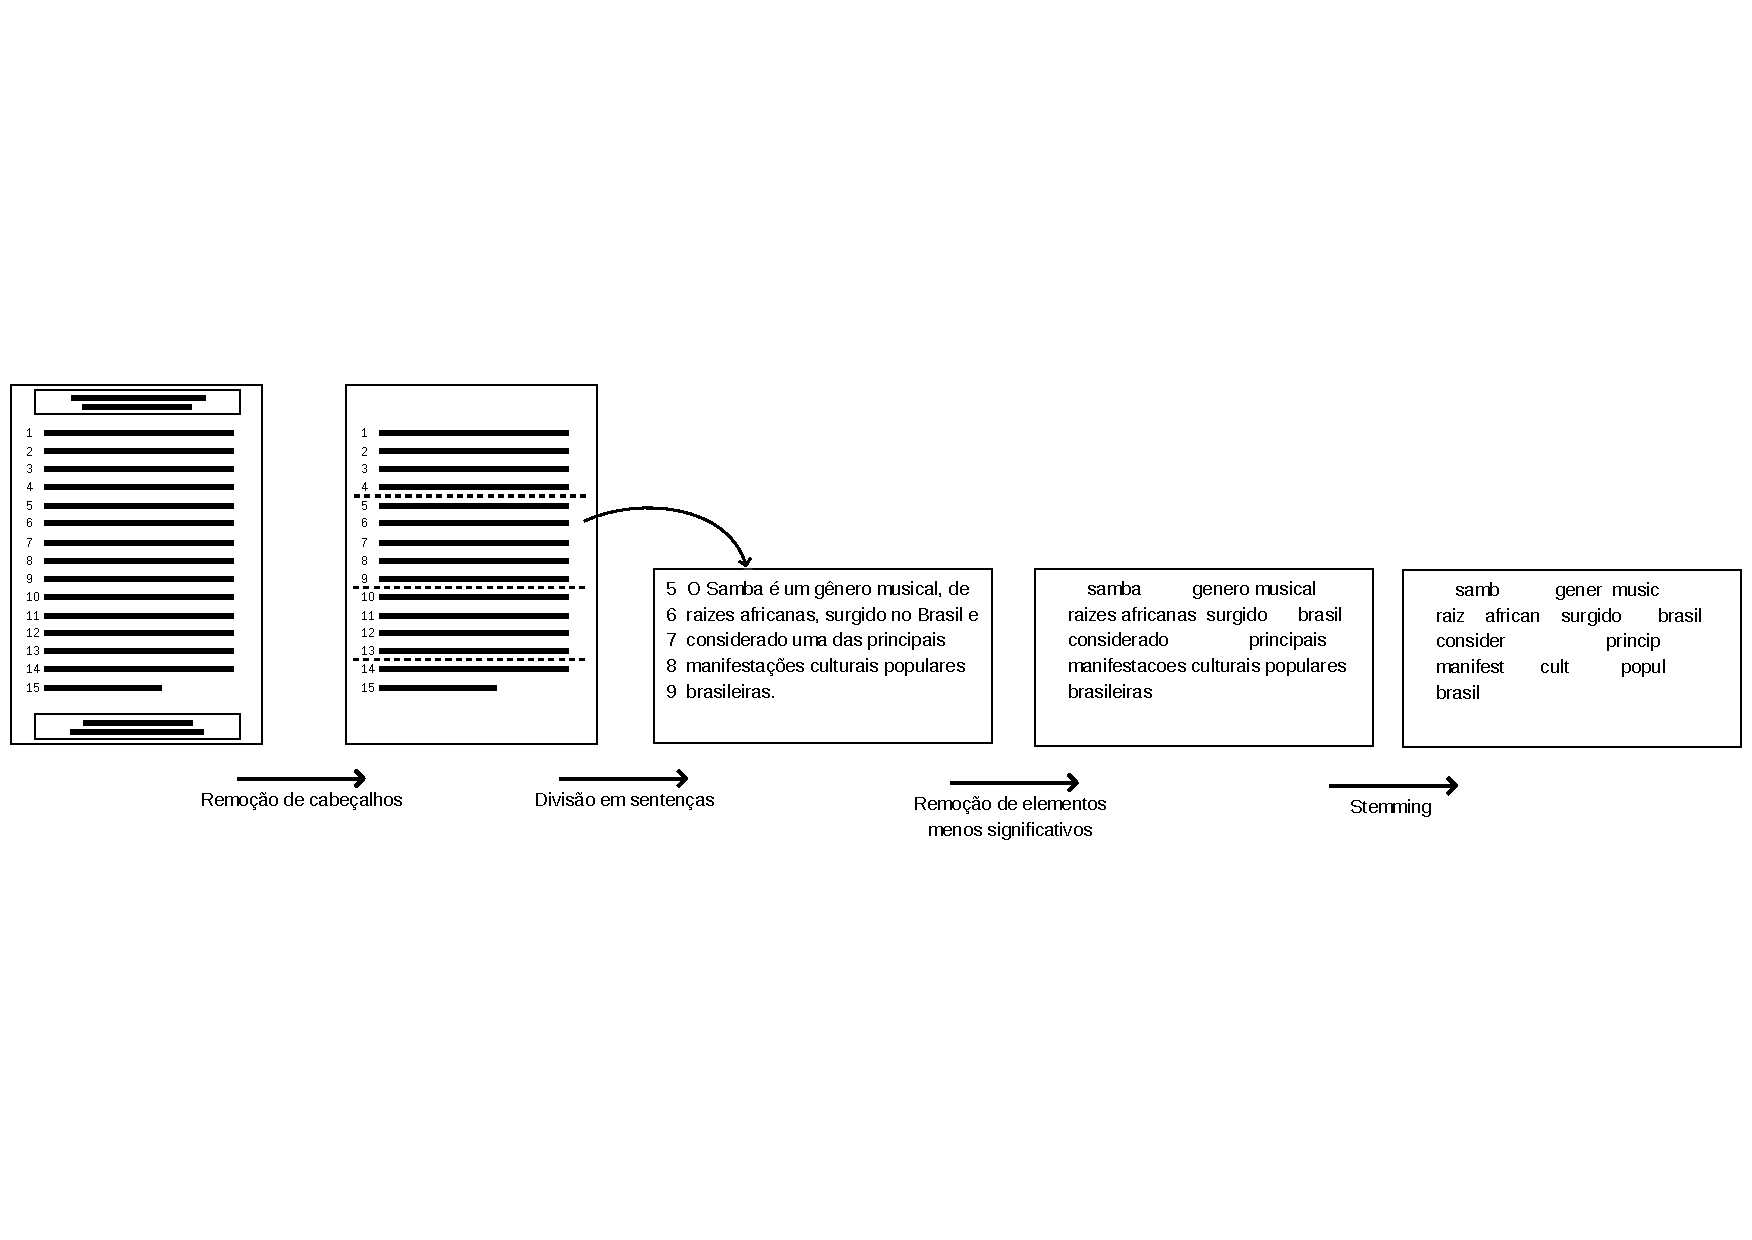
\includegraphics[trim={ 0 180 0 180 },clip,page=1,width=\textwidth]{conteudo/capitulos/figs/pre-process.pdf}

	\caption{Etapa de pré-processamento}
	\label{fig:exemplopreprocessamento}
	\end{figure}
\end{center}






\begin{enumerate}

%  Cabeçalhos e rodapés
\item Remoção de cabeçalhos e rodapés: as atas contém trechos que podem ser considerados pouco informativos e descartados durante o pré-processamento, como cabeçalhos e rodapés que se misturam aos tópicos tratados na reunião, podendo ser inseridos no meio de um tópico prejudicando tanto os algoritmos de MT e RI, quanto a leitura do texto pelo usuário. Um cabeçalho é a porção de texto que inicia cada página do documento e, de forma semelhante, um rodapé e a porção que as encerra. Detecta-se os cabeçalhos e os rodapés sempre que há uma repetição das primeiras e últimas palavras do documento.


%  Identificação de sentenças
\item Identificação de finais sentenças: Ao considerar intuitivamente que uma sentença seja uma sequência de palavras entre sinais de pontuação como ``.'', ``!'' e ``?'', alguns erros poderiam ocorrer quando esses tiverem outra função dentro do texto como em abreviações, endereços de internet e datas. Outro problema seriam frases curtas com poucas palavras e que não expressam um conceito completo, mas parte dele. Devido ao estilo de pontuação desses documentos, como encerrar sentenças usando um \textit{``;''} e inserção de linhas extras, foram usadas as regras especiais para identificação de finais de sentença. No Algoritmo~\ref{alg:identificacaofinaisdesent} é mostrado como cada \textit{token} é identificado e marcado com final de sentença.%, esse processo é melhor descrito na Subseção~\ref{subsec:indentificacaosentencas}. % Os detalhes sobre essas regras estão disponíveis para consulta em \urlsoftwares.



\begin{algorithm}
	\SetKwInOut{Input}{Entrada}
	\SetKwInOut{Output}{Saída}
	\SetKwBlock{Inicio}{início}{fim}
	\SetKwFor{ParaTodo}{para todo}{}{fim para todo}
	\SetKwIF{Se}{SenaoSe}{Senao}{}{}{senao se}{senao}{fim se}
	\SetKwFor{Para}{}{}{}
%	\SetKwAlgorithm{Algorithm}{Algoritmo}{}

	
	\Input{Texto}
	\Output{Texto com identificações de finais de sentença}
	
	\ParaTodo {token, marcá-lo como final de sentença se:} {	

	Terminar com um \texttt{!}\\
	Terminar com um \texttt{.} e não for uma abreviação\\
	Terminar em \texttt{.?;} e:
		\Para{}{
			For seguido de uma quebra de parágrafo ou tabulação\\
			O próximo \textit{token} iniciar com  \texttt{(\{["'}\\
			O próximo \textit{token} iniciar com letra maiúscula\\
			O penúltimo caracter  for \texttt{)\}]"'}\\
		}
	}
	
	\caption{Identificação de finais de sentença}
	\label{alg:identificacaofinaisdesent}
\end{algorithm}




%  Remoção de termos
\item Redução de termos: Removeu-se do as palavras que não contribuem para a distinção do texto em tópicos ou categorias, as quais são chamadas de \textit{stop words}. Palavras como artigos, preposições, pronomes, verbos de estado\footnote{Apresentam uma situação inativa, onde o verbo não expressa uma alteração, mas apenas uma propriedade ou condição dos envolvidos.}. Trata-se também como \textit{stop words} as palavras de uso muito frequente dentro de um determinado domínio as quais não são capazes de discriminar documentos, portanto também não devem fazer parte dos atributos~\cite{Rezende2003}. Para removê-las, as letras foram convertidas em caixa baixa e usou-se uma lista de 438 palavras para identificá-las. Além disso, eliminou-se a acentuação, sinais de pontuação, numerais e todos os \textit{tokens} menores que três caracteres.

%  Stemming
\item \textit{Stemming}: extraiu-se o radical de cada palavra. Para isso, aplicou-se o algoritmo \textit{Orengo} %\footnote{http://www.inf.ufrgs.br/~viviane/rslp/} 
	para remoção de sufixos~\cite{Alvares2005}.

\end{enumerate}
	


% -< Ao final .....



% ==================== Segmentação ===================== %


\subsubsection{Segmentação}

Como já mencionado, uma ata registra a sucessão de assuntos discutidos em uma reunião, porém apresenta-se com poucas quebras de parágrafo e sem marcações de estrutura, como capítulos, seções ou quaisquer indicações sobre o assunto do texto. Portanto, faz-se necessário descobrir quando há uma mudança de assunto no texto da ata. Para essa tarefa, as técnicas de segmentação de texto recebem uma lista de sentenças, da qual considera cada ponto entre duas sentenças como candidato a limite, ou seja, um ponto onde há transição entre assuntos~\cite{Bokaei2015, Bokaei2016, Misra2009, Sakahara2014}.


% Para esse trabalho, os algoritmos \textit{TextTiling} ~\cite{Hearst1994} e \textit{C99}~\cite{Choi2000} foram avaliados na tarefa de segmentação dos textos extraídos das atas conforme apresentado a seguir.

Entre os principais trabalhos da literatura podemos citar o \textit{TextTiling} ~\cite{Hearst1994} e o \textit{C99}~\cite{Choi2000} são considerados um dos primeiros mais influentes sendo utilizados com \textiit{base lines} em trabalhos recentes\cite{CHAIBI2014, Naili2016, Cardoso2017}

% --> CONTINUA ....


\subsubsection{Segmentação de Referência}
	 \label{subsubsec:segmetacaoreferencia}

 % \subsubsection{Avaliação dos Segmentadores}
 %  Critérios de avaliação
 Para que se possa avaliar um segmentador automático de textos é preciso uma referência, isto é, um texto com os limites entre os segmentos conhecidos. Essa referência, deve ser confiável, sendo uma segmentação legítima que é capaz de dividir o texto em porções relativamente independentes, ou seja, uma segmentação ideal.
% Como foram obtidas (software e especialistas) 
A fim de obter um conjunto de documentos segmentados que possam servir como referência na avaliação, os documentos coletados foram segmentados manualmente por dois coordenadores de curso que participam de reuniões. Para isso, utilizou-se um \textit{software}, desenvolvido com esse objetivo especifico, que permitiu aos voluntários visualizar um documento, e indicar livremente as divisões entre segmentos. Com o uso desse \textit{software} foram coletados os dados de seis atas segmentadas pelos participantes das reuniões, os quais serviram como referência para a avaliação dos algoritmos. O \textit{software} desenvolvido para segmentação manual está disponível para utilização e consulta em~\urlsoftwares	

Os arquivos gerados foram tratados para que os segmentos sempre terminem em uma sentença reconhecida pelo algoritmo, uma vez que as sentenças são a unidade mínima de informação nesse trabalho.

A Tabela~\ref{tab:segmentacaoreferencia} contém, para cada ata, a quantidade de sentenças e a quantidade de segmentos identificadas pelos participantes.



% Referência ····························································
% Documento	|	Segmentos Esp 1 |	Segmentos Esp 2
% Doc1		|	7 				|	15
% Doc2		|	9 				|	20
% Doc3		|	7 				|	15
% Doc4		|	9 				|	17
% Doc5		|	4 				|	9 
% Doc6		|	11				|	17
\begin{table}[!h]
	\centering
	\begin{tabular}{|l|c|c|c|} \hline
		\textbf{Ata} & \textbf{Sentenças}  & 
		\textbf{Participante 1}  & 
		\textbf{Participante 2} \\	\hline

		Ata 1 & 18 & 7  & 15 \\ \hline 
		Ata 2 & 26 & 9  & 20 \\ \hline 
		Ata 3 & 24 & 7  & 15 \\ \hline 
		Ata 4 & 32 & 9  & 17 \\ \hline 
		Ata 5 & 25 & 11 & 17 \\ \hline 
		Ata 6 & 10 & 4  & 9  \\ \hline 

	\end{tabular}
	\caption{Quantidade de sentenças e segmentos de referência por ata.}
	\label{tab:segmentacaoreferencia}
\end{table}




% --> Falar da coesão léxica peculiar das atas!!



\subsection{Configuração experimental}
	\label{subsec:configuracaoexperimental}

%%%%%%%%%%
% Parâmetros
%%%%%%%%%%
% As implementações dos algoritmos permitem ao usuário a configuração de seus parâmetros. 
%
O \textit{TextTiling} permite ajustarmos dois parâmetros, sendo o tamanho da janela e o passo. Por meio de testes empíricos escolheu-se os valores os valores 20, 40 e 60 para o tamanho da janela e 3, 6, 9 e 12 para o passo. Gerando ao final 20 configurações.
%

O \textit{C99} permite o ajuste de três parâmetros, sendo, o primeiro a quantidade segmentos desejados, uma vez que, não se conhece o número ideal de segmentos e os documentos não apresentam muitos candidatos, calculou-se uma proporção dos candidatos a limite. Para isso atribuiu-se os valores {0,2; 0,4; 0,6; 0,8}. O segundo parâmetro, o tamanho do quadro utilizado para gerar a matriz de ranking, atribuiu-se os valores 9 e 11, sendo 11 o valor padrão da apresentado pelo autor. O algoritmo permite ainda indicar se as sentenças serão representados por vetores contendo a frequência ou o peso de cada termo. Ambas as representações foram utilizadas. Considerando todos os parâmetros, foram geradas 16 configurações para o algoritmo \textit{C99}.





\subsubsection{Critérios de avaliação}

%%%%%%%%%%
% Definição do que é um bom algoritmo de segmentação
%%%%%%%%%%
Para fins de avaliação desse trabalho, um bom método de segmentação é aquele cujo resultado melhor se aproxima de uma segmentação manual, sem a obrigatoriedade de estar perfeitamente alinhado com tal. Ou seja, visto o contexto das atas de reunião, e a subjetividade da tarefa, não é necessário que os limites entre os segmentos (real e hipótese) sejam idênticos, mas que se assemelhem em localização e quantidade.


Os algoritmos foram comparados com a segmentação fornecida pelos participantes das reuniões. Calculou-se as medidas mais aplicadas à segmentação textual, P$_k$ e \textit{WindowDiff}. Além dessas, computou-se também as medidas tradicionais acurácia, precisão, revocação e $F^1$ para comparação com outros trabalhos que as utilizam.

Inicialmente, calculou-se as medidas configurando cada algoritmo conforme mostrado na Subseção~\ref{subsec:configuracaoexperimental}, sem aplicar o pré-processamento. O teste de Friedman com pós-teste de Nemenyi foi utilizado para gerar um ranking das melhores configurações para cada medida calculada. Com isso, foi possível descobrir quais valores otimizam um algoritmo para uma medida, 	desconsiderando o pré-processamento. 

A fim de conhecer o impacto do pré-processamento, repetiu-se os testes com o texto pré-processado. Com isso, descobriu-se quais valores otimizam os algoritmos para cada medida, considerando essa etapa.

Com os testes anteriores obteve-se, para cada medida, 4 configurações, levando em conta ambos os algoritmos e a presença ou ausência do pré-processamento. Novamente utilizou-se o teste de Friedman e Nemenyi e descobriu-se, para cada medida, qual configuração a otimiza. Os resultados completos estão disponíveis para consulta em~\urlsoftwares.




\subsubsection{Resultados}


Obteve-se, por meio dos testes estatísticos apresentados, as melhores configurações para as principais medidas de avaliação de segmentadores. Com essas configurações calculou-se a média de cada medida considerando o conjunto de documentos. Na Tabela~\ref{tab:resultadosTT} são apresentadas, as médias obtidas com o \textit{TextTiling} bem como as configurações utilizadas, onde \textbf{J} é o tamanho da janela e \textbf{P} é o passo.


\begin{table}[!h]
	\centering
	\begin{tabular}{|l||c|c|c||c|c|c|} \hline

		& \multicolumn{3}{c||}{Sem Pré-processamento} 
		& \multicolumn{3}{c|}{Com Pré-processamento}\\			

		\textbf{Medida} & 
		\textbf{J} &
		\textbf{P} & 
		\textbf{Média} &
		\textbf{J} &
		\textbf{P} & 
		\textbf{Média} \\	\hline

		P$_k$				& 50 & 9 & 0,142 & 50 & 9  & 0,144 \\ \hline
		\textit{WindowDiff}	& 50 & 6 & 0,387 & 40 & 9  & 0,396 \\ \hline
		Acurácia			& 50 & 6 & 0,612 & 40 & 9  & 0,603 \\ \hline
		Precisão			& 40 & 9 & 0,611 & 50 & 12 & 0,613 \\ \hline
		Revocação			& 20 & 3 & 0,886 & 20 & 3  & 0,917 \\ \hline
		F$^1$				& 30 & 6 & 0,605 & 40 & 3  & 0,648 \\ \hline

	\end{tabular}
	\caption{Resultados obtidos com o \textit{TextTiling}}
	\label{tab:resultadosTT}
\end{table}




Na Tabela~\ref{tab:resultadosc99} são apresentadas, as médias obtidas com o \textit{C99} bem como as configurações utilizadas, onde \textbf{S} é a proporção de segmentos em relação a quantidade de candidatos, \textbf{M} é o tamanho do quadro utilizado para criar a matriz de \textit{rankings} e \textbf{W} indica se os segmentos são representados por vetores contendo a frequência ou um peso das palavras.


\begin{table}[!h]
	\centering
	\begin{tabular}{|l||c|c|c|c||c|c|c|c|} \hline

		& \multicolumn{4}{c||}{Sem Pré-processamento} 
		& \multicolumn{4}{c|}{Com Pré-processamento}\\			

		\textbf{Medida} & 
		\textbf{S} & 
		\textbf{M} & 
		\textbf{W} & 
		\textbf{Média} &
		\textbf{S} & 
		\textbf{M} & 
		\textbf{W} & 
		\textbf{Média} \\	\hline

		P$_k$				& 20 & 9 & Sim & 0,134& 20 & 11 & False	& 0,116 \\ \hline  
		\textit{WindowDiff}	& 60 & 9 & Sim & 0,411& 60 &  9 & Sim 	& 0,390 \\ \hline  
		Acurácia			& 60 & 9 & Sim & 0,588& 60 &  9 & Sim 	& 0,609 \\ \hline  
		Precisão			& 40 & 9 & Sim & 0,645& 20 & 11 & False	& 0,720 \\ \hline  
		Revocação			& 80 & 9 & Sim & 0,869& 80 & 11 & Sim 	& 0,897 \\ \hline  
		F$^1$				& 80 & 9 & Sim & 0,638& 80 & 11 & Sim 	& 0,655 \\ \hline  

	\end{tabular}
	\caption{Resultados obtidos com o \textit{C99}}
	\label{tab:resultadosc99}
\end{table}




De acordo com os últimos testes, o algoritmo \textit{C99} obteve melhor desempenho em acurácia, precisão, $F^1$, $P_k$ e \textit{WindowDiff}, enquanto o \textit{TextTiling} obteve o melhor desempenho em revocação como pode ser visto na Tabela~\ref{tab:configfinal}. 







% O algoritmo \textit{C99} obteve melhor desempenho em acurácia, precisão, $F^1$, $P_k$ e \textit{WindowDiff}, enquanto o \textit{TextTiling} obteve o melhor desempenho em revocação como pode ser visto na Tabela~\ref{tab:configfinal}. 


% \begin{table}[!h]
	% \centering

	% \begin{tabular}{|l|l|c|c|c|c|c|} \hline
		% \textbf{Algoritmo} & 
		% \textbf{Medida} & 
		% \textbf{Média}\\	\hline

	% \textit{C99} & P$_k$			   & 0,116 \\ \hline
	% \textit{C99} & \textit{WindowDiff} & 0,390 \\ \hline
	% \textit{C99} & Acurácia			   & 0,609 \\ \hline
	% \textit{C99} & Precisão			   & 0,720 \\ \hline
	% \textit{C99} & F$^1$			   & 0,655 \\ \hline
	% \textit{TextTiling} &	Revocação  & 0,917 \\ \hline

	% \end{tabular}
	
	% \caption{Melhores resultados obtidos.}
	% \label{tab:configfinal}
% \end{table}




\begin{table}[!h]
	\centering
\begin{tabular}{|l||c|c|c|c|c|c|c|} 
\hline 
\textbf{M\'{e}todo} & 
\textbf{Pk} & 
\textbf{WD} & 
\textbf{A } & 
\textbf{P } & 
\textbf{R } & 
\textbf{F1} & 
\textbf{Segmentos}\\ \hline

Senten\c{c}as & 0.320 & 0.502 & 0.498 & 0.498 & \textbf{1.000} & \textbf{0.642} & 22.083\\ \hline
TextTiling    & 0.275 & 0.469 & 0.531 & 0.514 & 0.937 & 0.640 & 19.583\\ \hline
C99           & 0.142 & 0.426 & 0.574 & 0.601 & 0.473 & 0.506 & 8.167\\ \hline
BayesSeg      & 0.148 & 0.414 & 0.586 & 0.599 & 0.526 & 0.528 & 8.750\\ \hline
MinCut        & 0.226 & 0.532 & 0.468 & 0.464 & 0.438 & 0.432 & 10.333\\ \hline
TextSeg       & \textbf{0.085} & \textbf{0.387} & \textbf{0.613} & \textbf{0.714} & 0.412 & 0.497 & 5.167\\ \hline
\end{tabular} 

	\caption{Melhores resultados obtidos.}
	\label{tab:configfinal}
\end{table}









%  we have a winner
Verificou-se que, de maneira geral, o algoritmo \textit{C99} apresenta melhores resultados em relação ao \textit{TextTiling}, contudo, testes estatísticos realizados indicaram que não houve diferença significativa entre os métodos. Nesse trabalho, escolheu-se o algoritmo \textit{C99} por apresentar resultados satisfatórios e ligeira superioridade em relação ao \textit{TextTiling}. 






% cada segmento é um documento
Após a identificação dos segmentos, o algoritmo retorna uma lista onde cada elemento é um texto com um assunto predominante e será a partir de disso considerado um documento.

% -? Medidas

% -- como ele faz?




%  ==========   ==========   ==========   ==========   ==========   

\subsection{Representação Computacional}

As etapas anteriores produzem fragmentos de documentos onde o texto esta em um estágio de processamento inicial, com menos atributos que as versões originais, onde cada fragmento está associado a um tema, porém, ainda não estruturado. Ocorre que as técnicas de mineração de texto exigem uma representação estruturada dos textos. % conforme será visto na Seção~\ref{subsection:RepTextos}.

Uma das formas mais comuns é a representação no formato matricial conhecida como Modelo Espaço Vetorial (\textit{Vectorial Space Model} - VSM)~\cite{Rezende2003}, onde os documentos são representados como vetores em um espaço Euclidiano $t$-dimensional em que cada termo extraído da coleção é representado por um dimensão. Assim, cada componente de um vetor expressa a relação entre os documentos e as palavras. Essa estrutura é conhecida como \textit{document-term matrix} ou matriz documento-termo.

A forma adotada nesse trabalho é a \textit{Bag Of Words} a qual sintetiza a base de documentos em um contêiner de palavras, ignorando a ordem em que ocorrem, bem como pontuações e outros detalhes, preservando apenas o peso de determinada palavra nos documentos. É uma simplificação de toda diversidade de informações contidas na base de documentos sem o propósito de ser uma representação fiel do documento, mas oferecer a relação entre as palavras e os documentos a qual é suficiente para a maioria dos métodos de aprendizado de máquina.%~\cite{Rezende2003}. 

% será empregada por ser a mais utilizada e referenciada na literatura e por sua simplicidade e qualidade dos resultados que são obtidos. 





\subsection{Extração de Tópicos / Classificação de Textos}

% a tarefa é identificar qual assunto está presente em cada trecho e qual é o tipo de ocorrência.



\section{Módulo Consulta}

Uma vez que a estrutura de dados interna contem os assuntos abordados na coleção de documentos, o tipo de ocorrência para cada assunto e o trecho onde se encontram, caberá ao módulo de consulta receber a \textit{string} de consulta do usuário, resgatar os dados desejados e apresentá-los em ordem cronológica, dando condições para o usuário acessar os segmentos encontrados bem como os documentos originais.

\subsection{Seleção dos tópicos}

\subsection{Visualização}

O usuário final precisa de uma interface adequada para visualizar os resultados da busca considerando-se a relevância dos tópicos selecionados e a sequência cronológica.

Uma boa apresentação deve permitir ao usuário identificar a relevância os resultados e ser relativante independente para compreensão do conteúdo, evitando a leitura do texto completo. Ou seja, o texto de cada tópico apresentado deve ser suficiente para compreensão do assunto mencionado, sem necessidade de visualizar o documento original.

As informações apresentadas, incluem dados obtidos do documento como o nome do arquivo e data do original e o texto onde o assunto é mencionado. Além disso, apresenta-se as informação extraídas pelas técnicas de mineração de texto como os descritores e rótulos.

% o sistema traz vários resultados para uma consulta, alguns mais relevantes que outros. Para cada resultado (que podem tratar de coisas diferentes) o sistema apresenta um histórico de menções para aquele assunto;

Para cada busca, é retornada uma lista de resultados ordenados pela relevância com a \textit{string} de entrada, sendo cada item referente a uma menção a um assunto. Um tópico é abordado em diferentes momentos e registrado em atas distintas, onde cada menção é um resultado a ser apresentado. 

Como parte da proposta, o sistema apresenta cada resultado dentro de um histórico de menções. Para isso, abaixo do texto é exibida uma linha com links para os resultados que compartilham o mesmo tópico ordenados por data. Os links, ao ser acionado, direciona para o resultado que aponta, além disso, quando o cursor do mouse está sobre o link, é apresentado um pre-visualização do texto. Dessa forma o usuário tem acesso uma interface que lhe fornece uma visão temporal das menções.

% Uma vez que um item faz menção a um tópico específico, 


% um histórico de menções para o assunto pesquisado.
% O sistema também apresenta junto com cada resultado, 


\section{Estudo de caso}
% -- qual o ganho em relação a um sitema de busca por palavras-chave? 


\section{Avaliação}


\chapter{Avaliação dos Segmentadores}\label{cap-segmentadores}




Nesse capítulo é apresentado uma análise dos algoritmos de segmentação textual com objetivo de iniciar uma discussão sobre a potencialidade das técnicas a serem utilizadas em um corpus constituído de atas de reuniões conforme já mencionado na Seção~\ref{subsec:composicaocorpus}. 
Os algoritmos \textit{TextTiling} e \textit{C99} são analisados deviso a sua abordagem linguística baseada em coesão léxica e por estarem entre os primeiros trabalhos nessa área e serem frequentemente referenciados até hoje~\cite{AlemiG15}. 
%	
Selecionou-se também os algoritmos \textit{BayesSeg} e \textit{TextSeg} por trazerem abordagens probabilísticas e o \textit{MinCutSeg} o qual é baseado em particionamento de grafos.
% 
Com além disso, incluiu-se também um algoritmo que simplesmente atribui um segmento a cada sentença chamado \textit{Sentenças} para fins de comparação com as técnicas anteriores.


Aqui será detalhada uma avaliação objetiva em que os resultados dos algoritmos foram avaliados por sua similaridade com uma segmentação de referência construída com base n metodologia de anotações em sub-tópicos proposta em~\cite{Hovy2010}. Em seguida escolheu-se um modelo que apresenta melhores resultados para ser utilizado em conjunto com técnicas de extração de tópicos em um experimento onde se avaliou a performance de ambas as técnicas junto a profissionais com afinidade com atas de reunião que forneceram suas percepções em relação aos resultados do segmentador empregado nesse trabalho. Os dados obtidos dos experimentos serviram de base para as análises dos algoritmos e de sua aplicação no contexto das atas de reuniões.




% ----- Segmnetação de Referência -----
A avaliação objetiva de um segmentador automático de textos exige uma referência, isto é, um conjunto de textos com os limites entre os segmentos conhecidos. Essa referência, deve ser confiável, sendo uma segmentação legítima que é capaz de dividir o texto em porções relativamente independentes, ou seja, uma segmentação ideal.
Optou-se por criar um \textit{corpus} de atas de reunião anotadas a fim de produzir-se uma segmentação de referência para avaliações dos algoritmos, bem como sua publicação e utilização em outros trabalhos voltados a esse domínio. A o processo de anotação e criação da segmentação de referência está detalhada nas próximas seções.


% =========== Avaliação dos Segmentadores ============ %
% \subsection{Avaliação dos Segmentadores}

\section{Preparação de um corpus de referência}




% ----- Anotação -----
A condução desse experimento teve como guia a metodologia apresentada em~\cite{Hovy2010} a qual indica sete passos para obter um corpus anotado. Essa metodologia está descrita a partir da Seção~\ref{subsec:anotacoes} e abordada com mais detalhes em~\cite{Cardoso2017}. 



% -- 1 - Escolha do Corpus
% O autor da metodologia indica que 
% Inicialmente, escolheu-se como \textit{corpus} a ser anotado	
O processo de anotação iniciou-se com a seleção de 12 atas de reunião do departamento de computação da UFSCar campus Sorocaba, as quais são disponibilizadas publicamente\footnote{Acessível em ppgccs.net\\ }. As atas foram coletadas dos departamentos de graduação e pós-graduação referentes a reuniões ordinárias e extraordinárias, a fim de selecionar documentos levando em conta a variedade em volume de texto e diversidade de assuntos abordados.

% -- 2 - Escolha da teoria a ser explicada
O trabalho de anotação, visa entender como usuários entendem as transições de assunto no documento, visto a ausência de marcações e meta informações no texto. Além disso, as anotações desse trabalho devem registrar o entendimento dos usuários em relação aos assuntos de cada segmento identificado e classificá-los quanto ao tipo de menção dada ao assunto. Maiores detalhes sobre a segmentação e rotulação manual serão fornecidos mais adiante nessa seção.
% do assunto como decisão, informe, irrelevante
% Com essas anotações pretende-se explicar como os usuários entendem a segmentação e lhes atribui tópicos.


% -- 3 - Selecionar e treinar os anotadores 
% -- 5 - Modelar uma interface para anotação
Após a delimitação do fenômeno a ser explicado e escolha do \textit{corpus} apropriado, selecionou-se um grupo de anotadores para analisar e coletar dados referentes a cada ata. O grupo de anotadores foi formado por profissionais com alguma afinidade com atas de reunião, como profissionais administrativos, professores e coordenadores de curso. 
A fim de facilitar o trabalho de anotação e diminuir eventuais erros, optou-se por desenvolver um \textit{software}\footnote{Códigos fontes disponíveis em: \url{https://github.com/ovidio-francisco/UFSCar/tree/master/codes/TextSegmentationTool} } como ferramenta para a coleta dos dados, conforme sugerido por~\cite{Hovy2010}. Essa ferramenta foi modelada para permitir aos anotadores visualizar os documentos e indicar livremente as divisões entre segmentos, bem como rotulá-los. 

Nesse processo, rotulou-se o assunto tratado no seguimento em 3 passos:
(1) classificação quanto ao tipo de comunicação, onde se especificou uma entre as classes 
\textit{``decisão``},
\textit{``informe''},
\textit{``irrelevante''} e 
\textit{``outro''} sendo que para essa última, o anotador poderia especificar livremente a classe.
(2) classificação quanto ao ao contexto onde se gerou o assunto, onde as classes, 
\textit{``discussão''},
\textit{``orientação''},
\textit{``solicitação''} e 
\textit{``outro''} podendo o anotador indicá-las simultaneamente.
(3) descrição do assunto, onde o anotador apontou até 5 palavras contidas no texto para representar o teor do segmento.

De acordo com a literatura a respeito de anotações em sub-tópicos, é recomendável fornecer treinamento aos participantes. Nesse trabalho os anotadores receberam apenas informações básicas sobre o objetivo da pesquisa e instruções de como operar o \textit{software} por meio de um vídeo\footnote{Acessível em }, deixando o entendimento sobre a segmentação e rotulação a critério do entendimento de cada anotador. Assim, nenhum critério foi estabelecido para o procedimento ficando os anotadores orientados apenas pela interface da ferramenta. Na Figura~\ref{fig:interfaceanotacoes} é mostrada a interface da ferramenta utilizada para as anotações.

  \begin{figure}[!h]
	  \centering
	  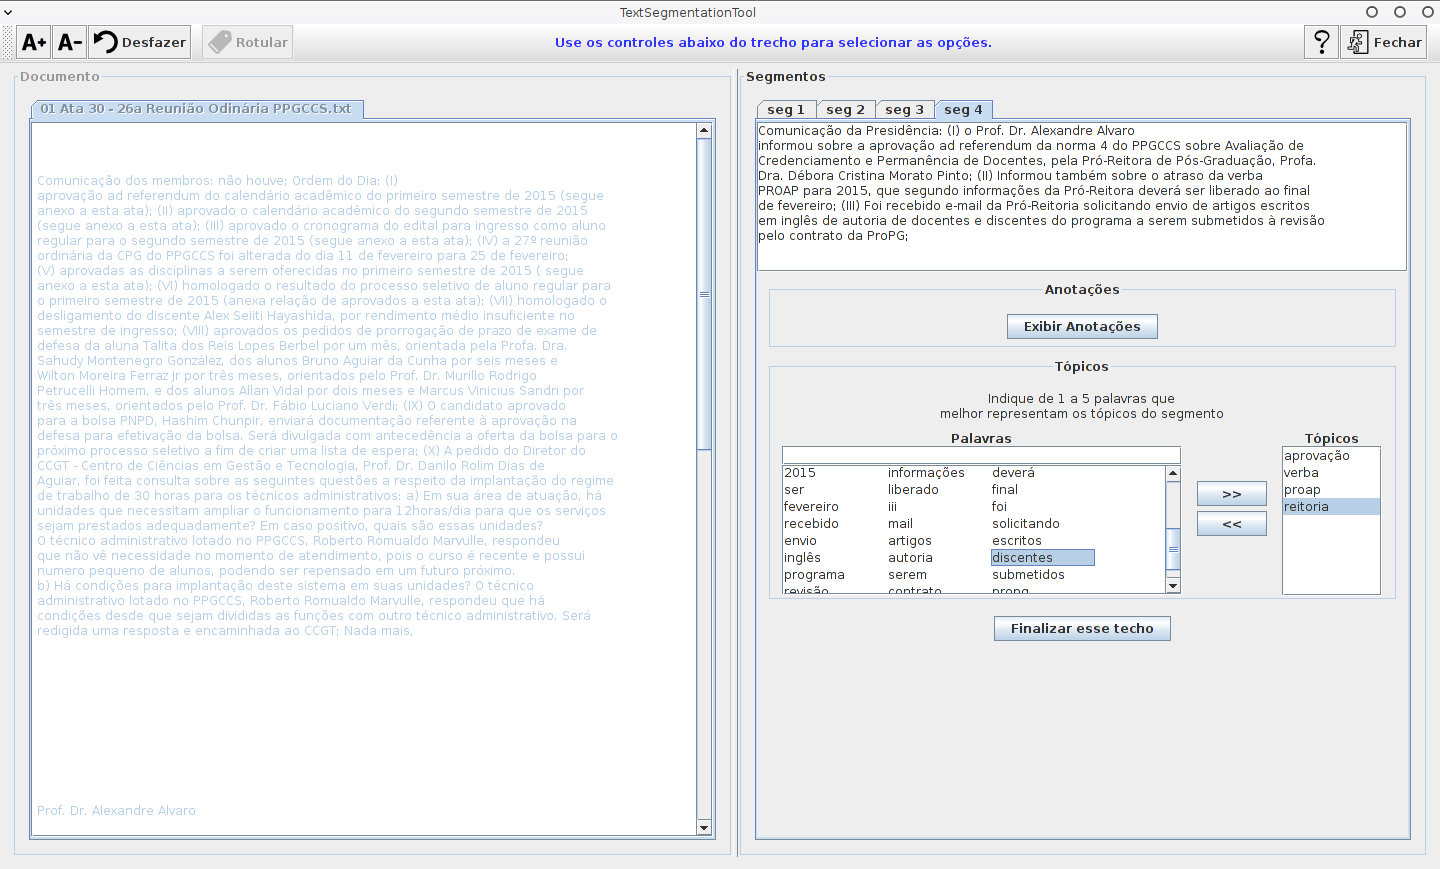
\includegraphics[width=1\textwidth]{conteudo/capitulos/figs/interface-anotacoes.png}
	  \caption{Interface da ferramenta utilizada para anotações onde o texto a ser segmentado é exibido no painel a esquerda e os controles para anotação estão disponíveis a direita.}
	  \label{fig:interfaceanotacoes}
  \end{figure}



% -- 4 - Especificar o procedimento de anotação
O procedimento de anotação deu-se remotamente, em que os anotadores receberam por e-mail o acesso ao \textit{software} e individualmente realizaram as anotações. A tarefa de segmentar e rotular manualmente demandou em torno de 4 a 6 horas de atenção dos anotadores. Em razão desse esforço, o \textit{software} permitiu que a tarefa fosse pausada e reiniciada sempre que houvesse necessidade, sem prejuízos ao trabalho.



% Os arquivos gerados foram tratados para que os segmentos sempre terminem em uma sentença reconhecida pelo algoritmo, uma vez que as sentenças são a unidade mínima de informação nesse trabalho.
O \textit{corpus} anotado deve ser constituído a partir dos textos originais e da resultante das percepções dos anotadores a certa do fenômeno a ser explicado. Assim, o texto de cada uma das 12 atas selecionadas será acrescido de informação gerada a partir dos dados coletados. Após o processo de anotação, a segmentação de referência foi criada utilizando o critério de maior concordância, como já relatado em outros trabalhos~\cite{Hearst1997, Cardoso2017, Kazantseva2012, Passonneau1997, Galley2003}. Considerou-se que ocorre um limite entre segmentos quando a maioria dos anotadores (metade mais um) concordou que a mesma sentença é um final de segmento. 

Na Figura~\ref{fig:concordanciasegref} é mostrado um exemplo de criação de uma segmentação de referência por meio da concordância entre anotadores. As primeiras linhas representam segmentações fornecidas por anotadores e a última linha representa a segmentação resultante da concordância entre a maioria dos segmentadores e portanto mais confiável. 

  \begin{center}
	\begin{figure}[h!]

	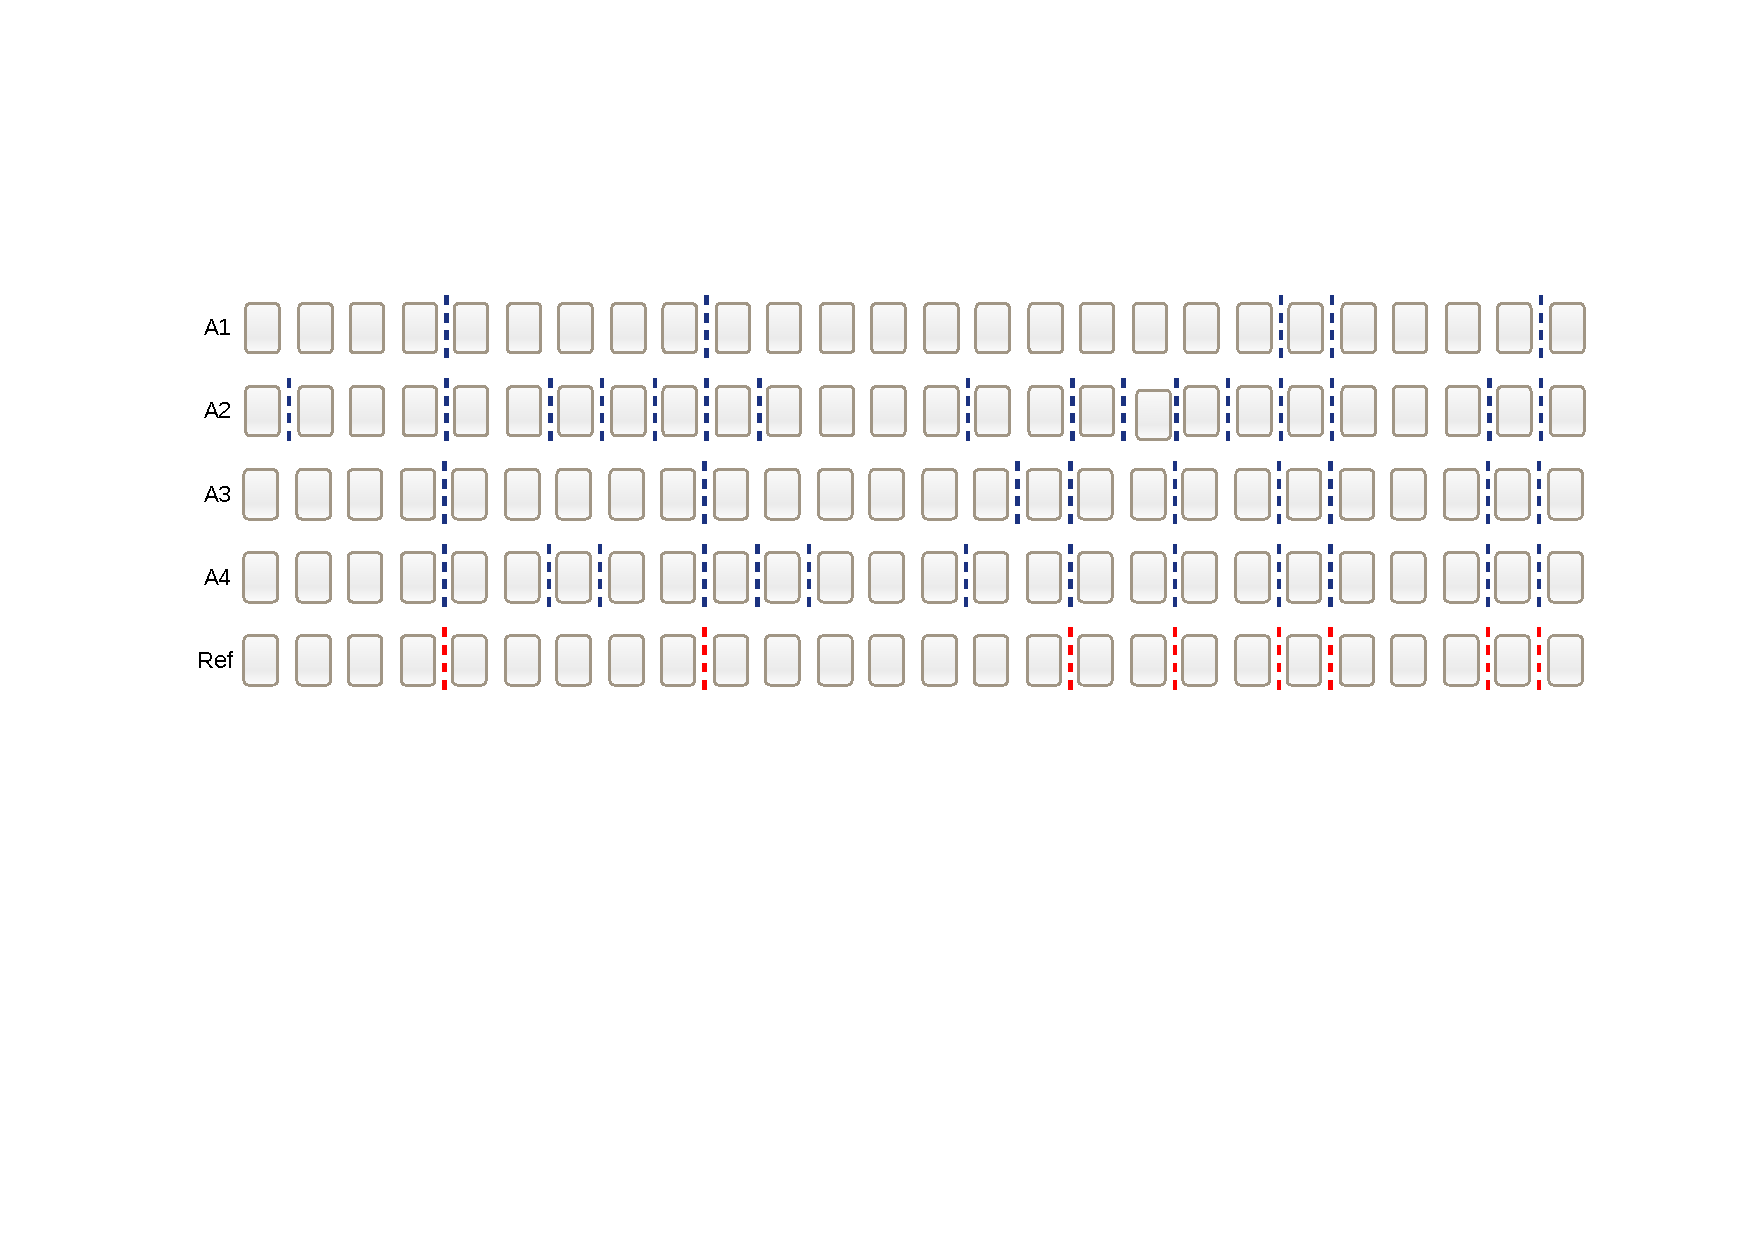
\includegraphics[trim={ 95 255 75 140 },clip,page=1,width=\textwidth]{conteudo/capitulos/figs/segmentacao-referencia.pdf}

	\caption{Exemplo uma segmentação de referência criada a partir da concordância entre segmentações manuais.}
	\label{fig:concordanciasegref}
	\end{figure}
\end{center}







% ----------------- Exemplo Segmentação de Referência ----------------------

Na Tabela~\ref{tab:segmentacaoreferencia} é mostrado um exemplo em que 6 dos 9 anotadores concordaram a respeito de um segmento. A tabela mostra quatro segmentos extraídos da segmentação de referência onde cada linha contém um segmento e os índices a esquerda indicam uma sentença. Junto à cada segmento é mostrado uma amostra das classes e descritores rotulados por um dos anotadores. Vale ressaltar que esses rótulos não foram utilizados no processo de segmentação e não têm nenhuma influência sobre a segmentação de referência. Nesse trabalho, essas anotações são utilizadas na avaliação dos extratores de tópicos.

\begin{table}[!h]
	\centering 
\footnotesize
% \scriptsize
	\begin{tabular}{|p{0.2cm}p{14,5cm}|} \hline


$^{[7]}$&
(II) Encerrada a etapa de inscrição para o processo seletivo como aluno regular para o segundo semestre de 2015: foram quarenta e nove inscrições on-line e dezoito candidatos entregaram a documentação; 
\textit{<informe>} \textit{<processo;seletivo>}
\\ \hline


$^{[8]}$ &
(III) O Prof. Dr. AAA informou que a Pró-Reitora comunicou a oferta de mais uma bolsa pela cota da Pró-Reitoria, mas não havia aluno disponível para alocação da bolsa.\\
$^{[9]}$ &
(III) O Prof. Dr. AAA informou que a Pró-Reitora comunicou a oferta de mais uma bolsa pela cota da Pró-Reitoria, mas não havia aluno disponível para alocação da bolsa.\\
$^{[10]}$ &
O Prof. Dr. BBB informou que havia uma aluna interessada, mas não informada durante o processo de elaboração do ranking no início do semestre.\\
$^{[11]}$ &
Ficou decidido enviar e-mail aos docentes solicitando que comuniquem permanentemente interesse de alunos em bolsa pra atualização do ranking;
\textit{<informe>} \textit{<solicitação;bolsa;cota;ranking;alunos>}
\\ \hline


$^{[12]}$ &
(IV) Com a mudança do Prof. Dr. DDD para o campus de São Carlos, o Prof. Dr. BBB assume o posto de suplente da linha Teoria Aplicada à Computação na CPG;
\textit{<informe>} \textit{<mudança;suplente;teoria;aplicada;computação>}
\\ \hline

$^{[13]}$ &
	Comunicação dos membros: Não houve;
	\textit{<irrelevante>} 
\\ \hline



% $^{[14]}$ &
% Ordem do Dia: (I) Foram apresentadas regras para participação de membro externo em banca de defesa do mestrado.\\
% $^{[15]}$ &
% O Prof. Dr. Alexandre Alvaro comentou que está sendo pago aos participantes externos das bancas a diária pelo PROAP e o pró-labore pelo DComp, além do programa fornecer o transporte, que onera a verba PROAP.\\
% $^{[16]}$ &
% O Prof. Dr. Tiago Agostinho de Almeida sugeriu o seguinte cálculo para pagamento: se o participante vier de uma Instituição com distância até 220 km será feito o cálculo de R\$ 1,00 multiplicado pela quilometragem.\\
% $^{[17]}$ &
% Caso a distância seja superior a 220 km, será calculada a distância multiplicada por R\$ 0,60. O menor valor entre o custo do transporte e o pagamento de verba e pró-labore será utilizado para custear a vinda do participante;
% \\ \hline



% $^{[18]}$ &
% (II) Foi discutida a forma de convalidação de disciplinas cursadas como aluno regular anterior a três anos do reingresso do aluno.
% Foi decidido que fica a cargo da CPG decidir sobre as disciplinas que serão aproveitadas quando do reingresso do aluno;
% \\ \hline



% $^{[13]}$ &

	\end{tabular}
	\caption{Exemplo de segmentação de referência com rotulação de um anotador}
	\label{tab:segmentacaoreferencia}
\end{table}









  




% -- 6 - Escolher e aplicar medidas de avaliação
Para mensurar a concordância entre anotadores, a medida \textit{kappa (k)}~\cite{Carletta1996} é frequentemente utilizada~\cite{Gruenstein2007, Cardoso2017, Hearst1997}. Ela mostra como os anotadores compreendem os textos analisados e o nível de confiabilidade da segmentação de referência. Essa medida retorna um valor no intervalo de 0 até 1, onde 1 significa uma concordância perfeita e 0 que não houve concordância. 
% As medidas de similaridade entre segmentações também podem ser utilizadas para avaliar a qualidade da segmentação de referência. 
As medidas \textit{WindowDiff} e $P_k$ informam a probabilidade de duas sentenças escolhidas aleatoriamente estarem no mesmo segmento. Elas refletem a similaridade entre duas segmentações, assim também podem ser utilizadas para avaliar a concordância entre os anotadores. As formulações dessas medidas são abordadas em mais detalhes na Seção~\ref{subsec:medidas-segmentacao}.
Nesse trabalho, para cada segmentação fornecida por cada anotador calcula-se as medidas \textit{WindowDiff}, $P_k$ e \textit{Kappa}.
A Tabela~\ref{tab:ataseanotacoes} contém, para cada ata, a quantidade de sentenças e a quantidade de segmentos identificadas pelos participantes e as médias de \textit{WindowDiff}, $P_k$ e \textit{Kappa}. Uma vez que P$_k$ e \textit{WindowDiff}, são medidas de dissimilaridade, são reportados os seus complementos.
% Uma vez que P$_k$ e WD, indicam melhores valores próximos a 0 e 1 como dissimilarid 

\begin{table}[!h]
	\centering
	\begin{tabular}{|l|c|c|c|c|c|c|c|c|c|c|c|c|c|} \hline
		\textbf{Ata} & \textbf{Sent.}  & 
		\textbf{A1}  & 
		\textbf{A2}  & 
		\textbf{A3}  & 
		\textbf{A4}  & 
		\textbf{A5}  & 
		\textbf{A6}  & 
		\textbf{A7}  & 
		\textbf{A8}  & 
		\textbf{A9}  &
		\textbf{k}  &
		\textbf{P$_k$}  &
		\textbf{WD}  \\	\hline

% 		              A1   A2   A3  A4    A5   A6   A7   A8   A9   
		Ata 1  & 25 & 7  & 4  & 11 & 6  & 16 & 8  & 8  & 15 & 16 &  0.344 & 0.593 & 0.475 \\ \hline 
		Ata 2  & 17 & 4  & 4  & 8  & 6  & 11 & 6  & 6  & 15 & 14 &  0.377 & 0.572 & 0.509 \\ \hline 
		Ata 3  & 26 & 6  & 6  & 8  & 4  & 15 & 9  & 10 & 18 & 14 &  0.384 & 0.603 & 0.524 \\ \hline 
		Ata 4  & 26 & 5  & 5  & 10 & 6  & 14 & 17 & 7  & 11 & 12 &  0.447 & 0.652 & 0.540 \\ \hline 
		Ata 5  & 33 & 4  & 4  & 6  & 5  & 17 & 22 & 9  & 18 & 16 &  0.315 & 0.595 & 0.364 \\ \hline 
		Ata 6  & 11 & 3  & 4  & 6  & 4  & 9  & 9  & 4  & 7  &  5 &  0.397 & 0.605 & 0.576 \\ \hline 
		Ata 7  & 20 & 3  & 7  & 5  & 4  & 11 & 14 & 5  & 5  &  4 &  0.374 & 0.658 & 0.506 \\ \hline 
		Ata 8  & 35 & 4  & 8  & 3  & 8  & 12 & 17 & 5  & 11 &  9 &  0.378 & 0.611 & 0.471 \\ \hline 
		Ata 9  & 24 & 3  & 5  & 3  & 6  & 11 & 11 & 3  & 9  &  9 &  0.428 & 0.591 & 0.478 \\ \hline 
		Ata 10 & 50 & 4  & 5  & 4  & 7  & 31 & 29 & 5  & 9  &  8 &  0.309 & 0.598 & 0.233 \\ \hline 
		Ata 11 & 43 & 4  & 7  & 5  & 7  & 29 & 19 & 5  & 9  & 12 &  0.348 & 0.645 & 0.412 \\ \hline 
		Ata 12 & 56 & 3  & 10 & 4  & 16 & 33 & 25 & 4  & 13 & 11 &  0.278 & 0.577 & 0.102 \\ \hline 
		\textbf{Total} &
		\textbf{366} & 
		\textbf{50}&  
		\textbf{69} & 
		\textbf{73}&  
		\textbf{79}&  
		\textbf{20}9 & 
		\textbf{186}&  
		\textbf{71}&  
		\textbf{140}&  
		\textbf{130} & 
		\textbf{0.364} & 
		\textbf{0.608} & 
		\textbf{0.432} \\ \hline 

	\end{tabular}
	% \caption{Quantidade de sentenças e segmentos de referência por ata.}
	\caption{Descrição dos resultados obtidos com anotadores. Na segunda coluna Sent., é mostrada a quantidade de sentenças de cada ata. Nas colunas A1-A9 é mostrado as quantidades de segmentos informados pelos anotadores. As colunas K, P$_k$ e WD indicam respectivamente as médias de \textit{Kappa}, $P_k$ e \textit{WindowDiff}.} 

	\label{tab:ataseanotacoes}
\end{table}


Os valores de \textit{Kappa} reforça que a tarefa de segmentação é bastante subjetiva e indicam que, nesse contexto, a segmentação de referência resultante é pouco confiável, visto os baixos valores de concordância entre os anotadores. 
Embora~\cite{Carletta1996} afirme que valores de $k~>~0.8$ indicam que os dados são confiáveis, visto a subjetividade da tarefa de segmentação textual, medidas menores podem ser aceitáveis, como reportado em~\cite{Hearst1997} que alcançou $k~=~0,64$ e~\cite{Cardoso2017}, $k~=~0,56$. Além dos baixos valores para as medidas nota-se também que o anotadores divergem na quantidade de segmentos, o que sugere que diferentes anotadores tem percepções distintas quanto a granularidade de assuntos, ou seja, trechos com pequenas mudanças de assunto são entendidas como segmentos diferentes por alguns anotadores, enquanto outros entendem como pertencentes ao mesmo assunto.


% - maior granularidade é preferivel, pois evita omição de informação.



% -- 7 - disponibilizar e manter o produto
Após a coleta dos dados das anotações e construção da segmentação de referência, o \textit{corpus} anotado serviu de como base para avaliação dos segmentadores bem como aspectos da configuração e avaliação dos extratores de tópicos no Capítulo~\ref{cap-extratores}. Além da utilidade prestada a esse trabalho, o produto do resultante do processo de anotação está disponibilizado para outros trabalhos voltados a esse domínio.

Nas próximas seções serão avaliados os segmentadores abordados nesse trabalho. Inicialmente são detalhada as configurações utilizadas pelos algoritmos, bem como os critérios considerados para avaliá-los. Por fim, os resultados são apresentados e discutidos.








\section{Configuração experimental}
\label{subsec:configuracaoexperimental}

  

% -> Parâmetros do TT
O \textit{TextTiling} permite ajustarmos dois parâmetros, sendo o tamanho da janela e o passo. Por meio de testes empíricos escolheu-se os valores os valores 20, 40 e 60 para o tamanho da janela e 3, 6, 9 e 12 para o passo, gerando ao final 20 configurações.
%

% -> Parâmetros do C99
O \textit{C99} permite o ajuste de três parâmetros, sendo, o primeiro a quantidade segmentos desejados, uma vez que não se conhece o número ideal de segmentos, configurou-se a quantidade de segmentos com base em uma proporção dos candidatos a limite. Para isso atribuiu-se os valores {0,2; 0,4; 0,6; 0,8}. Para o segundo parâmetro, o tamanho do quadro utilizado para gerar a matriz de ranking, atribuiu-se os valores 9 e 11, sendo 11 o valor padrão da apresentado pelo autor. O algoritmo permite ainda indicar se as sentenças serão representadas por vetores contendo a frequência ou o peso de cada termo. Ambas as representações foram utilizadas. Considerando todos os parâmetros, foram geradas 16 configurações para o algoritmo \textit{C99}.

Os algoritmos tradicionais baseados em coesão léxica como o \textit{TextTiling} e \textit{C99} são fortemente afetados pela distribuição das palavras no texto, pois a maioria das medidas de similaridade baseiam-se na frequência das palavras. Para esses, a remoção de termos menos significativos na etapa de pré-processamento pode influenciar o desempenho. Para outras abordagens como \textit{MinCutSeg} e \textit{BayesSeg} usou-se as configurações fornecidas por~\cite{Eis2008}, onde essas técnicas foram utilizadas como \textit{base line}. Para \textit{TextSeg} não requer configuração de parâmetros.
Há ainda outras estratégias passíveis de aplicação, como a utilização de fontes externas, por exemplo \textit{thesaurus} e palavras pista, como discutido em \cite{Naili2016, Gutierrez2016, Ferret2009}. Nesse trabalho, essas estratégias não são utilizadas para manter uma abordagem não supervisionada e independente de domínio. 
Inicialmente, Calculou-se as medidas configurando cada algoritmo conforme mostrado na Subseção~\ref{subsec:configuracaoexperimental} e, a fim de conhecer o impacto do pré-processamento nos algoritmos \textit{TextTiling} e \textit{C99}. Esses foram testados em duas etapas: com o texto integral, e com o texto pré-processado em que elementos menos significativos foram removidos, conforme mencionado na Seção~\ref{sec:modulo-preparacao}.  

\section{Critérios de avaliação}

% -> Definição do que é um bom algoritmo de segmentação
Para fins de avaliação desse trabalho, um bom método de segmentação é aquele cujo resultado melhor se aproxima da segmentação de referência, sem a obrigatoriedade de estar perfeitamente alinhado com tal. Ou seja, visto o contexto das atas de reunião, e a subjetividade da tarefa, não é necessário que os limites entre os segmentos (real e hipótese) sejam idênticos, mas que se assemelhem em localização e quantidade.

Os algoritmos foram comparados com a segmentação de referência obtida e calculou-se as medidas mais aplicadas à segmentação textual, $P_k$ e \textit{WindowDiff}. Além dessas, computou-se também as medidas tradicionais acurácia e $F^1$ para analises que considerando a exatidão desses técnicas.
% comparação com outros trabalhos que as utilizam.

O teste de Friedman foi utilizado para gerar um ranking das melhores configurações para cada medida calculada. Com isso, foi possível descobrir quais valores otimizam um algoritmo para cada medida, considerando seus parâmetros e a influência do pré-processamento. Como já mencionado, os algoritmos \textit{MinCutSeg} e \textit{BayesSeg} aplicou-se a etapa de pré-processamento e foram testados com as configurações apresentadas por~\cite{Eis2008}. 



\section{Resultados}

Obteve-se, por meio dos testes apresentados, as melhores configurações para as principais medidas de avaliação de segmentadores. Com essas configurações calculou-se a média de cada medida considerando o conjunto de documentos. Os algoritmos foram executados com as configurações apresentadas e discutidos mais adiante nessa seção.

A seguir são apresentados os resultados obtidos com os algoritmos baseados em coesão léxica (\textit{TextTiling} e \textit{C99}, considerando seus principais parâmetros e a aplicação do pré-processamento. Em seguida, são apresentados os resultados da avaliação geral de todos os algoritmos abordados nesse trabalho.

Na Tabela~\ref{tab:resultadosTT} são apresentadas, as médias obtidas com o \textit{TextTiling} bem como as configurações utilizadas, onde \textbf{J} é o tamanho da janela e \textbf{P} é o passo.



	
\begin{table}[!h]
\center
\textbf{TextTiling} \\ 
	\begin{tabular}{|c|c||c|c|c|c|c||c|c|c|c|c|}
\hline 
\multirow{2}{*}{Step} & \multirow{2}{*}{Win Size}
  & \multicolumn{5}{c||}{Com texto pré-processado} & \multicolumn{5}{|c|}{Com texto integral}\\\cline{3-12} 
&& $WinDiff$ & $P_k$ & Acurácia & $F^1$ & \#Segs &  $WinDiff$ & $P_k$ & Acurácia & $F^1$ & \#Segs\\ \hline 
 \multirow{6}{*}{20} 
  & 30 & 0.513 & 0.490 & 0.538 & 0.334  & 8.500                 & 0,461 & 0,444 & 0,581 & \cellcolor{gray!20} \textbf{0,411} & 8,833  \\ \cline{2-12} 
  & 35 & 0.509 & 0.492 & 0.540 & 0.350  & 8.583                 & 0,462 & 0,443 & 0,582 & 0,401 & 8,750  \\  \cline{2-12}
  & 40 & 0.517 & 0.495 & 0.532 & 0.342  & 8.583                 & 0,485 & 0,466 & 0,562 & 0,378 & 8,250  \\  \cline{2-12}
  & 45 & 0.496 & 0.477 & 0.555 & 0.347  & 7.667                 & 0,480 & 0,458 & 0,572 & 0,369 & 8,250  \\  \cline{2-12}
  & 50 & 0.481 & 0.465 & 0.569 & \cellcolor{gray!20} \textbf{0.390} & 8.750  & 0,523 & 0,503 & 0,528 & 0,327 & 8,417  \\  \cline{2-12}
  & 55 & 0.512 & 0.493 & 0.542 & 0.337  & 8.250  & 0,491 & 0,474 & 0,549 & 0,331 & 8,250  \\ \hline      
 \multirow{6}{*}{30} 
  & 30 & 0.511 & 0.494 & 0.538 & 0.284  & 6.667                & 0,509 & 0,488 & 0,536 & 0,286 & 6,917  \\ \cline{2-12}    
  & 35 & 0.517 & 0.500 & 0.536 & 0.285  & 6.583                & 0,500 & 0,479 & 0,551 & 0,318 & 7,167  \\ \cline{2-12}         
  & 40 & 0.512 & 0.491 & 0.543 & 0.299  & 6.750                & 0,468 & 0,451 & 0,576 & 0,348 & 6,750  \\ \cline{2-12} 
  & 45 & 0.502 & 0.483 & 0.555 & 0.320  & 6.917                & \cellcolor{gray!20} \textbf{0,450} & \cellcolor{gray!20} \textbf{0,435} & \cellcolor{gray!20} \textbf{0,596} & 0,373 & 6,417  \\  \cline{2-12} 
  & 50 & 0.510 & 0.493 & 0.539 & 0.313  & 7.333                & 0,493 & 0,478 & 0,543 & 0,307 & 6,417  \\ \cline{2-12}                
  & 55 & 0.498 & 0.480 & 0.543 & 0.328  & 7.250                & 0,481 & 0,463 & 0,558 & 0,346 & 7,083  \\ \hline     
 \multirow{6}{*}{40} 
  & 30 & 0.493 & 0.477 & 0.555 & 0.248  & 4.917                & 0,475 & 0,460 & 0,566 & 0,306 & 5,833  \\ \cline{2-12} 
  & 35 & 0.482 & 0.465 & 0.558 & 0.267  & 5.417                & 0,501 & 0,482 & 0,542 & 0,268 & 6,083  \\ \cline{2-12} 
  & 40 & 0.476 & 0.459 & 0.565 & 0.275  & 5.500                & 0,499 & 0,478 & 0,548 & 0,293 & 6,083  \\ \cline{2-12} 
  & 45 & 0.501 & 0.482 & 0.549 & 0.260  & 5.333                & 0,488 & 0,471 & 0,551 & 0,275 & 5,500  \\ \cline{2-12} 
  & 50 & 0.498 & 0.481 & 0.551 & 0.266  & 5.333                & 0,495 & 0,474 & 0,552 & 0,280 & 5,833  \\ \cline{2-12} 
  & 55 & 0.505 & 0.487 & 0.544 & 0.243  & 5.083                & 0,476 & 0,453 & 0,567 & 0,310 & 6,083  \\ \hline      
 \multirow{6}{*}{50} 
 & 30 & \cellcolor{gray!20} \textbf{0.474} & \cellcolor{gray!20} \textbf{0.455} & \cellcolor{gray!20} \textbf{0.579} & 0.295 & 4.917 & 0,492 & 0,473 & 0,557 & 0,274 & 5,167  \\ \cline{2-12}
  & 35 & 0.528 & 0.511 & 0.531 & 0.202  & 4.583                & 0,504 & 0,484 & 0,549 & 0,268 & 5,583  \\ \cline{2-12} 
  & 40 & 0.501 & 0.488 & 0.539 & 0.234  & 5.000                & 0,501 & 0,481 & 0,556 & 0,278 & 5,417  \\ \cline{2-12} 
  & 45 & 0.489 & 0.476 & 0.558 & 0.275  & 5.167                & 0,508 & 0,484 & 0,549 & 0,264 & 5,500  \\ \cline{2-12} 
  & 50 & 0.498 & 0.483 & 0.545 & 0.304  & 6.083                & 0,513 & 0,491 & 0,536 & 0,253 & 5,417  \\ \cline{2-12} 
  & 55 & 0.490 & 0.470 & 0.556 & 0.303  & 5.583                & 0,509 & 0,487 & 0,543 & 0,276 & 5,833  \\ \hline      
 \multirow{6}{*}{60}                           
  & 30 & 0.499 & 0.486 & 0.557 & 0.234  & 4.417                & 0,481 & 0,462 & 0,564 & 0,267 & 4,917  \\ \cline{2-12} 
  & 35 & 0.509 & 0.494 & 0.537 & 0.243  & 5.000                & 0,503 & 0,483 & 0,549 & 0,250 & 5,083  \\ \cline{2-12} 
  & 40 & 0.501 & 0.486 & 0.545 & 0.182  & 3.833                & 0,497 & 0,481 & 0,554 & 0,242 & 4,750  \\ \cline{2-12} 
  & 45 & 0.493 & 0.478 & 0.558 & 0.227  & 4.167                & 0,465 & 0,448 & 0,577 & 0,271 & 4,500  \\ \cline{2-12} 
  & 50 & 0.495 & 0.478 & 0.562 & 0.225  & 4.083                & 0,478 & 0,459 & 0,569 & 0,250 & 4,333  \\ \cline{2-12} 
  & 55 & 0.500 & 0.485 & 0.550 & 0.198  & 4.000                & 0,474 & 0,457 & 0,568 & 0,269 & 5,000  \\ \hline      

 \end{tabular}  
\caption{Resultados do TextTiling considerando o pré-processamento.}
\end{table} 

  


	
\begin{table}[!h]
\center
\textbf{TextTiling} \\ 
	\begin{tabular}{|c|c||c|c|c|c|c||c|c|c|c|c|}
\hline 
\multirow{2}{*}{Step} & \multirow{2}{*}{Win Size}
  & \multicolumn{5}{c||}{Com texto pré-processado} & \multicolumn{5}{|c|}{Com texto integral}\\\cline{3-12} 
&& $WinDiff$ & $P_k$ & Acurácia & $F^1$ & \#Segs &  $WinDiff$ & $P_k$ & Acurácia & $F^1$ & \#Segs\\ \hline 
 \multirow{6}{*}{20} 
  & 30 & 0.513 & 0.490 & 0.538 & 0.334  & 8.500                 & 0,461 & 0,444 & 0,581 & \cellcolor{gray!20} \textbf{0,411} & 8,833  \\ \cline{2-12} 
  & 35 & 0.509 & 0.492 & 0.540 & 0.350  & 8.583                 & 0,462 & 0,443 & 0,582 & 0,401 & 8,750  \\  \cline{2-12}
  & 40 & 0.517 & 0.495 & 0.532 & 0.342  & 8.583                 & 0,485 & 0,466 & 0,562 & 0,378 & 8,250  \\  \cline{2-12}
  & 45 & 0.496 & 0.477 & 0.555 & 0.347  & 7.667                 & 0,480 & 0,458 & 0,572 & 0,369 & 8,250  \\  \cline{2-12}
  & 50 & 0.481 & 0.465 & 0.569 & \cellcolor{gray!20} \textbf{0.390} & 8.750  & 0,523 & 0,503 & 0,528 & 0,327 & 8,417  \\  \cline{2-12}
  & 55 & 0.512 & 0.493 & 0.542 & 0.337  & 8.250  & 0,491 & 0,474 & 0,549 & 0,331 & 8,250  \\ \hline      
 \multirow{6}{*}{30} 
  & 30 & 0.511 & 0.494 & 0.538 & 0.284  & 6.667                & 0,509 & 0,488 & 0,536 & 0,286 & 6,917  \\ \cline{2-12}    
  & 35 & 0.517 & 0.500 & 0.536 & 0.285  & 6.583                & 0,500 & 0,479 & 0,551 & 0,318 & 7,167  \\ \cline{2-12}         
  & 40 & 0.512 & 0.491 & 0.543 & 0.299  & 6.750                & 0,468 & 0,451 & 0,576 & 0,348 & 6,750  \\ \cline{2-12} 
  & 45 & 0.502 & 0.483 & 0.555 & 0.320  & 6.917                & \cellcolor{gray!20} \textbf{0,450} & \cellcolor{gray!20} \textbf{0,435} & \cellcolor{gray!20} \textbf{0,596} & 0,373 & 6,417  \\  \cline{2-12} 
  & 50 & 0.510 & 0.493 & 0.539 & 0.313  & 7.333                & 0,493 & 0,478 & 0,543 & 0,307 & 6,417  \\ \cline{2-12}                
  & 55 & 0.498 & 0.480 & 0.543 & 0.328  & 7.250                & 0,481 & 0,463 & 0,558 & 0,346 & 7,083  \\ \hline     
 \multirow{6}{*}{40} 
  & 30 & 0.493 & 0.477 & 0.555 & 0.248  & 4.917                & 0,475 & 0,460 & 0,566 & 0,306 & 5,833  \\ \cline{2-12} 
  & 35 & 0.482 & 0.465 & 0.558 & 0.267  & 5.417                & 0,501 & 0,482 & 0,542 & 0,268 & 6,083  \\ \cline{2-12} 
  & 40 & 0.476 & 0.459 & 0.565 & 0.275  & 5.500                & 0,499 & 0,478 & 0,548 & 0,293 & 6,083  \\ \cline{2-12} 
  & 45 & 0.501 & 0.482 & 0.549 & 0.260  & 5.333                & 0,488 & 0,471 & 0,551 & 0,275 & 5,500  \\ \cline{2-12} 
  & 50 & 0.498 & 0.481 & 0.551 & 0.266  & 5.333                & 0,495 & 0,474 & 0,552 & 0,280 & 5,833  \\ \cline{2-12} 
  & 55 & 0.505 & 0.487 & 0.544 & 0.243  & 5.083                & 0,476 & 0,453 & 0,567 & 0,310 & 6,083  \\ \hline      
 \multirow{6}{*}{50} 
 & 30 & \cellcolor{gray!20} \textbf{0.474} & \cellcolor{gray!20} \textbf{0.455} & \cellcolor{gray!20} \textbf{0.579} & 0.295 & 4.917 & 0,492 & 0,473 & 0,557 & 0,274 & 5,167  \\ \cline{2-12}
  & 35 & 0.528 & 0.511 & 0.531 & 0.202  & 4.583                & 0,504 & 0,484 & 0,549 & 0,268 & 5,583  \\ \cline{2-12} 
  & 40 & 0.501 & 0.488 & 0.539 & 0.234  & 5.000                & 0,501 & 0,481 & 0,556 & 0,278 & 5,417  \\ \cline{2-12} 
  & 45 & 0.489 & 0.476 & 0.558 & 0.275  & 5.167                & 0,508 & 0,484 & 0,549 & 0,264 & 5,500  \\ \cline{2-12} 
  & 50 & 0.498 & 0.483 & 0.545 & 0.304  & 6.083                & 0,513 & 0,491 & 0,536 & 0,253 & 5,417  \\ \cline{2-12} 
  & 55 & 0.490 & 0.470 & 0.556 & 0.303  & 5.583                & 0,509 & 0,487 & 0,543 & 0,276 & 5,833  \\ \hline      
 \multirow{6}{*}{60}                           
  & 30 & 0.499 & 0.486 & 0.557 & 0.234  & 4.417                & 0,481 & 0,462 & 0,564 & 0,267 & 4,917  \\ \cline{2-12} 
  & 35 & 0.509 & 0.494 & 0.537 & 0.243  & 5.000                & 0,503 & 0,483 & 0,549 & 0,250 & 5,083  \\ \cline{2-12} 
  & 40 & 0.501 & 0.486 & 0.545 & 0.182  & 3.833                & 0,497 & 0,481 & 0,554 & 0,242 & 4,750  \\ \cline{2-12} 
  & 45 & 0.493 & 0.478 & 0.558 & 0.227  & 4.167                & 0,465 & 0,448 & 0,577 & 0,271 & 4,500  \\ \cline{2-12} 
  & 50 & 0.495 & 0.478 & 0.562 & 0.225  & 4.083                & 0,478 & 0,459 & 0,569 & 0,250 & 4,333  \\ \cline{2-12} 
  & 55 & 0.500 & 0.485 & 0.550 & 0.198  & 4.000                & 0,474 & 0,457 & 0,568 & 0,269 & 5,000  \\ \hline      

 \end{tabular}  
\caption{Resultados do TextTiling considerando o pré-processamento.}
\end{table} 

  


% \begin{table}[!h]
	% \centering
	% \begin{tabular}{|l||c|c|c||c|c|c|} \hline

		% & \multicolumn{3}{c||}{Sem Pré-processamento} 
		% & \multicolumn{3}{c|}{Com Pré-processamento}\\			

		% \textbf{Medida} & 
		% \textbf{J} &
		% \textbf{P} & 
		% \textbf{Média} &
		% \textbf{J} &
		% \textbf{P} & 
		% \textbf{Média} \\	\hline

		% P$_k$				& 50 & 9 & 0,142 & 50 & 9  & 0,144 \\ \hline
		% \textit{WindowDiff}	& 50 & 6 & 0,387 & 40 & 9  & 0,396 \\ \hline
		% Acurácia			& 50 & 6 & 0,612 & 40 & 9  & 0,603 \\ \hline
		% Precisão			& 40 & 9 & 0,611 & 50 & 12 & 0,613 \\ \hline
		% Revocação			& 20 & 3 & 0,886 & 20 & 3  & 0,917 \\ \hline
		% F$^1$				& 30 & 6 & 0,605 & 40 & 3  & 0,648 \\ \hline

	% \end{tabular}
	% \caption{Resultados obtidos com o \textit{TextTiling}}
	% \label{tab:resultadosTT}
% \end{table}



%%%%%%%%%%%%%%%%%%%%%%
% Análise da Coesão Léxica e eficiência da técnica do TT
%%%%%%%%%%%%%%%%%%%%%%

% --> Falar da coesão léxica peculiar das atas!!

% Uma vez que a coesão léxica é pressuposto de muitas abordagens em segmentação textual, fez-se uma análise desses documentos quanto a similaridade dos termos ao longo do texto. Verificou-se que a técnica de janelas deslizantes empregada pelo TextTiling encontra os vales que indicam transições entre segmentos, contudo ao comparar esses vales com a segmentação de referência, nota-se que a maioria dos limites coincide ou estão próximos aos vales, porém há casos onde a referência indica limites em trechos com alta coesão léxica e outros onde a queda da coesão, indicada por vales, não coincide com nenhum limite de referência.  

% % Na Figura~\ref{fig:coesaolexicaTT}a linha horizontal representa a variação da coesão léxica ao longo de uma ata e as linha verticais azuis e vermelhas representam os limites entre segmentos atribuidos pela referência e pelo algoritmo respectivamente. 
% Na Figura~\ref{fig:coesaolexicaTT} é apresentado a variação da coesão léxica ao longo de uma ata e a segmentação obtida pelo \textit{TextTiling} usando tamanho de janela igual a 50 e passo 9. A linha horizontal representa a variação da coesão léxica e as linha verticais azuis e vermelhas representam os limites entre segmentos atribuídos pela referência e pelo algoritmo respectivamente. 


  % %--- ---
  % \begin{figure}[!h]
	  % \centering
	  % 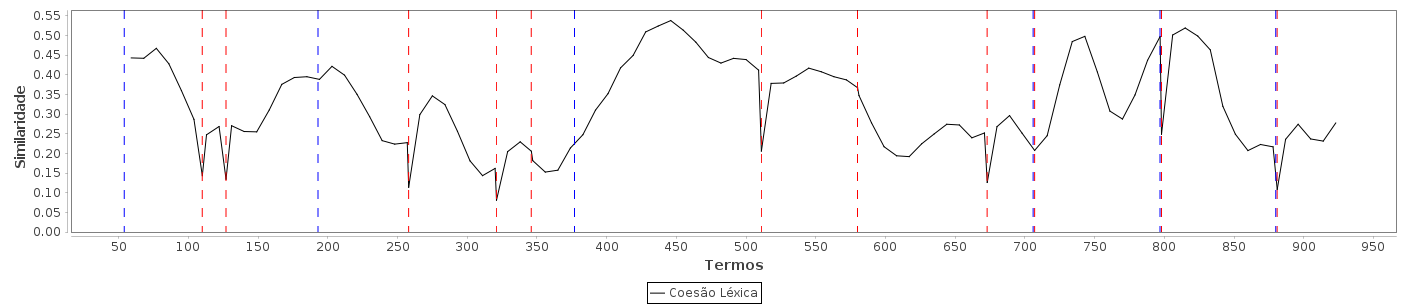
\includegraphics[width=\textwidth]{conteudo/capitulos/figs/coesaolexicaTT-50-9.png}
	  % \caption{Variação da coesão léxica ao longo de uma ata junto a uma segmentação automática em contraste com uma segmentação de referência.}
	  % \label{fig:coesaolexicaTT}
  % \end{figure}




Na Tabela~\ref{tab:resultadosc99} são apresentadas, as médias obtidas com o \textit{C99} bem como as configurações utilizadas, onde \textbf{S} é a proporção de segmentos em relação a quantidade de candidatos, \textbf{M} é o tamanho do quadro utilizado para criar a matriz de \textit{rankings} e \textbf{W} indica se as sentenças são representadas por vetores contendo a frequência dos termos ou um peso que representa sua importância no documento. % como TF*IDF que seria a frequencia do termo no elemento (sentença ou parágrafo) * a frequecia invertida do termo no documento. 
% indica se os segmentos são representados por vetores contendo a frequência ou um peso das palavras.

% \begin{table}[!h]
	% \centering
	% \begin{tabular}{|l||c|c|c|c||c|c|c|c|} \hline

		% & \multicolumn{4}{c||}{Sem Pré-processamento} 
		% & \multicolumn{4}{c|}{Com Pré-processamento}\\			

		% \textbf{Medida} & 
		% \textbf{S} & 
		% \textbf{M} & 
		% \textbf{W} & 
		% \textbf{Média} &
		% \textbf{S} & 
		% \textbf{M} & 
		% \textbf{W} & 
		% \textbf{Média} \\	\hline

		% P$_k$				& 20 & 9 & Sim & 0,134& 20 & 11 & False	& 0,116 \\ \hline  
		% \textit{WindowDiff}	& 60 & 9 & Sim & 0,411& 60 &  9 & Sim 	& 0,390 \\ \hline  
		% Acurácia			& 60 & 9 & Sim & 0,588& 60 &  9 & Sim 	& 0,609 \\ \hline  
		% Precisão			& 40 & 9 & Sim & 0,645& 20 & 11 & False	& 0,720 \\ \hline  
		% Revocação			& 80 & 9 & Sim & 0,869& 80 & 11 & Sim 	& 0,897 \\ \hline  
		% F$^1$				& 80 & 9 & Sim & 0,638& 80 & 11 & Sim 	& 0,655 \\ \hline  

	% \end{tabular}
	% \caption{Resultados obtidos com o \textit{C99}}
	% \label{tab:resultadosc99}
% \end{table}



Verificou-se que, entre os métodos baseados em coesão léxica, o \textit{C99} obteve melhor desempenho em acurácia, precisão, $F^1$, $P_k$ e \textit{WindowDiff}, em relação ao \textit{TextTiling}, enquanto este obteve o melhor desempenho em revocação. De maneira geral, o algoritmo \textit{C99} apresenta melhores resultados em relação ao \textit{TextTiling}, contudo testes estatísticos realizados indicaram que não houve diferença significativa entre os métodos. 



% --> colocar os CDs aqui?

% Com os testes anteriores obteve-se, para cada medida, 4 configurações levando em conta ambos os algoritmos e a presença ou ausência do pré-processamento. Por meio do teste de Friedman e Nemenyi e verificou-se que não há diferença crítica entre os métodos \textit{TextTiling} e \textit{C99}. Na Figura~\ref{fig:CDs} é mostrado os Diagramas para as medidas \textit{WindowDiff}, $P_k$, Acurácia, Precisão, Revocação e $F^1$.	

% \begin{figure}[!h]
	% \centering     %%% not \center

	% \subfigure[a]{ \label{fig:a}
		% 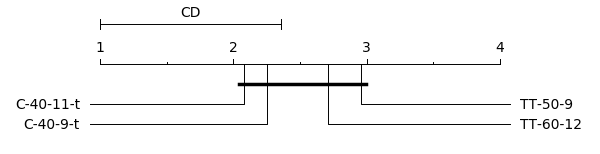
\includegraphics[width=70mm]{conteudo/capitulos/figs/CDs/WinDiff.png} }	
	% \subfigure[b]{ \label{fig:b}
		% 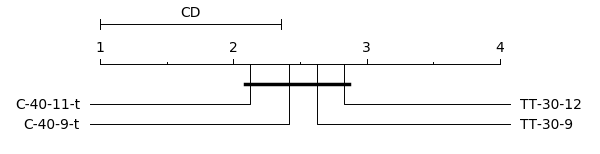
\includegraphics[width=70mm]{conteudo/capitulos/figs/CDs/Pk.png} }
	% \subfigure[c]{ \label{fig:c}
		% 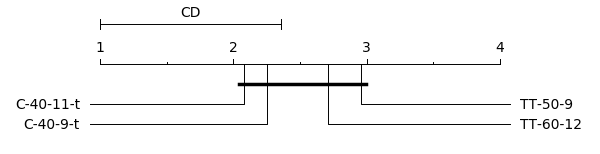
\includegraphics[width=70mm]{conteudo/capitulos/figs/CDs/Acuracy.png}}
	% \subfigure[d]{ \label{fig:d}
		% 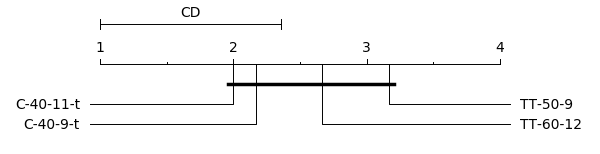
\includegraphics[width=75mm]{conteudo/capitulos/figs/CDs/Precision.png}}
	% \subfigure[e]{ \label{fig:e}
		% 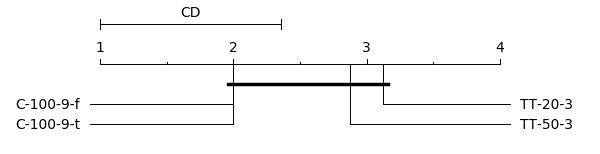
\includegraphics[width=70mm]{conteudo/capitulos/figs/CDs/Recall.png}}
	% \subfigure[f]{ \label{fig:f}
		% 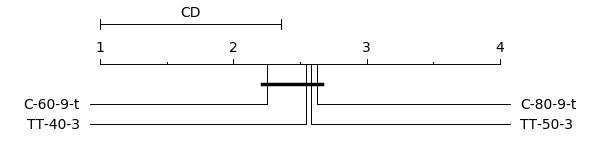
\includegraphics[width=70mm]{conteudo/capitulos/figs/CDs/F1.png}}

		% \caption{Diagramas de Diferença Crítica sobre \textit{ranking} dos algoritmos de segmentação baseados em coesão léxica de acordo com valores de \textit{WindowDiff}, $P_k$, Acurácia, Precisão, Revocação e $F^1$.}
	% \label{fig:CDs}
% \end{figure}
% % -< Colocar uma explicação mais detalhada para esses passos
% % --> Fechar falando sobre os métodos baseados em coesão léxica.




A avaliação final foi feita pela comparação dos resultados dos algoritmos com a segmentação de referência usando as medidas \textit{Pk} e \textit{WindowDiff}. É apresentada também, para fins de comparação com outros trabalhos, as medidas tradicionais acurácia, precisão, revocação e F$^1$, entretanto, nesse contexto, essas medidas são menos significativa que P$_k$ e \textit{WindowDiff}, conforme já mencionado na Seção~\ref{subsec:medidas-segmentacao}. 
Cada técnica foi executada variando seus principais parâmetros a fim de verificar qual configuração melhor otimiza cada algoritmo. A Tabela~\ref{tab:resumo-resultados} contém a média dos dados obtidos onde os melhores resultados estão destacados. Vale lembrar que P$_k$ e \textit{WindowDiff} são medidas de dissimilaridade, ou seja, os valores menores significam melhores resultados.



\begin{table}[!h]
	\centering
	\begin{tabular}{|l||c|c|c|c|c|c|c|c|c|c|c|} \hline

		\textbf{Algoritmo} && 
		\textbf{Step} &
		\textbf{Win} & 
		\textbf{P$_k$} & 
		\textbf{WD} & 
		\textbf{Ac} & 
		\textbf{Pr} & 
		\textbf{Re} &
		\textbf{F$^1$} &
		\textbf{\#Segs} \\	\hline

TextTiling && 20 & 30 & 0.461 & 0.444 & 0.581 & 0.560 & \cellcolor{gray!20} \textbf{0.336} & \cellcolor{gray!20} \textbf{0.411} & 8.833  \\ \hline 
TextTiling && 30 & 45 & \cellcolor{gray!20} \textbf{0.450} & \cellcolor{gray!20} \textbf{0.435} & \cellcolor{gray!20} \textbf{0.596} & \cellcolor{gray!20} \textbf{0.696} & 0.275 & 0.373 & 6.417  \\ \hline 

\hline
		\textbf{Algoritmo} &
		\textbf{RS} &
		\textbf{W} & 
		\textbf{SRate}& 
		\textbf{P$_k$} & 
		\textbf{WD} & 
		\textbf{Ac} & 
		\textbf{Pr} & 
		\textbf{Re} &
		\textbf{F$^1$} &
		\textbf{\#Segs} \\	\hline

C99 & 3 & true  &0.300 &  \cellcolor{gray!20} \textbf{0.434} & \cellcolor{gray!20} \textbf{0.407} & 0.607 & 0.655 & 0.376 & 0.457 & 9.250  \\ \hline 
C99 & 3 & true  &0.700 &  0.485 & 0.431 & 0.602 & 0.553 & \cellcolor{gray!20} \textbf{0.797} & \cellcolor{gray!20} \textbf{0.633} & 21.417  \\ \hline 
C99 & 5 & true  &0.500 &  0.460 & 0.421 & \cellcolor{gray!20} \textbf{0.609} & 0.580 & 0.600 & 0.571 & 15.500  \\ \hline 
C99 & 3 & false &0.200 &  0.448 & 0.427 & 0.596 & \cellcolor{gray!20} \textbf{0.719} & 0.257 & 0.362 & 6.083  \\ \hline 


\hline
		\textbf{Algoritmo} && 
		\textbf{Cut} & 
		\textbf{SRate} &
		\textbf{P$_k$} & 
		\textbf{WD} & 
		\textbf{Ac} & 
		\textbf{Pr} & 
		\textbf{Re} &
		\textbf{F$^1$} &
		\textbf{\#Segs} \\	\hline


MinCutSeg && 13 & 0.300 & 0.457 & 0.427 & 0.594 & \cellcolor{gray!20} \textbf{0.638} & 0.353 & 0.433 & 8.667  \\ \hline 
MinCutSeg && 9  & 0.400 & \cellcolor{gray!20} \textbf{0.444} & 0.408 & \cellcolor{gray!20} \textbf{0.614} & 0.629 & 0.494 & 0.526 & 11.917  \\ \hline 
MinCutSeg && 11 & 0.500 & 0.459 & \cellcolor{gray!20} \textbf{0.407} & 0.603 & 0.588 & 0.590 & 0.563 & 15.000  \\ \hline 
MinCutSeg && 5  & 0.700 & 0.528 & 0.438 & 0.567 & 0.536 & \cellcolor{gray!20} \textbf{0.746} & \cellcolor{gray!20} \textbf{0.599} & 21.000  \\ \hline 


\hline
		\textbf{Algoritmo} &
		\textbf{Prior} &
		\textbf{Disp.} & 
		\textbf{SRate}& 
		\textbf{P$_k$} & 
		\textbf{WD} & 
		\textbf{Ac} & 
		\textbf{Pr} & 
		\textbf{Re} &
		\textbf{F$^1$} &
		\textbf{\#Segs} \\	\hline


 BayesSeg & 0.0800 & 0.5000 &  Auto & \cellcolor{gray!20} \textbf{0.380} & \cellcolor{gray!20} \textbf{0.361} & \cellcolor{gray!20} \textbf{0.655} & 0.662 & 0.479 & 0.551 & 10.000  \\ \hline 
 BayesSeg & 0.1100 & 0.5000 &  Auto & 0.388 & 0.370 & 0.649 & \cellcolor{gray!20} \textbf{0.672} & 0.433 & 0.523 & 9.000  \\ \hline 
 BayesSeg & 0.1100 & 0.1000 & 0.600 & 0.462 & 0.399 & 0.615 & 0.574 & 0.724 & \cellcolor{gray!20} \textbf{0.619} & 18.417  \\ \hline 
 BayesSeg & 0.0800 & 0.1000 & 0.900 & 0.645 & 0.517 & 0.490 & 0.478 & \cellcolor{gray!20} \textbf{0.878} & 0.600 & 27.500  \\ \hline 

\hline
		\textbf{Algoritmo} &&&
		\textbf{SRate} & 
		\textbf{P$_k$} & 
		\textbf{WD} & 
		\textbf{Ac} & 
		\textbf{Pr} & 
		\textbf{Re} &
		\textbf{F$^1$} &
		\textbf{\#Segs} \\	\hline

TextSeg &&& Auto & \cellcolor{gray!20} \textbf{0.455} & 0.439 & 0.585 & \cellcolor{gray!20} \textbf{0.618} & 0.266 & 0.368 & 6.417  \\ \hline 
TextSeg &&& 0.500 & 0.475 & \cellcolor{gray!20} \textbf{0.417} & \cellcolor{gray!20} \textbf{0.594} & 0.565 & 0.608 & 0.566 & 15.500  \\ \hline 
TextSeg &&& 0.900 & 0.604 & 0.484 & 0.524 & 0.498 & \cellcolor{gray!20} \textbf{0.922} & \cellcolor{gray!20} \textbf{0.627} & 27.500  \\ \hline 

\hline
		\textbf{Algoritmo} &&&
		\textbf{SRate} & 
		\textbf{P$_k$} & 
		\textbf{WD} & 
		\textbf{Ac} & 
		\textbf{Pr} & 
		\textbf{Re} &
		\textbf{F$^1$} &
		\textbf{\#Segs} \\	\hline


Sentenças &&& 1.000& \cellcolor{gray!20} \textbf{0.640} & \cellcolor{gray!20} \textbf{0.490} & \cellcolor{gray!20} \textbf{0.506} & \cellcolor{gray!20} \textbf{0.488} & \cellcolor{gray!20} \textbf{1.000} & \cellcolor{gray!20} \textbf{0.638} & 30.500  \\ \hline 



	\end{tabular}
	\caption{Resultados}
	\label{tab:resumo-resultados}
\end{table}





% TODO --> Comentar a tabela 
De maneira geral, as algoritmos avaliados sobressaem ao obtido pela simples atribuição de segmentos a todas sentenças. Observa-se também que os valores de P$_k$ e WD são próximos devido a natureza similar dessas medidas. Pode-se notar também que as configurações que produzem os melhores valores de acurácia também registram melhores valores de P$_k$ ou WD como se vê para \textit{TextTiling}, \textit{MinCutSeg}, \textit{BayesSeg} à exceção de \textit{C99} que registra sua melhor acurácia muito próxima à obtida na configuração ótima para P$_k$ e WD. 
Essa semelhança entre as medidas que toleram proximidade entre segmentações (P$_k$ \textit{WindowDiff}) e a acurácia que apenas computa limites exatos, sugere que quando os anotadores concordam que dois blocos de texto referem-se a assuntos diferentes, também concordam no ponto exato onde há transição de assunto.  Esses resultados são ilustrados graficamente na Figura~\ref{fig:resumo-segmentadores}.
% Todo: Poderia motivar mais pesquisas em Hieraquias de tópicos?
% Todo: E dai? --> Sugere que segmentações ou são idênticas ou não são próximas, ou ainda que quando os anotadores (raramente) concordam, seus limites coincidem examente na maioria dos casos.



Durante os testes analisou-se a influência das parâmetros na eficiência dos algoritmos, em que observou-se que a proporção de segmentos extraídos causam maior impacto nas medidas de desempenho. Na Figura~\ref{fig:influencia-SegRate} é exibida a relação entre a taxa de segmentação e as medidas de desempenho as quais apresentam melhores valores entre $30\%$ e $50\%$ de sentenças marcadas como final de segmento.



\begin{figure}[!h] \centering     %%% not \center

	\subfigure{ \label{fig:influencia-segRate-c99}
	  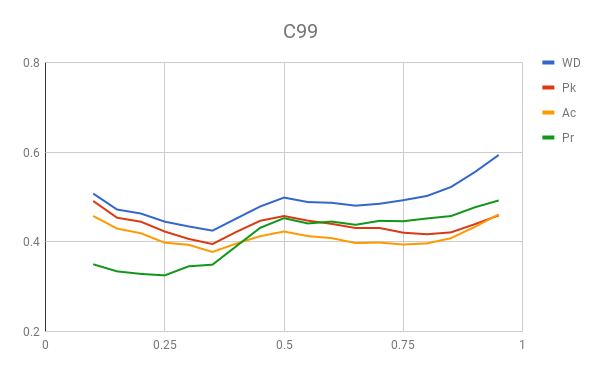
\includegraphics[width=.48\textwidth]{conteudo/capitulos/figs/graficos/analiseNSegRate-C99.png}
	}
	\subfigure{ \label{fig:influencia-segRate-mc}
	  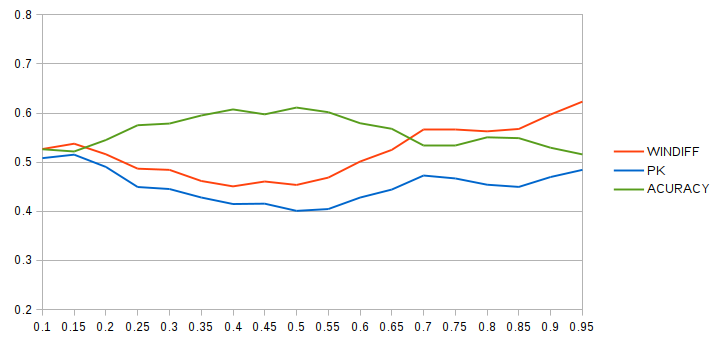
\includegraphics[width=.48\textwidth]{conteudo/capitulos/figs/graficos/analiseNSegRate-MinCut.png}
	}
	\subfigure{ \label{fig:influencia-segRate-bs}
	  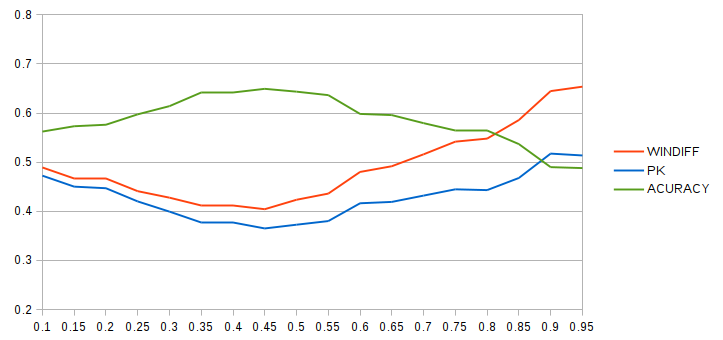
\includegraphics[width=.48\textwidth]{conteudo/capitulos/figs/graficos/analiseNSegRate-Bayes.png}
	}
	\subfigure{ \label{fig:influencia-segRate-ui}
	  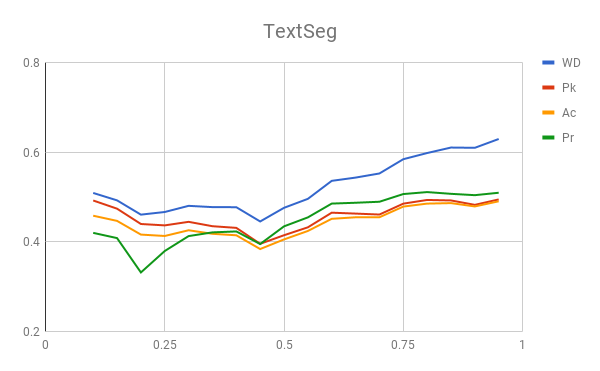
\includegraphics[width=.48\textwidth]{conteudo/capitulos/figs/graficos/analiseNSegRate-UISeg.png}
	}
	\caption{Influência do taxa segmentos na eficiência dos algoritmos}
	\label{fig:influencia-SegRate}
\end{figure}




%%%%%%%%%%%%%%%%%%%%%%
% Análise da Coesão Léxica e eficiência da técnica do TT
%%%%%%%%%%%%%%%%%%%%%%

% --> Falar da coesão léxica peculiar das atas!!

A abordagem baseada em janelas deslisantes empregada no \textit{TextTiling} não permite a configuração direta da quantidade de segmentos extraídos, possibilitando o ajuste do tamanho do passo e comprimento da janela que influenciam seu comportamento nesse aspecto, os quais são analisados a seguir.
Uma vez que a coesão léxica é pressuposto de muitas abordagens em segmentação textual, fez-se uma análise desses documentos quanto a similaridade dos termos ao longo do texto. Verificou-se que a técnica de janelas deslizantes empregada pelo TextTiling encontra os vales que indicam transições entre segmentos, contudo ao comparar esses vales com a segmentação de referência, nota-se que a maioria dos limites coincide ou estão próximos aos vales, porém há casos onde a referência indica limites em trechos com alta coesão léxica e outros onde a queda da coesão, indicada por vales, não coincide com nenhum limite de referência.  

% Na Figura~\ref{fig:coesaolexicaTT}a linha horizontal representa a variação da coesão léxica ao longo de uma ata e as linha verticais azuis e vermelhas representam os limites entre segmentos atribuidos pela referência e pelo algoritmo respectivamente. 
Na Figura~\ref{fig:coesaolexicaTT} é apresentado a variação da coesão léxica ao longo de uma ata e a segmentação obtida pelo \textit{TextTiling} usando tamanho de janela igual a 50 e passo 9. A linha horizontal representa a variação da coesão léxica e as linha verticais azuis e vermelhas representam os limites entre segmentos atribuídos pela referência e pelo algoritmo respectivamente. 


  %--- ---
  \begin{figure}[!h]
	  \centering
	  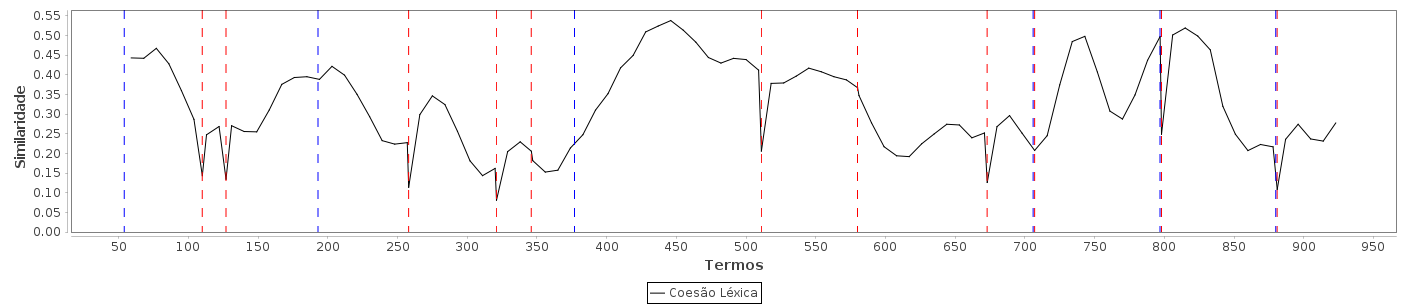
\includegraphics[width=\textwidth]{conteudo/capitulos/figs/coesaolexicaTT-50-9.png}
	  \caption{Variação da coesão léxica ao longo de uma ata junto a uma segmentação automática em contraste com uma segmentação de referência.}
	  \label{fig:coesaolexicaTT}
  \end{figure}









Em termos de performance, o modelo implementado no algoritmo \textit{BayesSeg} apresenta melhores para as medidas P$_k$ e \textit{WindowDiff}, visto que essas são mais adequadas ao contexto analisado, este será empregado nos próximos experimentos. Contudo, dado a subjetividade da tarefa de segmentação textual, outros modelos podem ser utilizados satisfatoriamente dependendo do critério adotado. 


\begin{figure}[!h] \centering     %%% not \center

	\subfigure{ \label{fig:resumo-wd-pk}
		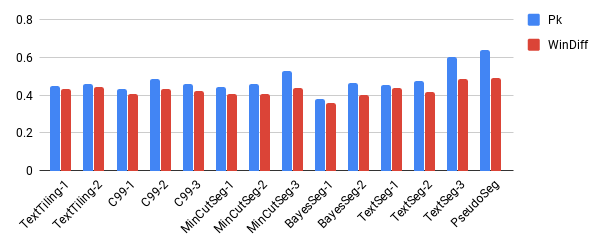
\includegraphics[width=.49\textwidth]{conteudo/capitulos/figs/graficos/resumo-wd-pk.png}	
	\subfigure{ \label{fig:resumo-tradicionais}
		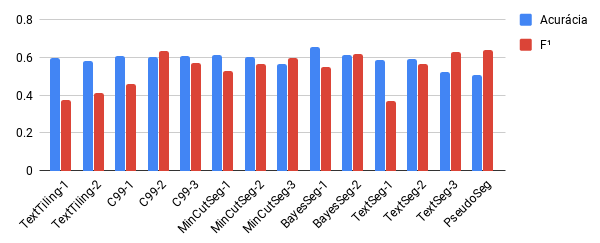
\includegraphics[width=.49\textwidth]{conteudo/capitulos/figs/graficos/resumo-tradicionais.png}	
	}
	\caption{Performance dos algoritmos de segmentação textual}
	\label{fig:resumo-segmentadores}
\end{figure}



% TODO --> Comentar as WD e PK

Na Figura~\ref{fig:resumo-tradicionais} é apresentada a performance dos algoritmos nas medidas tradicionais. Observa-se valores altos de revocação para a segmentação por sentenças, pois é atribuído um limite a todo candidato a final de segmento, o que resulta no valor máximo para revocação. De maneira semelhante, o comportamento do \textit{TextTiling} gera menos segmentos em relação aos demais, e com isso tem-se valores menores de revocação, o que pode ser alterado pela configuração do algoritmo com passos mais curtos, ou ainda, sobre-escrevendo a função que calcula os \textit{depth scores} para reconhecer vales menos profundos.



% De maneira geral, os métodos probabilísticos apresentam desempenho próximo 



Após a análise dos métodos, selecionou-se o algoritmo que apresenta melhores resultados para as medidas P$_k$ e \textit{WindowDiff} visto a subjetividade da tarefa e a aderência dessas medias à acurácia e precisão. Realizou-se então uma experimento a fim de avaliar subjetivamente o segmentador escolhido em conjunto com extratores de tópicos e analisar essas técnicas.




  % Após a identificação dos segmentos, o algoritmo retorna uma lista com fragmentos do texto original. Cada segmento é incorporado à estrutura de dados interna como subdocumentos com um tema relativamente independente. Em seguida, esses subdocumentos serão analisados pelo extrator de tópicos para identificação de descritores e agrupamento.







\chapter{Avaliação dos Extratores de Tópicos}\label{cap-extratores}

% Dar uma geral nesse primeiro parágrafo
	% Escolha dos Algorítmos
	% Escolha do método de avaliação (subjetivo com questionario)

% -- 1 - Motivação para o experimento.
Nesse capítulo, as técnicas de extração de tópicos são analisadas. O objetivo é comparar os algoritmos de extração de tópicos na tarefa de extração de padrões no contexto das atas de reunião no que tange a qualidade dos agrupamentos e seus descritores bem como sua capacidade de representar os segmentos. Escolheu-se os modelos LDA, PLSA e K-Means para essa análise devido a popularidade desses métodos os quais são amplamente utilizados~\cite{DZhu20122} e frequentemente referenciados em trabalhos voltados a organização de bases textuais~\cite{Aggarwal2018, OCallaghan2015, Steyvers2007}.
Os algoritmos foram inicialmente configurados com base em avaliações internas~\cite{Hassani2017} e observações empíricas nas quais escolheu-se os melhores valores para seus parâmetros. Os resultados desses modelos foram submetidos a uma avaliação subjetiva a fim de analisá-los junto a usuários com afinidade com atas de reuniões. 

Nessa avaliação, a técnica de segmentação textual também foi avaliada, uma vez que é a etapa anterior a extração de tópicos está diretamente ligada a os resultados apresentados ao avaliador bem como pode interferir no funcionamento dos modelos de extração de tópicos. Assim, a técnica de segmentação textual foi avaliada subjetivamente em complemento a análise estatística apresentada no Capítulo~\ref{cap-segmentadores}.

A avaliação se deu por meio de questionários onde profissionais com afinidade com atas de reunião forneceram suas percepções em relação aos resultados dos modelos de extração de tópicos. Por fim, os dados obtidos dos experimentos serviram de base para as análises dos algoritmos e de sua aplicação no contexto das atas de reuniões.
% os dados serviram como base para análise dos algoritmos 

\section{Configuração experimental}

% A qtd de tópicos é um parametro importante.  % Todos com 70 tópicos e 5 extratores;
Durante os primeiros testes empíricos a qualidade dos resultados mostrou-se sensível à quantidade de tópicos extraídos.
Inicialmente, realizou-se um teste prévio utilizando uma versão não-paramétrica dos algorítimos a fim de automaticamente obter valores ótimos para esse parâmetro por meio da análise das medidas Silhueta e Coesão. Essa configuração automática resulta valores em torno de 20 tópicos. Contudo, apresenta grupos com muitos segmentos (em torno de 100) o que os tornam pouco coesos além de certa dificuldade em julgar capacidade dos descritores em representar bem o tópico.  
Em observações diretas, valores próximos a entre 60 e 80 mostraram melhores resultados. Nesse trabalho, optou-se por configurar os algoritmos para extrair 70 tópicos da coleção de segmentos por apresentar melhores resultados aparentes na visão de usuário.

Outro fator importante é a quantidade de descritores selecionados para cada tópico. Com base no experimento de anotações em segmentação, descrito no Capítulo~\ref{cap2}, os anotadores selecionaram em média 5 palavras para descrever os segmentos, sendo esse valor adotado para essa avaliação.




\section{Critérios de avaliação}


% - Explicar que foram 2 consultas (quais) e mostrar os extratores.
% - 4 - Procedimento (2 consultas, técnicas em ordens diferentes).
Após a configuração, cada um dos modelos de extração de tópicos foi submetido a duas consultas: ``\textit{compra de equipamentos}'' e ``\textit{defesa de dissertação}'' gerando 6 cenários distintos a serem analisados. 
Para cada cenário, o sistema seleciona o tópico com maior relevância com a consulta e em seguida exibe 5 segmentos desse tópico escolhidos aleatoriamente. 
Vale dizer que nessa avaliação as técnicas de ranqueamento dos resultados não são aplicadas para que estas não interfiram na avaliação dos extratores, contudo, o sistema final poderá ranquear também os segmentos com maior relevância de um ou mais tópicos por meio de técnicas de recuperação de informação. 
Os resultados desses cenários foram apresentados a um grupo de avaliadores que individualmente avaliaram a qualidade das técnicas de extração de tópicos. 
%

% -- 3 - Escolha dos participantes.
O perfil dos avaliadores é de profissionais da area acadêmica/escolar devido à sua afinidade com o ambiente de gestão e conhecimentos de assuntos relacionados ao \textit{corpus} estudado nesse trabalho. O grupo convidado a participar do experimento é formado por 24 profissionais da UFSCar campus Sorocaba, 13 profissionais de escolas técnicas e 3 profissionais de escolas do Ensino Fundamental, sendo 11 ocupantes de cargos de gestão como coordenadores de curso, diretores, 17 membros de conselhos, 5 profissionais administrativos e 3 professores, totalizando 40 avaliadores em que a maioria afirma ter afinidade com atas e reuniões e 3 declararam nenhuma afinidade com esses documentos. Os avaliadores foram divididos em dois grupos onde cada grupo avaliou as técnicas de extração tópicos a partir de uma consulta (palavras-chave), ou seja, cada indivíduo avaliou 3 cenários distintos. A avaliação consistiu de um documento impresso contendo uma breve apresentação do trabalho, seguido de uma cópia dos resultados das técnicas de extração de tópicos e questões avaliativas sobre cada técnica.

% X profissionais de gestão de instituições 

% -- 2 - Escolha das questões.
O questionário foi formado por questões envolvendo aspectos os extratores de tópicos e questões referentes à técnica de segmentação textual empregada
As respostas seguiram a escala \textit{Likert}~\cite{Norman2010} com 5 alternativas. 
% , conforme mostrado:

\begin{enumerate}
	\item Todos os trechos apresentados compartilham um mesmo assunto.
	\item As palavas \textit{<descritores>} resumem bem o assunto tratado nos trechos.
	\item Existem trechos que não tratam de um único assunto?
	\item Existem trechos incompletos e insuficientes para compreensão do assunto do trecho?
\end{enumerate}


As questões 1 e 2 estão relacionadas ao extrator de tópicos. A primeira refere-se ao agrupamento dos segmentos pela qual foi avaliada a semelhança dos trechos em termos de assunto. A segunda questão diz respeito aos descritores selecionados, ao respondê-la o avaliador indicou o quão bem esses termos representam aquele grupo.
As questões 3 e 4 estão ligadas à técnica de segmentação utilizada, o BayesSeg conforme já mencionado no Capítulo~\ref{cap-segmentadores}. A questão 3 está ligada à coesão de cada segmento, levando em conta a homogeneidade do texto em relação a um assunto. A questão 4 refere-se a completude dos segmentos, ou seja, o quão bem os segmentos podem ser bem compreendidos independentemente da leitura do documento integral.
Para afastar a hipótese de que os resultados das técnicas fossem influenciados pela ordem apresentada, essas foram apresentadas aos avaliadores em ordem aleatórias.
% -- 5 - Escolha dos temas para consulta: 




% A primeira refere-se ao agrupamento dos segmentos pela qual foi avaliada a semelhança dos trechos em termos de assunto.

\section{Resultados}

Nessa seção, os dados coletados das avaliações são apresentados e analisados. Os modelos de extração de tópicos discutidos nesse trabalhos são comparados de acordo com os critérios mencionados anteriormente: 
(1) comparar algoritmos de extração de tópicos na tarefa de extração de padrões no contexto das atas de reunião, 
(2) analisar a qualidade dos agrupamentos no que tange a navegação por grupos com mesmo tópico, 
(3) analisar a qualidade dos descritores extraídos para recuperar os documentos dos grupos,
(4) validar a performance do segmentador empregado.


Na Figura~\ref{fig:Q1} é apresentado as frequência das respostas coletadas sobre a primeira questão a qual refere-se a qualidade do agrupamento levando em conta a semelhança dos segmentos em termos de assunto. Verifica-se que o K-Means tem resultados similares ao LDA enquanto o PLSA se mostrou menos eficiente nesse critério uma vez que mais avaliadores rejeitaram a afirmação de que todos os segmentos tratam de um único assunto em comum. 

\begin{figure}[!h] \centering     %%% not \center

	\subfigure{ \label{fig:kmeans}
		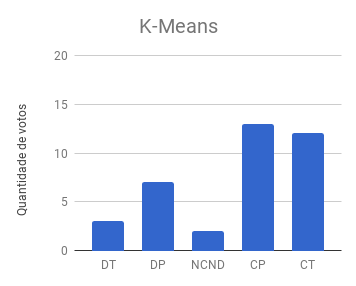
\includegraphics[width=.31\textwidth]{conteudo/capitulos/figs/figuras-experimento/Q1-KMeans.png}
	}	
	\subfigure{ \label{fig:lda}
		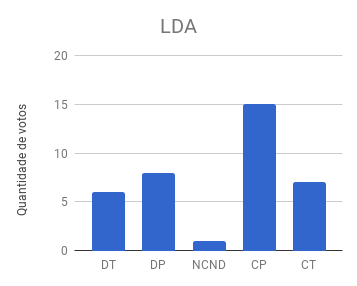
\includegraphics[width=.31\textwidth]{conteudo/capitulos/figs/figuras-experimento/Q1-LDA.png}
	}
	\subfigure{ \label{fig:plsa}
		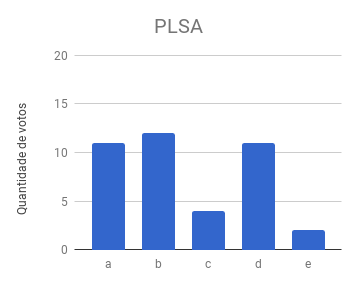
\includegraphics[width=.31\textwidth]{conteudo/capitulos/figs/figuras-experimento/Q1-PLSA.png}
	} 
	\caption{Contagem de respostas referente a primeira questão cujo enunciado foi:\textit{``Todos os trechos apresentados compartilham um mesmo assunto.''}. O eixo vertical indica a frequência das alternativas representadas no eixo horizontal por:
		a=\textit{``Discordo Totalmente''}
		b=\textit{``Discordo Parcialmente''}
		c=\textit{``Não Concordo, nem Discordo''}
		d=\textit{``Concordo Parcialmente''}
		e=\textit{``Concordo Totalmente''}.
	}
	\label{fig:Q1}
\end{figure}



% A segunda questão diz respeito aos descritores selecionados, ao respondê-la o avaliador indicou o quão bem esses termos representam aquele grupo.
Outro ponto importante a ser analisado é a capacidade representativa dos descritores, ou seja, o quão bem os descritores podem representar o tópico ao qual os segmentos foram atribuídos. Observa-se na Figura~\ref{fig:Q2} no K-Means a maior diferença entre as opiniões positivas e negativas, sendo a maioria concordante com a afirmação de que os descritores extraídos são bons atributos para descrever o teor dos segmentos extraídos.

\begin{figure}[!h] \centering     %%% not \center

	\subfigure{ \label{fig:kmeans}
		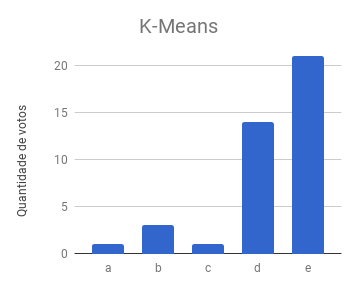
\includegraphics[width=.31\textwidth]{conteudo/capitulos/figs/figuras-experimento/Q2-KMeans.png}
	}	
	\subfigure{ \label{fig:lda}
		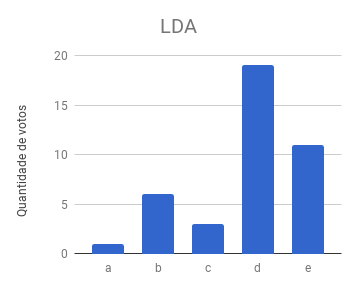
\includegraphics[width=.31\textwidth]{conteudo/capitulos/figs/figuras-experimento/Q2-LDA.png}
	}
	\subfigure{ \label{fig:plsa}
		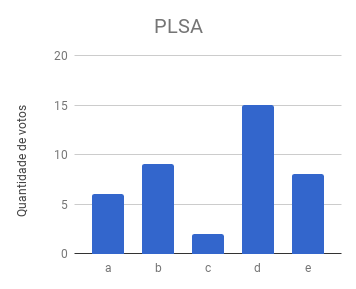
\includegraphics[width=.31\textwidth]{conteudo/capitulos/figs/figuras-experimento/Q2-PLSA.png}
	}
	\caption{Contagem de respostas referente a segunda questão cujo enunciado foi:\textit{``As palavas <descritores> resumem bem o assunto tratado nos trechos.''}. O eixo vertical indica a frequência das alternativas representadas no eixo horizontal por:
		a=\textit{``Discordo Totalmente''}
		b=\textit{``Discordo Parcialmente''}
		c=\textit{``Não Concordo, nem Discordo''}
		d=\textit{``Concordo Parcialmente''}
		e=\textit{``Concordo Totalmente''}.
	}
	\label{fig:Q2}
\end{figure}


% -- Conclusão : extração de padrões	
Ao analisar os resultados, verifica-se que de maneira geral os modelos K-Means e LDA podem ser considerados satisfatórios na tarefa de agrupar e representar os segmentos das atas.
Verifica-se também que para o modelo K-Means os avaliadores identificaram que, na maioria dos casos, houve resultados satisfatórios, principalmente quanto a representatividade dos descritores. Embora a avaliação aponte imperfeições, esse modelo apresenta maior uniformidade em relação aos demais.


Esse experimento foi aproveitado para validar o segmentador empregado nesse trabalho. Uma vez que esta uma etapa anterior à extração de tópicos a princípio, a modelo que selecionou os segmentos não interfere em sua avaliação. Assim, a Figura~\ref{fig:Q3e4} mostra as respostas do avaliadores considerando todos os cenários. As respostas referentes a terceira questão, na qual se averígua a homogeneidade de cada segmento quanto ao seu assunto central, apontam que poucos segmentos contém mais de um assunto.
Ainda sobre a qualidade da segmentação, a quarta questão investiga a integridade de cada segmento, isto é, sua capacidade de informar o usuário sobre o assunto que trata sem necessidade de se recorrer a leitura do documento integral. Nesse critério, a maioria das avaliações indicam que nenhum ou poucos segmentos apresentam texto insuficiente para leitura.  Uma análise mais detalhada das questões relacionadas a segmentação das atas foi discutida no Capítulo~\ref{cap-segmentadores}, ficando aqui análises de pontos onde a segmentação influencia os extratores e os resultados finais apresentados ao usuário.


\begin{figure}[!h] \centering     %%% not \center

	\subfigure{ \label{fig:seg1}
		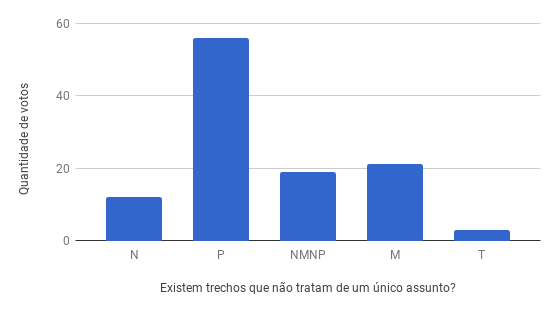
\includegraphics[width=.48\textwidth]{conteudo/capitulos/figs/figuras-experimento/Q3-Seg.png}
	}	
	\subfigure{ \label{fig:seg2}
		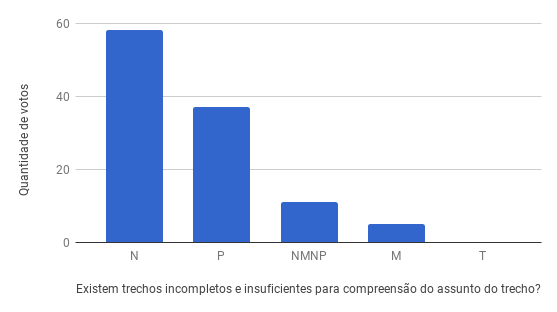
\includegraphics[width=.48\textwidth]{conteudo/capitulos/figs/figuras-experimento/Q4-Seg.png}
	}
	\caption{Contagem de respostas referente a terceira e quarta questão. Os eixos verticais indicam as frequências das alternativas representadas no eixos horizontais por:
		a=\textit{``Nenhum''}
		b=\textit{``Poucos''}
		c=\textit{``Nem Muitos, nem Poucos''}
		d=\textit{``Muitos''}
		e=\textit{``Todos''}.
	}
	\label{fig:Q3e4}
\end{figure}


Outra questão analisada foi o comportamento dos modelos nas diferentes consultas. Ao se isolar as respostas das questões referentes a uma consulta específica, nota-se certa alteração nas respostas dos modelos. 
Os gráficos apresentados na Figura~\ref{fig:c12-q1}, mostram na primeira superior as respostas para cada modelo considerando-se os segmentos extraídos na primeira consulta e na linha inferior aqueles referentes a segunda consulta. O K-Means apresenta uma diminuição considerável na segunda consulta em relação a primeira no que se refere a respostas afirmando que os todos os segmentos compartilham um único assunto, e um aumento de respostam indicando discordância total com a afirmação da questão.
De forma semelhante, o PLSA apresenta diminuição de respostas positivas para essa afirmação e na proporção que há um aumento de respostas negativas. 
Por outro lado o LDA mantém resultados semelhantes em ambas as consultas, nas quais apresenta resultados equilibrados entre respostas positivas e negativas. Em outras palavras, os modelos K-Means e PLSA sofreram perda de desempenho enquanto o LDA manteve-se estável em ambas consultas.
Ao analisar separadamente a segunda questão, referente a representatividade dos descritores observa-se na Figura~\ref{fig:c12-q2} que todos os modelos apresentam perca de performance nesse critério, contudo, de forma acentuada no PLSA. 



% indicam que o Algoritmo 





\begin{figure}[!h] \centering     %%% not \center

	\subfigure{ \label{fig:c1q1kmeans}
		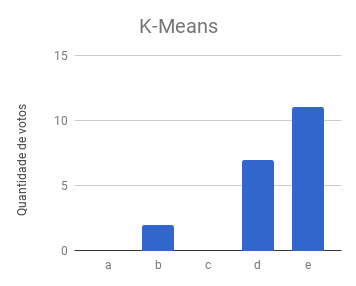
\includegraphics[width=.31\textwidth]{conteudo/capitulos/figs/figuras-experimento/C1-Q1-KMeans.png}
	}	
	\subfigure{ \label{fig:c1q1lda}
		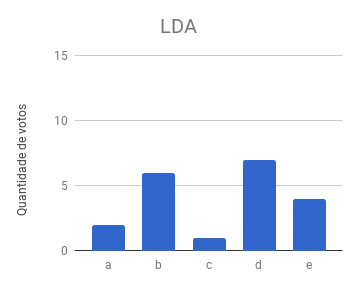
\includegraphics[width=.31\textwidth]{conteudo/capitulos/figs/figuras-experimento/C1-Q1-LDA.png}
	}
	\subfigure{ \label{fig:c1q1plsa}
		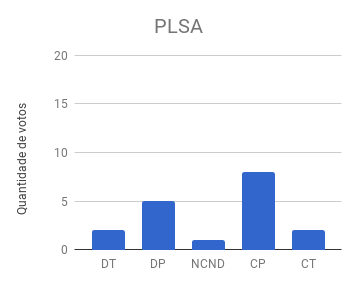
\includegraphics[width=.31\textwidth]{conteudo/capitulos/figs/figuras-experimento/C1-Q1-PLSA.png}
	}
	\subfigure{ \label{fig:c2q1kmeans}
		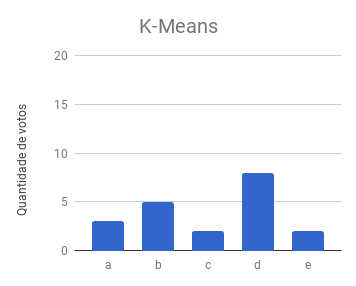
\includegraphics[width=.31\textwidth]{conteudo/capitulos/figs/figuras-experimento/C2-Q1-KMeans.png}
	}	
	\subfigure{ \label{fig:c2q1lda}
		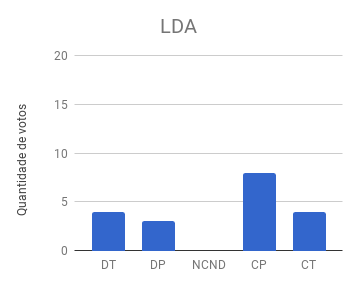
\includegraphics[width=.31\textwidth]{conteudo/capitulos/figs/figuras-experimento/C2-Q1-LDA.png}
	}
	\subfigure{ \label{fig:c2q1plsa}
		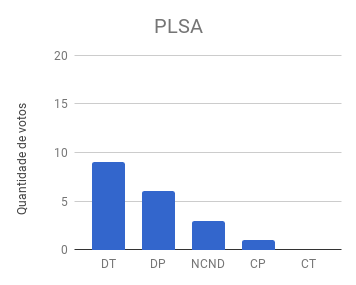
\includegraphics[width=.31\textwidth]{conteudo/capitulos/figs/figuras-experimento/C2-Q1-PLSA.png}
	}

	\caption{Contagem das respostas referentes a Primeira questão. A primeira consulta, ``\textit{compra de equipamentos}'', é mostrada na linha superior e a segunda consulta, ``\textit{defesa de dissertação}'', na linha inferior.}
	\label{fig:c12-q1}
\end{figure}






\begin{figure}[!h] \centering     %%% not \center

	\subfigure{ \label{fig:c1q2kmeans}
		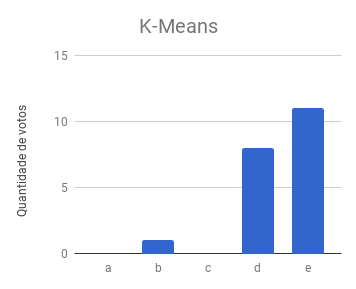
\includegraphics[width=.31\textwidth]{conteudo/capitulos/figs/figuras-experimento/C1-Q2-KMeans.png}
	}	
	\subfigure{ \label{fig:c1q2lda}
		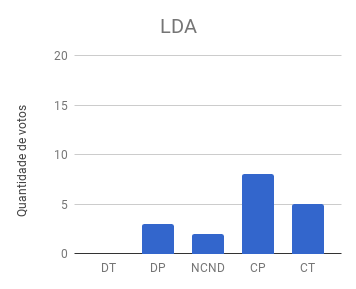
\includegraphics[width=.31\textwidth]{conteudo/capitulos/figs/figuras-experimento/C1-Q2-LDA.png}
	}
	\subfigure{ \label{fig:c1q2plsa}
		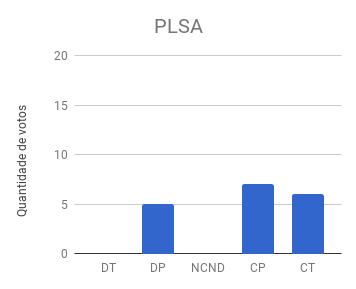
\includegraphics[width=.31\textwidth]{conteudo/capitulos/figs/figuras-experimento/C1-Q2-PLSA.png}
	}
	\subfigure{ \label{fig:c2q2kmeans}
		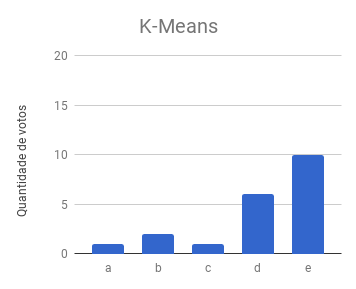
\includegraphics[width=.31\textwidth]{conteudo/capitulos/figs/figuras-experimento/C2-Q2-KMeans.png}
	}	
	\subfigure{ \label{fig:c2q2lda}
		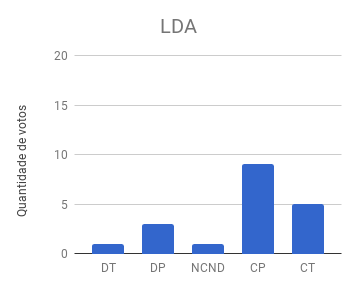
\includegraphics[width=.31\textwidth]{conteudo/capitulos/figs/figuras-experimento/C2-Q2-LDA.png}
	}
	\subfigure{ \label{fig:c2q2plsa}
		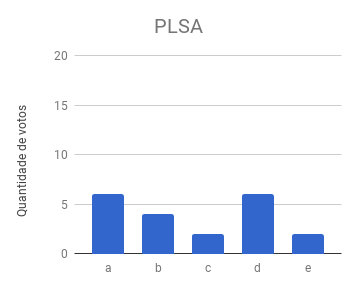
\includegraphics[width=.31\textwidth]{conteudo/capitulos/figs/figuras-experimento/C2-Q2-PLSA.png}
	}

	\caption{Contagem das respostas referentes a Segunda questão. A primeira consulta, ``\textit{compra de equipamentos}'', é mostrada na linha superior e a segunda consulta, ``\textit{defesa de dissertação}'', na linha inferior.}
	\label{fig:c12-q2}
\end{figure}



{
\small
TODO:
--> O segmentador, sendo uma etapa anterior a extração de tópicos, influencia na qualidade do grupos??

--> O K-means traz melhores segmentos (Sem misturar assuntos) em relação aos outros métodos.  'Aparentemente o K-means seleciona os trechos mais coesos, mas precisa de mais experimentos, mais amostras ...'


--> Com os avaliadores das ETECs T1 > T2 > T3
--> Incluindo os da UFSCar   T1 > T2 = T3;
}




% -- Conclusão : do conjunto das técnicas de extração e segmentação

Nessa Seção, analisou-se as técnicas de segmentação textual e extração de tópicos na criação de uma estrutura derivada do \textit{corpus} original como uma representação estruturada da coleção de atas a qual foi organizada e acrescida de atributos para sua descrição. As análises sugerem que tais técnicas podem oferecer a sistemas de recuperação uma representação estruturada que preserva o conteúdo dos documentos ao mesmo tempo que cria atributos adicionais que incorporam informação à base de dados e podem ser inseridas no espaço de busca.  

% Na maioria dos casos, os dados coletados apontam 






% \chapter{Avaliação do Módulo de Consulta}






% \chapter*[Conclusão]{Conclusão}
\chapter{Conclusão}
\label{cap:conclusao}
% \addcontentsline{toc}{chapter}{Conclusão}



% -------------------- Introdução -------------------- 

% Em um contexto em que a grande parte das informações armazenadas pelas organizações está em formato textual, o desenvolvimento de ferramentas computacionais para extração e organização automática dessas informações é uma tarefa que retem atenção e relevância.

Com a grande disponibilidade de dados em formato textual, há um constante interesse no desenvolvimento de ferramentas computacionais para recuperação automática de informações úteis a partir desses dados. 
Dentre os textos usados para registros, identificou-se documentos multi-temáticos, os quais abordam assuntos diversos no mesmo texto, como exemplo, as atas de reuniões apresentam com característica a ausência de meta informações ou mesmo quebras de parágrafos que ajudariam a separar e identificar seus conteúdos. 
Entre as abordagens aplicáveis a este problema estão a segmentação textual e os modelos de extração de tópicos as quais em conjunto são capazes de separar, identificar e agrupar os assuntos contidos nessa categoria de documentos.






% -------------------- Retomada do que foi feito -------------------- 

Sendo assim, este trabalho de mestrado visou o desenvolvimento de um Sistema de Recuperação de Informação utilizando técnicas de Segmentação Textual e Extração de Tópicos para extração automática de conhecimento em uma base de dados composta por atas de reunião coletadas da Universidade Federal de São Carlos, campus Sorocaba. 
Desenvolveu-se uma metodologia que utiliza a segmentação textual para fragmentar as atas em porções de texto com um assunto relativamente independente os quais são agrupados e descritos semanticamente por um modelo de extração de tópicos, conforme apresentado no Capítulo~\ref{cap3}.

Inicialmente, a fim de analisar as técnicas utilizadas, gerou-se um \textit{corpus} anotado por 9 profissionais com afinidade com o domínio investigado. Os anotadores segmentaram e rotularam manualmente 12 atas de reunião. 
Para isso desenvolveu-se uma ferramenta para anotação manual de documentos, pela qual os anotadores forneceram segmentações e informações sobre os segmentos identificados.
Os textos originais acrescidos das informações fornecidas pelos anotadores foram reunidas para formar um \textit{corpus} derivado que ajuda a entender o corpus investigado em termos de sua distribuição de tópicos. Os dados referentes a segmentação manual foram utilizados para criar uma segmentação de referência para avaliação objetiva dos segmentadores. 

A avaliação dos segmentadores considerou os algoritmos e seus principais parâmetros para encontrar o modelo que melhor otimiza a tarefa de segmentação do corpus investigado. Comparou-se os resultados obtidos com a segmentação de referência e verificou-se que o algoritmo \textit{BayesSeg} apresenta resultados melhores em relação às demais técnicas analisadas. Além disso, a escolha escolheu-se o \textit{BayesSeg} devido ao sua abordagem probabilísticas similar a modelos de extração de tópicos como o LDA. 
Os resultados mostram certa dificuldade devido as características das atas, como estilo de escrita e segmentos relativamente curtos, além da subjetividade intrínseca da tarefa.
Embora os métodos de segmentação textual tenham se mostrado suficientes, melhores resultados podem ser alcançados com o acréscimo das técnicas mencionadas e a construção de uma segmentação de referência mais robusta em termos concordância entre os anotadores que ajudaram a criá-la.
Uma vez escolhido o segmentador, este foi utilizado para segmentar os textos de um conjunto de 175 atas, que gerou um conjunto de 1276 segmentos, os quais foram submetidos aos modelos de extração de tópicos.
Detalhes sobre o \textit{corpus} anotado e avaliação objetiva dos segmentadores foram analisados no Capítulo~\ref{cap-segmentadores}.



% -- Estrutura de Dados Interna

Após a avaliação dos segmentadores e segmentação do \textit{corpus} inicial, o desenvolvimento prosseguiu com a avaliação dos extratores de tópicos. Os extratores foram executados para agrupar e extrair descritores do conjunto de segmentos. Cada extrator formou 70 grupos (tópicos) e para cada grupo extraiu 5 descritores. 

A metodologia utilizada nesse trabalho conecta as técnicas de segmentação textual aos modelos de extração de tópicos a fim de gerar um estrutura derivada a partir de um \textit{corpus} não estruturado. Essa nova estrutura concentra os textos originais acrescidos de informação latentes e organizados por sua semelhança semântica. Essa organização permite que técnicas de recuperação de informação expandam o espaço de busca além do conjunto de termos original de cada segmento, sendo assim, favorecidas quanto a identificação segmentos relacionados a consulta do usuário bem como permite a exploração dos grupos com assuntos relacionados.





% -- Avaliação Subjetiva


Os modelos de extração de tópicos foram avaliados subjetivamente por meio de questionários em que 41 avaliadores responderam à questões referentes à qualidade dos trechos apresentados como resultado à consultas à base de dados criada com essa metodologia. 
A fim de avaliar 3 dos principais modelos de extração de tópicos e o segmentador escolhido (\textit{BayesSeg}), o sistema foi submetido a duas consultas distintas, gerando 6 cenários a serem avaliados. 
Os questionários foram formulados para obter primeiramente a percepção dos avaliadores quanto a qualidade dos tópicos extraídos, levando em conta a similaridade dos segmentos em relação ao mesmo assunto e a representatividade dos descritores. 
Os avaliadores também responderam questões referentes a qualidade dos segmentos apresentados, uma vez que a segmentação, embora etapa anterior, é parte do processo de obtenção de conhecimento. Sobre a segmentação, considerou-se a completude dos segmentos a sua unidade em relação ao assunto.
Os dados dos questionários após coletados e analisados, sugerem que a metodologia empregada é capaz de entregar ao usuário resultados satisfatórios. Verificou-se também que o K-Means traz melhores resultados em relação aos demais extratores avaliados. 
A análise detalhada dessas avaliações e a relação entre as técnicas empregadas nessa metodologia foram apresentadas no Capítulo~\ref{cap-extratores}.
% Após coletados e analisados, os dados dos questionários



% -------------------- Contribuições -------------------- 


De modo geral, os resultados obtidos com a utilização das informações extraídas pela metodologia apresentada nesse trabalho recebe uma base de dados constituída por documentos multi-temáticos não estruturada e produz uma estrutura de dados interna mais organizada e acrescida de informações latentes extraídas do próprio \textit{corpus} original de forma não supervisionada. 
A utilização de descritores para expandir a o espaço de busca pelas técnicas de recuperação de informação possibilita ganho em relação a busca indexada por termos presentes nos documentos. Além disso, o retorno procura exibir apenas os trechos relevantes à consulta do usuário, ao invés de documentos inteiros que podem conter trechos irrelevantes à consulta.  
A estrutura dada ao corpus original permite analisar seu conteúdo pela perspectiva da distribuição dos tópicos. Com isso, é possível entender a composição e recorrência dos assuntos discutidos bem como traçar um histórico dos assuntos abordados a fim de visualizar sua evolução ao longo do tempo.


\section{Contribuições}	



Considera-se como principais contribuições deste trabalho o método apresentado para extração de conhecimento em documentos multi-temáticos, o corpus de atas anotadas, o sistema proposto e sua implementação, as avaliações dos segmentadores e dos extratores de tópicos e os resultados produzidos durante a execução da proposta desse sistema. 

A metodologia proposta permite organizar e adicionar informação a coleção de documentos multi-temáticos, com a finalidade de extrair automaticamente conhecimento em atas de reunião. Essa metodologia, pode ainda ser  aproveitada para trazer avanços em estudos e aplicações voltadas à extração e recuperação de informação em outros domínios com as mesmas características. 

O \textit{corpus} anotado produzido contém dados adicionados aos documentos originais os quais ajudam a entender o a distribuição dos tópicos ao longo das atas. O corpus anotado está disponível para servir como base de dados para outros trabalhos, bem como a ferramenta desenvolvida para esse propósito, a qual pode ser utilizada em qualquer \textit{corpus} a ser anotado com fins de pesquisa, bem como modificada livremente. 

O Sistema Proposto e sua implementação podem ser utilizados para extração de conhecimento em bases de dados formadas por documentos multi-temáticos, em especial, conjuntos de atas de reunião. Outras domínios que lidam com bases de dados com as mesmas características podem aproveitar esse sistema bem como seu código fonte para eventuais adaptações ou expansões.
 
As avaliações dos segmentadores mostraram dados objetivos sobre o desempenho dessas técnicas quando aplicadas à coleção de documentos utilizada nesse trabalho. 
A avaliação dos extratores apresentou a percepção de profissionais com afinidade com o contexto das atas de reunião sobre os resultados da combinação entre o segmentador empregado e os extratores de tópicos.






% -------------------- Trabalhos Futuros -------------------- 

\section{Trabalhos Futuros}	

Entre as continuações e futuras melhorias para este trabalho, pode-se citar implementações no próprio sistema proposto e ampliação das bases de dados bem como inclusão de novos \textit{corpora}.  
%
Os primeiros experimentos desse trabalho geraram um artigo que foi submetido para publicação, porém, não foi aceito. Essa recusa exigiu novos experimentos com mais dados os quais são apresentados nessa dissertação. Assim, um novo artigo será submetido em complemento à esse trabalho.
% 
A proposta inicial desse trabalho contempla a classificação dos segmentos em relação ao tipo de menção ao assunto, como decisão, orientação e irrelevante. Os dados colhidos no experimento mencionado na Seção~\ref{sec:anotacoes} referentes ao tipo de menção e contexto do assunto serão utilizados para o gerar um classificador para categorizar automaticamente um segmento nas categorias. Para isso, as anotações coletadas podem ser utilizadas na etapa de treinamento dos classificadores.
%
Outras melhorias do sistema podem ser alcançadas com testes voltados a experiência do usuário a fim de medir a satisfação dos resultados apresentados e guiar a implementação de uma interface gráfica para possibilitar ao usuário analisar os dados pela exploração interativa dos grupos.
%

Cita-se também a utilização de fontes externas para melhorar os métodos de segmentação textual. Recursos como \textit{thesaurus} (dicionários de sinônimos) e \textit{clue words} (palavras-pista) podem adicionar conhecimento externo ao sistema e com isso alcançar melhores resultados. 
%
Pretende-se ainda replicar os experimentos deste trabalho em novas bases de dados com características semelhantes às ata de reunião. Por exemplo, transcrições de conversas, diálogos em \textit{chats,} discursos e atas de outras organizações como instituições públicas e governamentais.  




% -------------------- Fechando o Assunto -------------------- 


% Concluindo, este trabalho tem como principal contribuição para a área de sistemas de extração de conhecimento em bases textuais o método proposto para organizar e adicionar informação a coleção de documentos. Tal método se mostrou eficiente e o os dados obtidos possibilitaram bons resultados para exploração do \textit{corpus} composto por atas de reunião.












% ---------------------------------------------------------- 

% ----------------------------------------------------------
% ELEMENTOS POS-TEXTUAIS
% ----------------------------------------------------------
% \postextual
% ----------------------------------------------------------

% ----------------------------------------------------------
% Referencias bibliograficas
% ----------------------------------------------------------
\bibliography{referencias}


% ----------------------------------------------------------
% Glossario
% ----------------------------------------------------------
%
% Consulte o manual da classe abntex2 para orientacoes sobre o glossario.
%
%\glossary

% ----------------------------------------------------------
% Apendices
% ----------------------------------------------------------

% ---
% Inicia os apendices
% ---
\begin{apendicesenv}

\chapter{ Tabelas para Análise de de Parâmetros para os algoritmos de Segmentação Textual }\label{apendice1}

% Texto ou documento elaborado pelo autor, a fim de complementar sua dissertação/argumentação.

Nesse anexo podem ser observadas tabelas com os valores de \textit{Window Diff} $P_k$, Acurácia, e F$^1$ com as variações dos principais parâmetros dos segmentadores \textit{TextTiling}, \textit{C99}, \textit{MinCutSeg}, \textit{BayesSeg}, \textit{TextSeg} e \textit{PseudoSeg}.

Todos os gráficos apresentados foram analisados para escolha e configuração do algoritmo de Segmentação Textual utilizado na avaliação experimental apresentada no Capítulo~\ref{cap:avaliacao-extratores}. 
Nas tabelas, cada linha apresenta a variação dos parâmetros e a média dos valores obtidos por meio da segmentação de referência apresentada na Seção~\ref{sec:segreferencia}. Vale lembrar que todos os valores de \textit{WindowDiff} e $P_k$, representam a dissimilaridade entre entre uma segmentação automática e uma referência. 

% \begin{landscape}% Landscape page

% 
\tiny
\center TextTiling
\begin{longtable}[c]{|c|c|c|c|c|c|c|c|c|c|c|c|} 
\hline 
 Step & Win Size & $WinDiff$ & $\sigma$$WinDiff$ & $P_k$ & $\sigma$$P_k$ & Acurácia & $\sigma$Acurácia & $F^1$ & $\sigma$$F^1$ & \#Segs & $\sigma$\#Segs\\ \hline 
 20 & 30 & 0.461 & 0.145 & 0.444 & 0.153 & 0.581 & 0.141 & \cellcolor{gray!20} \textbf{0.411} & \cellcolor{gray!20} \textbf{0.161} & 8.833 & 3.387  \\ \hline 
  20 & 35 & 0.462 & 0.111 & 0.443 & 0.119 & 0.582 & 0.116 & 0.401 & 0.168 & 8.750 & 3.767  \\ \hline 
  20 & 40 & 0.485 & 0.117 & 0.466 & 0.126 & 0.562 & 0.124 & 0.378 & 0.113 & 8.250 & 2.947  \\ \hline 
  20 & 45 & 0.480 & 0.101 & 0.458 & 0.089 & 0.572 & 0.081 & 0.369 & 0.149 & 8.250 & 3.031  \\ \hline 
  20 & 50 & 0.523 & 0.115 & 0.503 & 0.120 & 0.528 & 0.118 & 0.327 & 0.147 & 8.417 & 2.842  \\ \hline 
  20 & 55 & 0.491 & 0.144 & 0.474 & 0.149 & 0.549 & 0.139 & 0.331 & 0.195 & 8.250 & 3.515  \\ \hline 
  30 & 30 & 0.509 & 0.103 & 0.488 & 0.113 & 0.536 & 0.106 & 0.286 & 0.122 & 6.917 & 2.532  \\ \hline 
  30 & 35 & 0.500 & 0.094 & 0.479 & 0.101 & 0.551 & 0.098 & 0.318 & 0.102 & 7.167 & 2.764  \\ \hline 
  30 & 40 & 0.468 & 0.106 & 0.451 & 0.112 & 0.576 & 0.104 & 0.348 & 0.085 & 6.750 & 2.241  \\ \hline 
  30 & 45 & \cellcolor{gray!20} \textbf{0.450} & \cellcolor{gray!20} \textbf{0.103} & \cellcolor{gray!20} \textbf{0.435} & \cellcolor{gray!20} \textbf{0.109} & \cellcolor{gray!20} \textbf{0.596} & \cellcolor{gray!20} \textbf{0.110} & 0.373 & 0.087 & 6.417 & 2.465  \\ \hline 
  30 & 50 & 0.493 & 0.152 & 0.478 & 0.171 & 0.543 & 0.162 & 0.307 & 0.131 & 6.417 & 2.326  \\ \hline 
  30 & 55 & 0.481 & 0.135 & 0.463 & 0.154 & 0.558 & 0.137 & 0.346 & 0.086 & 7.083 & 2.361  \\ \hline 
  40 & 30 & 0.475 & 0.125 & 0.460 & 0.137 & 0.566 & 0.126 & 0.306 & 0.104 & 5.833 & 2.034  \\ \hline 
  40 & 35 & 0.501 & 0.125 & 0.482 & 0.138 & 0.542 & 0.127 & 0.268 & 0.104 & 6.083 & 2.629  \\ \hline 
  40 & 40 & 0.499 & 0.151 & 0.478 & 0.163 & 0.548 & 0.149 & 0.293 & 0.102 & 6.083 & 2.465  \\ \hline 
  40 & 45 & 0.488 & 0.134 & 0.471 & 0.150 & 0.551 & 0.137 & 0.275 & 0.098 & 5.500 & 1.936  \\ \hline 
  40 & 50 & 0.495 & 0.104 & 0.474 & 0.113 & 0.552 & 0.110 & 0.280 & 0.125 & 5.833 & 2.154  \\ \hline 
  40 & 55 & 0.476 & 0.084 & 0.453 & 0.103 & 0.567 & 0.093 & 0.310 & 0.072 & 6.083 & 2.100  \\ \hline 
  50 & 30 & 0.492 & 0.138 & 0.473 & 0.150 & 0.557 & 0.149 & 0.274 & 0.120 & 5.167 & 2.075  \\ \hline 
  50 & 35 & 0.504 & 0.138 & 0.484 & 0.147 & 0.549 & 0.143 & 0.268 & 0.097 & 5.583 & 2.985  \\ \hline 
  50 & 40 & 0.501 & 0.102 & 0.481 & 0.115 & 0.556 & 0.122 & 0.278 & 0.070 & 5.417 & 2.139  \\ \hline 
  50 & 45 & 0.508 & 0.092 & 0.484 & 0.107 & 0.549 & 0.111 & 0.264 & 0.089 & 5.500 & 1.803  \\ \hline 
  50 & 50 & 0.513 & 0.162 & 0.491 & 0.175 & 0.536 & 0.162 & 0.253 & 0.149 & 5.417 & 2.253  \\ \hline 
  50 & 55 & 0.509 & 0.143 & 0.487 & 0.156 & 0.543 & 0.150 & 0.276 & 0.130 & 5.833 & 2.511  \\ \hline 
  60 & 30 & 0.481 & 0.105 & 0.462 & 0.124 & 0.564 & 0.121 & 0.267 & 0.082 & 4.917 & 2.019  \\ \hline 
  60 & 35 & 0.503 & 0.120 & 0.483 & 0.136 & 0.549 & 0.139 & 0.250 & 0.118 & 5.083 & 1.935  \\ \hline 
  60 & 40 & 0.497 & 0.104 & 0.481 & 0.119 & 0.554 & 0.127 & 0.242 & 0.124 & 4.750 & 1.738  \\ \hline 
  60 & 45 & 0.465 & 0.108 & 0.448 & 0.127 & 0.577 & 0.121 & 0.271 & 0.134 & 4.500 & 1.658  \\ \hline 
  60 & 50 & 0.478 & 0.116 & 0.459 & 0.129 & 0.569 & 0.128 & 0.250 & 0.129 & 4.333 & 1.434  \\ \hline 
  60 & 55 & 0.474 & 0.101 & 0.457 & 0.116 & 0.568 & 0.111 & 0.269 & 0.121 & 5.000 & 1.871  \\ \hline 
 \caption{Valores das medidas de desempenho para análise do algoritmo \textit{TextTiling}, utilizando o texto pré-processado.}
 \end{longtable} 


 \newpage
\center C99
\begin{longtable}[c]{|c|c|c|c|c|c|c|c|c|c|c|c|c|} 
\hline 
 Seg Rate & Raking Size & Weitght & $WinDiff$ & $\sigma$$WinDiff$ & $P_k$ & $\sigma$$P_k$ & Acurácia & $\sigma$Acurácia & $F^1$ & $\sigma$$F^1$ & \#Segs & $\sigma$\#Segs\\ \hline 
 0.200 & 3 & true & 0.463 & 0.130 & 0.445 & 0.140 & 0.581 & 0.131 & 0.339 & 0.091 & 6.083 & 2.660  \\ \hline 
  0.300 & 3 & true & \cellcolor{gray!20} \textbf{0.434} & \cellcolor{gray!20} \textbf{0.089} & \cellcolor{gray!20} \textbf{0.407} & \cellcolor{gray!20} \textbf{0.101} & 0.607 & 0.084 & 0.457 & 0.070 & 9.250 & 3.961  \\ \hline 
  0.400 & 3 & true & 0.452 & 0.114 & 0.422 & 0.092 & 0.604 & 0.087 & 0.515 & 0.091 & 12.083 & 5.123  \\ \hline 
  0.500 & 3 & true & 0.499 & 0.162 & 0.458 & 0.098 & 0.577 & 0.085 & 0.539 & 0.112 & 15.500 & 6.397  \\ \hline 
  0.600 & 3 & true & 0.487 & 0.194 & 0.440 & 0.105 & 0.592 & 0.084 & 0.591 & 0.120 & 18.417 & 7.794  \\ \hline 
  0.700 & 3 & true & 0.485 & 0.225 & 0.431 & 0.130 & 0.602 & 0.111 & \cellcolor{gray!20} \textbf{0.633} & \cellcolor{gray!20} \textbf{0.134} & 21.417 & 8.949  \\ \hline 
  0.200 & 5 & true & 0.454 & 0.130 & 0.437 & 0.143 & 0.583 & 0.125 & 0.338 & 0.092 & 6.083 & 2.660  \\ \hline 
  0.300 & 5 & true & 0.454 & 0.121 & 0.434 & 0.116 & 0.595 & 0.111 & 0.446 & 0.093 & 9.250 & 3.961  \\ \hline 
  0.400 & 5 & true & 0.475 & 0.119 & 0.443 & 0.087 & 0.590 & 0.080 & 0.497 & 0.082 & 12.083 & 5.123  \\ \hline 
  0.500 & 5 & true & 0.460 & 0.147 & 0.421 & 0.091 & \cellcolor{gray!20} \textbf{0.609} & \cellcolor{gray!20} \textbf{0.079} & 0.571 & 0.107 & 15.500 & 6.397  \\ \hline 
  0.600 & 5 & true & 0.491 & 0.186 & 0.442 & 0.098 & 0.591 & 0.081 & 0.588 & 0.121 & 18.417 & 7.794  \\ \hline 
  0.700 & 5 & true & 0.525 & 0.251 & 0.449 & 0.106 & 0.576 & 0.094 & 0.609 & 0.132 & 21.417 & 8.949  \\ \hline 
  0.200 & 7 & true & 0.491 & 0.121 & 0.474 & 0.133 & 0.555 & 0.129 & 0.293 & 0.099 & 6.083 & 2.660  \\ \hline 
  0.300 & 7 & true & 0.486 & 0.097 & 0.469 & 0.097 & 0.565 & 0.098 & 0.395 & 0.117 & 9.250 & 3.961  \\ \hline 
  0.400 & 7 & true & 0.502 & 0.119 & 0.472 & 0.086 & 0.561 & 0.082 & 0.453 & 0.133 & 12.083 & 5.123  \\ \hline 
  0.500 & 7 & true & 0.460 & 0.143 & 0.421 & 0.085 & 0.604 & 0.078 & 0.561 & 0.125 & 15.500 & 6.397  \\ \hline 
  0.600 & 7 & true & 0.486 & 0.198 & 0.433 & 0.113 & 0.591 & 0.104 & 0.585 & 0.143 & 18.417 & 7.794  \\ \hline 
  0.700 & 7 & true & 0.547 & 0.248 & 0.470 & 0.113 & 0.551 & 0.108 & 0.586 & 0.141 & 21.417 & 8.949  \\ \hline 
  0.200 & 3 & false & 0.448 & 0.128 & 0.427 & 0.145 & 0.596 & 0.129 & 0.362 & 0.093 & 6.083 & 2.660  \\ \hline 
  0.300 & 3 & false & 0.454 & 0.125 & 0.426 & 0.127 & 0.594 & 0.111 & 0.445 & 0.098 & 9.250 & 3.961  \\ \hline 
  0.400 & 3 & false & 0.490 & 0.116 & 0.455 & 0.098 & 0.568 & 0.089 & 0.469 & 0.100 & 12.083 & 5.123  \\ \hline 
  0.500 & 3 & false & 0.529 & 0.145 & 0.481 & 0.091 & 0.543 & 0.083 & 0.503 & 0.104 & 15.500 & 6.397  \\ \hline 
  0.600 & 3 & false & 0.554 & 0.167 & 0.499 & 0.095 & 0.528 & 0.084 & 0.535 & 0.094 & 18.417 & 7.794  \\ \hline 
  0.700 & 3 & false & 0.565 & 0.204 & 0.496 & 0.075 & 0.526 & 0.070 & 0.570 & 0.103 & 21.417 & 8.949  \\ \hline 
  0.200 & 5 & false & 0.498 & 0.159 & 0.479 & 0.170 & 0.545 & 0.151 & 0.277 & 0.128 & 6.083 & 2.660  \\ \hline 
  0.300 & 5 & false & 0.505 & 0.136 & 0.482 & 0.139 & 0.540 & 0.123 & 0.369 & 0.110 & 9.250 & 3.961  \\ \hline 
  0.400 & 5 & false & 0.536 & 0.130 & 0.504 & 0.106 & 0.520 & 0.096 & 0.407 & 0.118 & 12.083 & 5.123  \\ \hline 
  0.500 & 5 & false & 0.540 & 0.161 & 0.490 & 0.091 & 0.529 & 0.082 & 0.485 & 0.121 & 15.500 & 6.397  \\ \hline 
  0.600 & 5 & false & 0.529 & 0.187 & 0.469 & 0.086 & 0.545 & 0.087 & 0.543 & 0.135 & 18.417 & 7.794  \\ \hline 
  0.700 & 5 & false & 0.542 & 0.245 & 0.464 & 0.101 & 0.549 & 0.108 & 0.584 & 0.147 & 21.417 & 8.949  \\ \hline 
  0.200 & 7 & false & 0.512 & 0.099 & 0.495 & 0.107 & 0.534 & 0.104 & 0.250 & 0.074 & 6.083 & 2.660  \\ \hline 
  0.300 & 7 & false & 0.527 & 0.093 & 0.506 & 0.095 & 0.522 & 0.090 & 0.336 & 0.090 & 9.250 & 3.961  \\ \hline 
  0.400 & 7 & false & 0.530 & 0.099 & 0.494 & 0.043 & 0.535 & 0.038 & 0.420 & 0.095 & 12.083 & 5.123  \\ \hline 
  0.500 & 7 & false & 0.503 & 0.164 & 0.454 & 0.076 & 0.571 & 0.068 & 0.523 & 0.132 & 15.500 & 6.397  \\ \hline 
  0.600 & 7 & false & 0.511 & 0.178 & 0.453 & 0.070 & 0.565 & 0.070 & 0.562 & 0.124 & 18.417 & 7.794  \\ \hline 
  0.700 & 7 & false & 0.559 & 0.239 & 0.476 & 0.087 & 0.535 & 0.096 & 0.572 & 0.138 & 21.417 & 8.949  \\ \hline 
 \caption{Valores das medidas de desempenho para análise do algoritmo \textit{C99}, utilizando o texto pré-processado.}
 \end{longtable} 



 \newpage
 \center MinCutSeg
\begin{longtable}[c]{|c|c|c|c|c|c|c|c|c|c|c|c|} 
\hline 
 Seg Rate & LenCutoff & $WinDiff$ & $\sigma$$WinDiff$ & $P_k$ & $\sigma$$P_k$ & Acurácia & $\sigma$Acurácia & $F^1$ & $\sigma$$F^1$ & \#Segs & $\sigma$\#Segs\\ \hline 
 0.200 & 5 & 0.523 & 0.127 & 0.499 & 0.136 & 0.530 & 0.130 & 0.241 & 0.087 & 5.833 & 2.609  \\ \hline 
  0.200 & 7 & 0.516 & 0.121 & 0.490 & 0.132 & 0.544 & 0.131 & 0.263 & 0.094 & 5.833 & 2.609  \\ \hline 
  0.200 & 9 & 0.516 & 0.107 & 0.490 & 0.121 & 0.545 & 0.127 & 0.268 & 0.091 & 5.833 & 2.609  \\ \hline 
  0.200 & 11 & 0.493 & 0.114 & 0.467 & 0.132 & 0.561 & 0.128 & 0.296 & 0.091 & 5.833 & 2.609  \\ \hline 
  0.200 & 13 & 0.491 & 0.111 & 0.464 & 0.124 & 0.564 & 0.119 & 0.296 & 0.079 & 5.833 & 2.609  \\ \hline 
  0.200 & 15 & 0.490 & 0.117 & 0.458 & 0.140 & 0.568 & 0.132 & 0.311 & 0.100 & 5.833 & 2.609  \\ \hline 
  0.300 & 5 & 0.478 & 0.096 & 0.450 & 0.123 & 0.575 & 0.121 & 0.410 & 0.091 & 8.667 & 3.771  \\ \hline 
  0.300 & 7 & 0.486 & 0.093 & 0.449 & 0.112 & 0.574 & 0.104 & 0.401 & 0.073 & 8.667 & 3.771  \\ \hline 
  0.300 & 9 & 0.484 & 0.104 & 0.445 & 0.116 & 0.579 & 0.112 & 0.409 & 0.108 & 8.667 & 3.771  \\ \hline 
  0.300 & 11 & 0.474 & 0.090 & 0.439 & 0.119 & 0.581 & 0.109 & 0.412 & 0.095 & 8.667 & 3.771  \\ \hline 
  0.300 & 13 & 0.457 & 0.095 & 0.427 & 0.119 & 0.594 & 0.112 & 0.433 & 0.099 & 8.667 & 3.771  \\ \hline 
  0.300 & 15 & 0.483 & 0.108 & 0.448 & 0.112 & 0.575 & 0.106 & 0.402 & 0.107 & 8.667 & 3.771  \\ \hline 
  0.400 & 5 & 0.484 & 0.077 & 0.447 & 0.120 & 0.571 & 0.108 & 0.477 & 0.096 & 11.917 & 5.251  \\ \hline 
  0.400 & 7 & 0.477 & 0.084 & 0.430 & 0.082 & 0.589 & 0.079 & 0.491 & 0.082 & 11.917 & 5.251  \\ \hline 
  0.400 & 9 & \cellcolor{gray!20} \textbf{0.444} & \cellcolor{gray!20} \textbf{0.084} & 0.408 & 0.093 & \cellcolor{gray!20} \textbf{0.614} & \cellcolor{gray!20} \textbf{0.093} & 0.526 & 0.084 & 11.917 & 5.251  \\ \hline 
  0.400 & 11 & 0.450 & 0.086 & 0.412 & 0.117 & 0.601 & 0.102 & 0.512 & 0.087 & 11.917 & 5.251  \\ \hline 
  0.400 & 13 & 0.462 & 0.089 & 0.422 & 0.131 & 0.589 & 0.112 & 0.499 & 0.103 & 11.917 & 5.251  \\ \hline 
  0.400 & 15 & 0.471 & 0.085 & 0.432 & 0.139 & 0.580 & 0.119 & 0.490 & 0.107 & 11.917 & 5.251  \\ \hline 
  0.500 & 5 & 0.493 & 0.112 & 0.435 & 0.098 & 0.578 & 0.088 & 0.535 & 0.091 & 15.000 & 6.519  \\ \hline 
  0.500 & 7 & 0.481 & 0.106 & 0.428 & 0.099 & 0.587 & 0.093 & 0.546 & 0.093 & 15.000 & 6.519  \\ \hline 
  0.500 & 9 & 0.467 & 0.107 & 0.412 & 0.098 & 0.600 & 0.090 & 0.560 & 0.094 & 15.000 & 6.519  \\ \hline 
  0.500 & 11 & 0.459 & 0.100 & \cellcolor{gray!20} \textbf{0.407} & \cellcolor{gray!20} \textbf{0.098} & 0.603 & 0.087 & 0.563 & 0.088 & 15.000 & 6.519  \\ \hline 
  0.500 & 13 & 0.500 & 0.112 & 0.444 & 0.096 & 0.572 & 0.088 & 0.528 & 0.092 & 15.000 & 6.519  \\ \hline 
  0.500 & 15 & 0.494 & 0.111 & 0.435 & 0.100 & 0.578 & 0.090 & 0.534 & 0.096 & 15.000 & 6.519  \\ \hline 
  0.600 & 5 & 0.520 & 0.140 & 0.449 & 0.077 & 0.564 & 0.073 & 0.559 & 0.096 & 17.917 & 7.719  \\ \hline 
  0.600 & 7 & 0.497 & 0.161 & 0.425 & 0.117 & 0.584 & 0.108 & 0.583 & 0.113 & 17.917 & 7.719  \\ \hline 
  0.600 & 9 & 0.501 & 0.173 & 0.428 & 0.110 & 0.579 & 0.103 & 0.577 & 0.114 & 17.917 & 7.719  \\ \hline 
  0.600 & 11 & 0.511 & 0.173 & 0.438 & 0.116 & 0.570 & 0.109 & 0.567 & 0.125 & 17.917 & 7.719  \\ \hline 
  0.600 & 13 & 0.502 & 0.168 & 0.428 & 0.118 & 0.579 & 0.110 & 0.576 & 0.124 & 17.917 & 7.719  \\ \hline 
  0.600 & 15 & 0.500 & 0.166 & 0.427 & 0.120 & 0.580 & 0.111 & 0.577 & 0.125 & 17.917 & 7.719  \\ \hline 
  0.700 & 5 & 0.528 & 0.219 & 0.438 & 0.122 & 0.567 & 0.120 & \cellcolor{gray!20} \textbf{0.599} & \cellcolor{gray!20} \textbf{0.135} & 21.000 & 9.211  \\ \hline 
  0.700 & 7 & 0.540 & 0.235 & 0.446 & 0.107 & 0.559 & 0.109 & 0.592 & 0.124 & 21.000 & 9.211  \\ \hline 
  0.700 & 9 & 0.567 & 0.218 & 0.473 & 0.094 & 0.535 & 0.093 & 0.570 & 0.117 & 21.000 & 9.211  \\ \hline 
  0.700 & 11 & 0.561 & 0.192 & 0.469 & 0.081 & 0.537 & 0.076 & 0.575 & 0.095 & 21.000 & 9.211  \\ \hline 
  0.700 & 13 & 0.564 & 0.192 & 0.472 & 0.083 & 0.534 & 0.078 & 0.572 & 0.097 & 21.000 & 9.211  \\ \hline 
  0.700 & 15 & 0.551 & 0.197 & 0.459 & 0.080 & 0.546 & 0.077 & 0.583 & 0.097 & 21.000 & 9.211  \\ \hline 
 \caption{Valores das medidas de desempenho para análise do algoritmo \textit{MinCutSeg}, utilizando o texto pré-processado.}
 \end{longtable} 



 \newpage
 \center BayesSeg
\begin{longtable}[c]{|c|c|c|c|c|c|c|c|c|c|c|c|c|c|} 
\hline 
 \#SegsKnown & Seg Rate & Prior & Dispertion & $WinDiff$ & $\sigma$$WinDiff$ & $P_k$ & $\sigma$$P_k$ & Acurácia & $\sigma$Acurácia & $F^1$ & $\sigma$$F^1$ & \#Segs & $\sigma$\#Segs\\ \hline 
 false & Auto & 0.0800 & 0.1000 & 0.395 & 0.084 & 0.377 & 0.105 & 0.640 & 0.092 & 0.528 & 0.087 & 9.667 & 1.748  \\ \hline 
  false & Auto & 0.0900 & 0.1000 & 0.402 & 0.078 & 0.383 & 0.096 & 0.636 & 0.088 & 0.515 & 0.077 & 9.333 & 1.650  \\ \hline 
  false & Auto & 0.1000 & 0.1000 & 0.395 & 0.074 & 0.376 & 0.092 & 0.642 & 0.083 & 0.518 & 0.077 & 9.167 & 1.572  \\ \hline 
  false & Auto & 0.1100 & 0.1000 & 0.402 & 0.081 & 0.383 & 0.099 & 0.636 & 0.090 & 0.508 & 0.075 & 9.000 & 1.414  \\ \hline 
  false & Auto & 0.0800 & 0.3000 & \cellcolor{gray!20} \textbf{0.380} & \cellcolor{gray!20} \textbf{0.086} & \cellcolor{gray!20} \textbf{0.361} & \cellcolor{gray!20} \textbf{0.104} & \cellcolor{gray!20} \textbf{0.655} & \cellcolor{gray!20} \textbf{0.091} & 0.551 & 0.100 & 10.000 & 1.780  \\ \hline 
  false & Auto & 0.0900 & 0.3000 & 0.393 & 0.081 & 0.374 & 0.097 & 0.645 & 0.088 & 0.529 & 0.092 & 9.583 & 1.754  \\ \hline 
  false & Auto & 0.1000 & 0.3000 & 0.393 & 0.071 & 0.374 & 0.089 & 0.644 & 0.081 & 0.520 & 0.083 & 9.167 & 1.404  \\ \hline 
  false & Auto & 0.1100 & 0.3000 & 0.390 & 0.070 & 0.371 & 0.088 & 0.647 & 0.079 & 0.522 & 0.084 & 9.083 & 1.382  \\ \hline 
  false & Auto & 0.0800 & 0.5000 & \cellcolor{gray!20} \textbf{0.380} & \cellcolor{gray!20} \textbf{0.086} & \cellcolor{gray!20} \textbf{0.361} & \cellcolor{gray!20} \textbf{0.104} & \cellcolor{gray!20} \textbf{0.655} & \cellcolor{gray!20} \textbf{0.091} & 0.551 & 0.100 & 10.000 & 1.780  \\ \hline 
  false & Auto & 0.0900 & 0.5000 & 0.398 & 0.082 & 0.379 & 0.099 & 0.640 & 0.090 & 0.523 & 0.095 & 9.583 & 1.656  \\ \hline 
  false & Auto & 0.1000 & 0.5000 & 0.397 & 0.074 & 0.378 & 0.092 & 0.641 & 0.084 & 0.518 & 0.084 & 9.250 & 1.479  \\ \hline 
  false & Auto & 0.1100 & 0.5000 & 0.388 & 0.072 & 0.370 & 0.089 & 0.649 & 0.080 & 0.523 & 0.083 & 9.000 & 1.225  \\ \hline 
  false & Auto & 0.0800 & 0.7000 & 0.385 & 0.073 & 0.366 & 0.089 & 0.652 & 0.081 & 0.546 & 0.095 & 10.000 & 1.683  \\ \hline 
  false & Auto & 0.0900 & 0.7000 & 0.393 & 0.077 & 0.374 & 0.094 & 0.645 & 0.086 & 0.528 & 0.101 & 9.667 & 1.650  \\ \hline 
  false & Auto & 0.1000 & 0.7000 & 0.395 & 0.076 & 0.376 & 0.094 & 0.642 & 0.085 & 0.519 & 0.083 & 9.167 & 1.344  \\ \hline 
  false & Auto & 0.1100 & 0.7000 & 0.388 & 0.072 & 0.370 & 0.089 & 0.649 & 0.080 & 0.523 & 0.083 & 9.000 & 1.225  \\ \hline 
  true & 0.300 & 0.0800 & 0.1000 & 0.428 & 0.150 & 0.398 & 0.171 & 0.617 & 0.154 & 0.491 & 0.122 & 9.250 & 3.961  \\ \hline 
  true & 0.300 & 0.0900 & 0.1000 & 0.428 & 0.150 & 0.398 & 0.171 & 0.617 & 0.154 & 0.491 & 0.122 & 9.250 & 3.961  \\ \hline 
  true & 0.300 & 0.1000 & 0.1000 & 0.428 & 0.150 & 0.399 & 0.170 & 0.614 & 0.151 & 0.485 & 0.121 & 9.250 & 3.961  \\ \hline 
  true & 0.300 & 0.1100 & 0.1000 & 0.427 & 0.150 & 0.398 & 0.174 & 0.615 & 0.155 & 0.487 & 0.129 & 9.250 & 3.961  \\ \hline 
  true & 0.300 & 0.0800 & 0.3000 & 0.428 & 0.150 & 0.398 & 0.171 & 0.617 & 0.154 & 0.491 & 0.122 & 9.250 & 3.961  \\ \hline 
  true & 0.300 & 0.0900 & 0.3000 & 0.428 & 0.150 & 0.399 & 0.170 & 0.614 & 0.151 & 0.485 & 0.121 & 9.250 & 3.961  \\ \hline 
  true & 0.300 & 0.1000 & 0.3000 & 0.428 & 0.150 & 0.399 & 0.170 & 0.614 & 0.151 & 0.485 & 0.121 & 9.250 & 3.961  \\ \hline 
  true & 0.300 & 0.1100 & 0.3000 & 0.424 & 0.152 & 0.395 & 0.176 & 0.618 & 0.156 & 0.492 & 0.130 & 9.250 & 3.961  \\ \hline 
  true & 0.300 & 0.0800 & 0.5000 & 0.428 & 0.150 & 0.399 & 0.170 & 0.614 & 0.151 & 0.485 & 0.121 & 9.250 & 3.961  \\ \hline 
  true & 0.300 & 0.0900 & 0.5000 & 0.428 & 0.150 & 0.399 & 0.170 & 0.614 & 0.151 & 0.485 & 0.121 & 9.250 & 3.961  \\ \hline 
  true & 0.300 & 0.1000 & 0.5000 & 0.428 & 0.150 & 0.399 & 0.170 & 0.614 & 0.151 & 0.485 & 0.121 & 9.250 & 3.961  \\ \hline 
  true & 0.300 & 0.1100 & 0.5000 & 0.428 & 0.150 & 0.399 & 0.170 & 0.614 & 0.151 & 0.485 & 0.121 & 9.250 & 3.961  \\ \hline 
  true & 0.300 & 0.0800 & 0.7000 & 0.428 & 0.150 & 0.399 & 0.170 & 0.614 & 0.151 & 0.485 & 0.121 & 9.250 & 3.961  \\ \hline 
  true & 0.300 & 0.0900 & 0.7000 & 0.428 & 0.150 & 0.399 & 0.170 & 0.614 & 0.151 & 0.485 & 0.121 & 9.250 & 3.961  \\ \hline 
  true & 0.300 & 0.1000 & 0.7000 & 0.428 & 0.150 & 0.399 & 0.170 & 0.614 & 0.151 & 0.485 & 0.121 & 9.250 & 3.961  \\ \hline 
  true & 0.300 & 0.1100 & 0.7000 & 0.428 & 0.150 & 0.399 & 0.170 & 0.614 & 0.151 & 0.485 & 0.121 & 9.250 & 3.961  \\ \hline 
  true & 0.600 & 0.0800 & 0.1000 & 0.480 & 0.133 & 0.416 & 0.056 & 0.598 & 0.052 & 0.601 & 0.079 & 18.417 & 7.794  \\ \hline 
  true & 0.600 & 0.0900 & 0.1000 & 0.473 & 0.137 & 0.410 & 0.057 & 0.605 & 0.054 & 0.607 & 0.083 & 18.417 & 7.794  \\ \hline 
  true & 0.600 & 0.1000 & 0.1000 & 0.467 & 0.139 & 0.404 & 0.056 & 0.611 & 0.052 & 0.613 & 0.079 & 18.417 & 7.794  \\ \hline 
  true & 0.600 & 0.1100 & 0.1000 & 0.462 & 0.141 & 0.399 & 0.055 & 0.615 & 0.051 & \cellcolor{gray!20} \textbf{0.619} & \cellcolor{gray!20} \textbf{0.074} & 18.417 & 7.794  \\ \hline 
  true & 0.600 & 0.0800 & 0.3000 & 0.480 & 0.133 & 0.416 & 0.056 & 0.598 & 0.052 & 0.601 & 0.079 & 18.417 & 7.794  \\ \hline 
  true & 0.600 & 0.0900 & 0.3000 & 0.473 & 0.137 & 0.410 & 0.057 & 0.605 & 0.054 & 0.607 & 0.083 & 18.417 & 7.794  \\ \hline 
  true & 0.600 & 0.1000 & 0.3000 & 0.467 & 0.139 & 0.404 & 0.056 & 0.611 & 0.052 & 0.613 & 0.079 & 18.417 & 7.794  \\ \hline 
  true & 0.600 & 0.1100 & 0.3000 & 0.462 & 0.141 & 0.399 & 0.055 & 0.615 & 0.051 & \cellcolor{gray!20} \textbf{0.619} & \cellcolor{gray!20} \textbf{0.074} & 18.417 & 7.794  \\ \hline 
  true & 0.600 & 0.0800 & 0.5000 & 0.480 & 0.133 & 0.416 & 0.056 & 0.598 & 0.052 & 0.601 & 0.079 & 18.417 & 7.794  \\ \hline 
  true & 0.600 & 0.0900 & 0.5000 & 0.473 & 0.137 & 0.410 & 0.057 & 0.605 & 0.054 & 0.607 & 0.083 & 18.417 & 7.794  \\ \hline 
  true & 0.600 & 0.1000 & 0.5000 & 0.467 & 0.139 & 0.404 & 0.056 & 0.611 & 0.052 & 0.613 & 0.079 & 18.417 & 7.794  \\ \hline 
  true & 0.600 & 0.1100 & 0.5000 & 0.462 & 0.141 & 0.399 & 0.055 & 0.615 & 0.051 & \cellcolor{gray!20} \textbf{0.619} & \cellcolor{gray!20} \textbf{0.074} & 18.417 & 7.794  \\ \hline 
  true & 0.600 & 0.0800 & 0.7000 & 0.480 & 0.133 & 0.416 & 0.056 & 0.598 & 0.052 & 0.601 & 0.079 & 18.417 & 7.794  \\ \hline 
  true & 0.600 & 0.0900 & 0.7000 & 0.480 & 0.133 & 0.416 & 0.056 & 0.598 & 0.052 & 0.601 & 0.079 & 18.417 & 7.794  \\ \hline 
  true & 0.600 & 0.1000 & 0.7000 & 0.467 & 0.139 & 0.404 & 0.056 & 0.611 & 0.052 & 0.613 & 0.079 & 18.417 & 7.794  \\ \hline 
  true & 0.600 & 0.1100 & 0.7000 & 0.462 & 0.141 & 0.399 & 0.055 & 0.615 & 0.051 & \cellcolor{gray!20} \textbf{0.619} & \cellcolor{gray!20} \textbf{0.074} & 18.417 & 7.794  \\ \hline 
  true & 0.900 & 0.0800 & 0.1000 & 0.645 & 0.352 & 0.517 & 0.131 & 0.490 & 0.142 & 0.600 & 0.148 & 27.500 & 11.601  \\ \hline 
  true & 0.900 & 0.0900 & 0.1000 & 0.645 & 0.352 & 0.517 & 0.131 & 0.490 & 0.142 & 0.600 & 0.148 & 27.500 & 11.601  \\ \hline 
  true & 0.900 & 0.1000 & 0.1000 & 0.651 & 0.348 & 0.524 & 0.127 & 0.483 & 0.138 & 0.596 & 0.145 & 27.500 & 11.601  \\ \hline 
  true & 0.900 & 0.1100 & 0.1000 & 0.651 & 0.348 & 0.524 & 0.127 & 0.483 & 0.138 & 0.596 & 0.145 & 27.500 & 11.601  \\ \hline 
  true & 0.900 & 0.0800 & 0.3000 & 0.645 & 0.352 & 0.517 & 0.131 & 0.490 & 0.142 & 0.600 & 0.148 & 27.500 & 11.601  \\ \hline 
  true & 0.900 & 0.0900 & 0.3000 & 0.645 & 0.352 & 0.517 & 0.131 & 0.490 & 0.142 & 0.600 & 0.148 & 27.500 & 11.601  \\ \hline 
  true & 0.900 & 0.1000 & 0.3000 & 0.651 & 0.348 & 0.524 & 0.127 & 0.483 & 0.138 & 0.596 & 0.145 & 27.500 & 11.601  \\ \hline 
  true & 0.900 & 0.1100 & 0.3000 & 0.651 & 0.348 & 0.524 & 0.127 & 0.483 & 0.138 & 0.596 & 0.145 & 27.500 & 11.601  \\ \hline 
  true & 0.900 & 0.0800 & 0.5000 & 0.645 & 0.352 & 0.517 & 0.131 & 0.490 & 0.142 & 0.600 & 0.148 & 27.500 & 11.601  \\ \hline 
  true & 0.900 & 0.0900 & 0.5000 & 0.645 & 0.352 & 0.517 & 0.131 & 0.490 & 0.142 & 0.600 & 0.148 & 27.500 & 11.601  \\ \hline 
  true & 0.900 & 0.1000 & 0.5000 & 0.651 & 0.348 & 0.524 & 0.127 & 0.483 & 0.138 & 0.596 & 0.145 & 27.500 & 11.601  \\ \hline 
  true & 0.900 & 0.1100 & 0.5000 & 0.651 & 0.348 & 0.524 & 0.127 & 0.483 & 0.138 & 0.596 & 0.145 & 27.500 & 11.601  \\ \hline 
  true & 0.900 & 0.0800 & 0.7000 & 0.645 & 0.352 & 0.517 & 0.131 & 0.490 & 0.142 & 0.600 & 0.148 & 27.500 & 11.601  \\ \hline 
  true & 0.900 & 0.0900 & 0.7000 & 0.645 & 0.352 & 0.517 & 0.131 & 0.490 & 0.142 & 0.600 & 0.148 & 27.500 & 11.601  \\ \hline 
  true & 0.900 & 0.1000 & 0.7000 & 0.651 & 0.348 & 0.524 & 0.127 & 0.483 & 0.138 & 0.596 & 0.145 & 27.500 & 11.601  \\ \hline 
  true & 0.900 & 0.1100 & 0.7000 & 0.651 & 0.348 & 0.524 & 0.127 & 0.483 & 0.138 & 0.596 & 0.145 & 27.500 & 11.601  \\ \hline 
 \caption{Valores das medidas de desempenho para análise do algoritmo \textit{BayesSeg}, utilizando o texto pré-processado.}
 \end{longtable} 



 \newpage
\center TextSeg
\begin{longtable}[c]{|c|c|c|c|c|c|c|c|c|c|c|} 
\hline 
 Seg Rate & $WinDiff$ & $\sigma$$WinDiff$ & $P_k$ & $\sigma$$P_k$ & Acurácia & $\sigma$Acurácia & $F^1$ & $\sigma$$F^1$ & \#Segs & $\sigma$\#Segs\\ \hline 
 Auto & \cellcolor{gray!20} \textbf{0.455} & \cellcolor{gray!20} \textbf{0.130} & 0.439 & 0.142 & 0.585 & 0.132 & 0.368 & 0.130 & 6.417 & 0.954  \\ \hline 
  0.100 & 0.502 & 0.146 & 0.486 & 0.160 & 0.548 & 0.158 & 0.163 & 0.122 & 3.167 & 1.344  \\ \hline 
  0.200 & 0.473 & 0.160 & 0.452 & 0.175 & 0.569 & 0.159 & 0.320 & 0.166 & 6.083 & 2.660  \\ \hline 
  0.300 & 0.496 & 0.159 & 0.460 & 0.180 & 0.560 & 0.165 & 0.406 & 0.150 & 9.250 & 3.961  \\ \hline 
  0.400 & 0.484 & 0.119 & 0.444 & 0.142 & 0.575 & 0.125 & 0.487 & 0.111 & 12.083 & 5.123  \\ \hline 
  0.500 & 0.475 & 0.107 & \cellcolor{gray!20} \textbf{0.417} & \cellcolor{gray!20} \textbf{0.108} & \cellcolor{gray!20} \textbf{0.594} & \cellcolor{gray!20} \textbf{0.087} & 0.566 & 0.073 & 15.500 & 6.397  \\ \hline 
  0.600 & 0.504 & 0.124 & 0.439 & 0.087 & 0.571 & 0.067 & 0.582 & 0.054 & 18.417 & 7.794  \\ \hline 
  0.700 & 0.531 & 0.173 & 0.447 & 0.074 & 0.562 & 0.066 & 0.605 & 0.083 & 21.417 & 8.949  \\ \hline 
  0.800 & 0.579 & 0.259 & 0.478 & 0.103 & 0.531 & 0.109 & 0.605 & 0.126 & 24.417 & 10.259  \\ \hline 
  0.900 & 0.604 & 0.340 & 0.484 & 0.130 & 0.524 & 0.140 & \cellcolor{gray!20} \textbf{0.627} & \cellcolor{gray!20} \textbf{0.142} & 27.500 & 11.601  \\ \hline 
 \caption{Valores das medidas de desempenho para análise do algoritmo \textit{TextSeg}, utilizando o texto pré-processado.}
 \end{longtable} 

 % \newpage
% \tiny\begin{longtable}[c]{|c|c|c|c|c|c|c|c|c|c|} 
% \hline 
 % $WinDiff$ & $\sigma$$WinDiff$ & $P_k$ & $\sigma$$P_k$ & Acurácia & $\sigma$Acurácia & $F^1$ & $\sigma$$F^1$ & \#Segs & $\sigma$\#Segs\\ \hline 
 % \cellcolor{gray!20} \textbf{0.640} & \cellcolor{gray!20} \textbf{0.415} & \cellcolor{gray!20} \textbf{0.490} & \cellcolor{gray!20} \textbf{0.149} & \cellcolor{gray!20} \textbf{0.506} & \cellcolor{gray!20} \textbf{0.172} & \cellcolor{gray!20} \textbf{0.638} & \cellcolor{gray!20} \textbf{0.156} & 30.500 & 12.907  \\ \hline 
 % \end{longtable} 

 

% \newpage
% \tiny
\center TextTiling
\begin{longtable}[c]{|c|c|c|c|c|c|c|c|c|c|c|c|} 
\hline 
 Step & Win Size & $WinDiff$ & $\sigma$$WinDiff$ & $P_k$ & $\sigma$$P_k$ & Acurácia & $\sigma$Acurácia & $F^1$ & $\sigma$$F^1$ & \#Segs & $\sigma$\#Segs\\ \hline 
 20 & 30 & 0.513 & 0.138 & 0.490 & 0.144 & 0.538 & 0.138 & 0.334 & 0.173 & 8.500 & 3.571  \\ \hline 
  20 & 35 & 0.509 & 0.127 & 0.492 & 0.126 & 0.540 & 0.121 & 0.350 & 0.135 & 8.583 & 2.871  \\ \hline 
  20 & 40 & 0.517 & 0.132 & 0.495 & 0.144 & 0.532 & 0.137 & 0.342 & 0.142 & 8.583 & 3.148  \\ \hline 
  20 & 45 & 0.496 & 0.114 & 0.477 & 0.122 & 0.555 & 0.117 & 0.347 & 0.117 & 7.667 & 2.528  \\ \hline 
  20 & 50 & 0.481 & 0.140 & 0.465 & 0.138 & 0.569 & 0.134 & \cellcolor{gray!20} \textbf{0.390} & \cellcolor{gray!20} \textbf{0.178} & 8.750 & 3.467  \\ \hline 
  20 & 55 & 0.512 & 0.133 & 0.493 & 0.135 & 0.542 & 0.132 & 0.337 & 0.156 & 8.250 & 3.295  \\ \hline 
  30 & 30 & 0.511 & 0.130 & 0.494 & 0.130 & 0.538 & 0.128 & 0.284 & 0.145 & 6.667 & 2.173  \\ \hline 
  30 & 35 & 0.517 & 0.100 & 0.500 & 0.109 & 0.536 & 0.113 & 0.285 & 0.099 & 6.583 & 2.019  \\ \hline 
  30 & 40 & 0.512 & 0.128 & 0.491 & 0.131 & 0.543 & 0.121 & 0.299 & 0.082 & 6.750 & 2.586  \\ \hline 
  30 & 45 & 0.502 & 0.112 & 0.483 & 0.108 & 0.555 & 0.106 & 0.320 & 0.087 & 6.917 & 2.499  \\ \hline 
  30 & 50 & 0.510 & 0.107 & 0.493 & 0.117 & 0.539 & 0.117 & 0.313 & 0.112 & 7.333 & 2.560  \\ \hline 
  30 & 55 & 0.498 & 0.146 & 0.480 & 0.162 & 0.543 & 0.146 & 0.328 & 0.115 & 7.250 & 2.350  \\ \hline 
  40 & 30 & 0.493 & 0.132 & 0.477 & 0.141 & 0.555 & 0.134 & 0.248 & 0.071 & 4.917 & 2.060  \\ \hline 
  40 & 35 & 0.482 & 0.121 & 0.465 & 0.132 & 0.558 & 0.123 & 0.267 & 0.106 & 5.417 & 2.178  \\ \hline 
  40 & 40 & 0.476 & 0.112 & 0.459 & 0.120 & 0.565 & 0.114 & 0.275 & 0.120 & 5.500 & 2.566  \\ \hline 
  40 & 45 & 0.501 & 0.134 & 0.482 & 0.144 & 0.549 & 0.143 & 0.260 & 0.120 & 5.333 & 2.095  \\ \hline 
  40 & 50 & 0.498 & 0.123 & 0.481 & 0.135 & 0.551 & 0.134 & 0.266 & 0.087 & 5.333 & 2.285  \\ \hline 
  40 & 55 & 0.505 & 0.116 & 0.487 & 0.131 & 0.544 & 0.131 & 0.243 & 0.077 & 5.083 & 1.706  \\ \hline 
  50 & 30 & \cellcolor{gray!20} \textbf{0.474} & \cellcolor{gray!20} \textbf{0.135} & \cellcolor{gray!20} \textbf{0.455} & \cellcolor{gray!20} \textbf{0.138} & \cellcolor{gray!20} \textbf{0.579} & \cellcolor{gray!20} \textbf{0.132} & 0.295 & 0.106 & 4.917 & 1.552  \\ \hline 
  50 & 35 & 0.528 & 0.126 & 0.511 & 0.137 & 0.531 & 0.146 & 0.202 & 0.088 & 4.583 & 1.706  \\ \hline 
  50 & 40 & 0.501 & 0.103 & 0.488 & 0.121 & 0.539 & 0.122 & 0.234 & 0.108 & 5.000 & 1.683  \\ \hline 
  50 & 45 & 0.489 & 0.112 & 0.476 & 0.125 & 0.558 & 0.135 & 0.275 & 0.092 & 5.167 & 2.034  \\ \hline 
  50 & 50 & 0.498 & 0.158 & 0.483 & 0.171 & 0.545 & 0.162 & 0.304 & 0.100 & 6.083 & 1.891  \\ \hline 
  50 & 55 & 0.490 & 0.151 & 0.470 & 0.167 & 0.556 & 0.157 & 0.303 & 0.123 & 5.583 & 2.178  \\ \hline 
  60 & 30 & 0.499 & 0.092 & 0.486 & 0.103 & 0.557 & 0.123 & 0.234 & 0.098 & 4.417 & 1.754  \\ \hline 
  60 & 35 & 0.509 & 0.143 & 0.494 & 0.164 & 0.537 & 0.159 & 0.243 & 0.111 & 5.000 & 1.472  \\ \hline 
  60 & 40 & 0.501 & 0.113 & 0.486 & 0.128 & 0.545 & 0.129 & 0.182 & 0.108 & 3.833 & 1.462  \\ \hline 
  60 & 45 & 0.493 & 0.118 & 0.478 & 0.129 & 0.558 & 0.136 & 0.227 & 0.136 & 4.167 & 1.462  \\ \hline 
  60 & 50 & 0.495 & 0.110 & 0.478 & 0.118 & 0.562 & 0.127 & 0.225 & 0.081 & 4.083 & 1.656  \\ \hline 
  60 & 55 & 0.500 & 0.104 & 0.485 & 0.114 & 0.550 & 0.120 & 0.198 & 0.075 & 4.000 & 1.155  \\ \hline 
 \caption{Valores das medidas de desempenho para análise do algoritmo \textit{TextTiling}, utilizando o texto o texto integral.}
 \end{longtable} 


 \newpage
\center C99
\begin{longtable}[c]{|c|c|c|c|c|c|c|c|c|c|c|c|c|} 
\hline 
 Seg Rate & Raking Size & Weitght & $WinDiff$ & $\sigma$$WinDiff$ & $P_k$ & $\sigma$$P_k$ & Acurácia & $\sigma$Acurácia & $F^1$ & $\sigma$$F^1$ & \#Segs & $\sigma$\#Segs\\ \hline 
 0.200 & 3 & true & 0.481 & 0.118 & 0.463 & 0.121 & 0.574 & 0.122 & 0.324 & 0.094 & 6.083 & 2.660  \\ \hline 
  0.300 & 3 & true & 0.457 & 0.109 & 0.437 & 0.104 & 0.596 & 0.105 & 0.447 & 0.091 & 9.250 & 3.961  \\ \hline 
  0.400 & 3 & true & 0.450 & 0.153 & 0.425 & 0.142 & 0.602 & 0.123 & 0.513 & 0.143 & 12.083 & 5.123  \\ \hline 
  0.500 & 3 & true & \cellcolor{gray!20} \textbf{0.435} & \cellcolor{gray!20} \textbf{0.155} & \cellcolor{gray!20} \textbf{0.395} & \cellcolor{gray!20} \textbf{0.106} & \cellcolor{gray!20} \textbf{0.629} & \cellcolor{gray!20} \textbf{0.095} & 0.594 & 0.123 & 15.500 & 6.397  \\ \hline 
  0.600 & 3 & true & 0.489 & 0.194 & 0.437 & 0.091 & 0.592 & 0.075 & 0.591 & 0.119 & 18.417 & 7.794  \\ \hline 
  0.700 & 3 & true & 0.482 & 0.232 & 0.420 & 0.111 & 0.602 & 0.107 & \cellcolor{gray!20} \textbf{0.632} & \cellcolor{gray!20} \textbf{0.139} & 21.417 & 8.949  \\ \hline 
  0.200 & 5 & true & 0.488 & 0.122 & 0.469 & 0.133 & 0.565 & 0.135 & 0.313 & 0.106 & 6.083 & 2.660  \\ \hline 
  0.300 & 5 & true & 0.476 & 0.166 & 0.458 & 0.175 & 0.571 & 0.166 & 0.426 & 0.151 & 9.250 & 3.961  \\ \hline 
  0.400 & 5 & true & 0.476 & 0.127 & 0.452 & 0.127 & 0.578 & 0.121 & 0.487 & 0.113 & 12.083 & 5.123  \\ \hline 
  0.500 & 5 & true & 0.463 & 0.142 & 0.425 & 0.095 & 0.605 & 0.087 & 0.566 & 0.119 & 15.500 & 6.397  \\ \hline 
  0.600 & 5 & true & 0.464 & 0.187 & 0.415 & 0.110 & 0.610 & 0.100 & 0.604 & 0.141 & 18.417 & 7.794  \\ \hline 
  0.700 & 5 & true & 0.504 & 0.244 & 0.435 & 0.117 & 0.589 & 0.108 & 0.619 & 0.142 & 21.417 & 8.949  \\ \hline 
  0.200 & 7 & true & 0.478 & 0.124 & 0.459 & 0.133 & 0.574 & 0.135 & 0.328 & 0.108 & 6.083 & 2.660  \\ \hline 
  0.300 & 7 & true & 0.481 & 0.145 & 0.462 & 0.150 & 0.570 & 0.141 & 0.418 & 0.115 & 9.250 & 3.961  \\ \hline 
  0.400 & 7 & true & 0.478 & 0.129 & 0.452 & 0.125 & 0.577 & 0.118 & 0.482 & 0.127 & 12.083 & 5.123  \\ \hline 
  0.500 & 7 & true & 0.471 & 0.171 & 0.427 & 0.108 & 0.604 & 0.093 & 0.563 & 0.131 & 15.500 & 6.397  \\ \hline 
  0.600 & 7 & true & 0.480 & 0.186 & 0.429 & 0.104 & 0.599 & 0.094 & 0.594 & 0.134 & 18.417 & 7.794  \\ \hline 
  0.700 & 7 & true & 0.516 & 0.241 & 0.444 & 0.106 & 0.579 & 0.100 & 0.611 & 0.133 & 21.417 & 8.949  \\ \hline 
  0.200 & 3 & false & 0.469 & 0.119 & 0.453 & 0.129 & 0.579 & 0.130 & 0.335 & 0.107 & 6.083 & 2.660  \\ \hline 
  0.300 & 3 & false & 0.441 & 0.073 & 0.421 & 0.086 & 0.608 & 0.089 & 0.463 & 0.056 & 9.250 & 3.961  \\ \hline 
  0.400 & 3 & false & 0.467 & 0.062 & 0.439 & 0.057 & 0.591 & 0.067 & 0.493 & 0.092 & 12.083 & 5.123  \\ \hline 
  0.500 & 3 & false & 0.483 & 0.137 & 0.442 & 0.082 & 0.593 & 0.078 & 0.554 & 0.108 & 15.500 & 6.397  \\ \hline 
  0.600 & 3 & false & 0.500 & 0.199 & 0.442 & 0.099 & 0.589 & 0.085 & 0.587 & 0.120 & 18.417 & 7.794  \\ \hline 
  0.700 & 3 & false & 0.492 & 0.244 & 0.423 & 0.115 & 0.602 & 0.103 & 0.632 & 0.133 & 21.417 & 8.949  \\ \hline 
  0.200 & 5 & false & 0.495 & 0.161 & 0.476 & 0.170 & 0.555 & 0.160 & 0.300 & 0.128 & 6.083 & 2.660  \\ \hline 
  0.300 & 5 & false & 0.503 & 0.134 & 0.485 & 0.143 & 0.549 & 0.141 & 0.386 & 0.123 & 9.250 & 3.961  \\ \hline 
  0.400 & 5 & false & 0.496 & 0.110 & 0.477 & 0.104 & 0.564 & 0.108 & 0.466 & 0.109 & 12.083 & 5.123  \\ \hline 
  0.500 & 5 & false & 0.488 & 0.114 & 0.452 & 0.072 & 0.574 & 0.067 & 0.533 & 0.104 & 15.500 & 6.397  \\ \hline 
  0.600 & 5 & false & 0.484 & 0.171 & 0.434 & 0.077 & 0.594 & 0.065 & 0.592 & 0.108 & 18.417 & 7.794  \\ \hline 
  0.700 & 5 & false & 0.522 & 0.235 & 0.451 & 0.105 & 0.574 & 0.095 & 0.609 & 0.122 & 21.417 & 8.949  \\ \hline 
  0.200 & 7 & false & 0.489 & 0.162 & 0.471 & 0.170 & 0.560 & 0.159 & 0.307 & 0.132 & 6.083 & 2.660  \\ \hline 
  0.300 & 7 & false & 0.498 & 0.146 & 0.479 & 0.153 & 0.554 & 0.149 & 0.394 & 0.132 & 9.250 & 3.961  \\ \hline 
  0.400 & 7 & false & 0.500 & 0.119 & 0.475 & 0.111 & 0.561 & 0.108 & 0.462 & 0.110 & 12.083 & 5.123  \\ \hline 
  0.500 & 7 & false & 0.479 & 0.145 & 0.441 & 0.089 & 0.592 & 0.080 & 0.551 & 0.115 & 15.500 & 6.397  \\ \hline 
  0.600 & 7 & false & 0.493 & 0.172 & 0.439 & 0.080 & 0.585 & 0.073 & 0.586 & 0.106 & 18.417 & 7.794  \\ \hline 
  0.700 & 7 & false & 0.506 & 0.261 & 0.430 & 0.131 & 0.590 & 0.126 & 0.621 & 0.149 & 21.417 & 8.949  \\ \hline 
 \caption{Valores das medidas de desempenho para análise do algoritmo \textit{C99}, utilizando o texto o texto integral.}
 \end{longtable} 

 \newpage
\center MinCutSeg
\begin{longtable}[c]{|c|c|c|c|c|c|c|c|c|c|c|c|} 
\hline 
 Seg Rate & LenCutoff & $WinDiff$ & $\sigma$$WinDiff$ & $P_k$ & $\sigma$$P_k$ & Acurácia & $\sigma$Acurácia & $F^1$ & $\sigma$$F^1$ & \#Segs & $\sigma$\#Segs\\ \hline 
 0.200 & 5 & 0.513 & 0.132 & 0.489 & 0.143 & 0.539 & 0.137 & 0.257 & 0.118 & 5.833 & 2.609  \\ \hline 
  0.200 & 7 & 0.510 & 0.128 & 0.486 & 0.135 & 0.545 & 0.132 & 0.267 & 0.098 & 5.833 & 2.609  \\ \hline 
  0.200 & 9 & 0.498 & 0.111 & 0.474 & 0.130 & 0.553 & 0.127 & 0.282 & 0.097 & 5.833 & 2.609  \\ \hline 
  0.200 & 11 & 0.487 & 0.115 & 0.459 & 0.135 & 0.566 & 0.128 & 0.302 & 0.103 & 5.833 & 2.609  \\ \hline 
  0.200 & 13 & 0.473 & 0.124 & 0.445 & 0.135 & 0.580 & 0.126 & 0.324 & 0.093 & 5.833 & 2.609  \\ \hline 
  0.200 & 15 & 0.467 & 0.128 & 0.443 & 0.145 & 0.581 & 0.137 & 0.333 & 0.109 & 5.833 & 2.609  \\ \hline 
  0.300 & 5 & 0.483 & 0.082 & 0.451 & 0.110 & 0.573 & 0.104 & 0.402 & 0.062 & 8.667 & 3.771  \\ \hline 
  0.300 & 7 & 0.474 & 0.110 & 0.437 & 0.121 & 0.585 & 0.113 & 0.421 & 0.085 & 8.667 & 3.771  \\ \hline 
  0.300 & 9 & 0.480 & 0.099 & 0.441 & 0.118 & 0.579 & 0.107 & 0.410 & 0.093 & 8.667 & 3.771  \\ \hline 
  0.300 & 11 & 0.454 & 0.098 & 0.418 & 0.119 & 0.601 & 0.109 & 0.442 & 0.092 & 8.667 & 3.771  \\ \hline 
  0.300 & 13 & 0.460 & 0.097 & 0.423 & 0.124 & 0.594 & 0.111 & 0.434 & 0.091 & 8.667 & 3.771  \\ \hline 
  0.300 & 15 & 0.455 & 0.100 & 0.417 & 0.125 & 0.599 & 0.111 & 0.440 & 0.096 & 8.667 & 3.771  \\ \hline 
  0.400 & 5 & 0.444 & 0.082 & 0.407 & 0.117 & 0.609 & 0.107 & 0.523 & 0.104 & 11.917 & 5.251  \\ \hline 
  0.400 & 7 & 0.455 & 0.095 & 0.410 & 0.104 & 0.606 & 0.093 & 0.513 & 0.098 & 11.917 & 5.251  \\ \hline 
  0.400 & 9 & 0.465 & 0.130 & 0.418 & 0.135 & 0.601 & 0.123 & 0.514 & 0.112 & 11.917 & 5.251  \\ \hline 
  0.400 & 11 & 0.442 & 0.137 & 0.404 & 0.156 & 0.613 & 0.142 & 0.533 & 0.136 & 11.917 & 5.251  \\ \hline 
  0.400 & 13 & 0.434 & 0.144 & 0.400 & 0.162 & \cellcolor{gray!20} \textbf{0.620} & \cellcolor{gray!20} \textbf{0.152} & 0.543 & 0.148 & 11.917 & 5.251  \\ \hline 
  0.400 & 15 & \cellcolor{gray!20} \textbf{0.430} & \cellcolor{gray!20} \textbf{0.150} & \cellcolor{gray!20} \textbf{0.397} & \cellcolor{gray!20} \textbf{0.172} & 0.620 & 0.156 & 0.543 & 0.152 & 11.917 & 5.251  \\ \hline 
  0.500 & 5 & 0.484 & 0.128 & 0.426 & 0.112 & 0.587 & 0.099 & 0.550 & 0.085 & 15.000 & 6.519  \\ \hline 
  0.500 & 7 & 0.472 & 0.162 & 0.412 & 0.127 & 0.602 & 0.121 & 0.563 & 0.133 & 15.000 & 6.519  \\ \hline 
  0.500 & 9 & 0.466 & 0.147 & 0.411 & 0.140 & 0.602 & 0.128 & 0.567 & 0.127 & 15.000 & 6.519  \\ \hline 
  0.500 & 11 & 0.465 & 0.141 & 0.413 & 0.141 & 0.598 & 0.127 & 0.564 & 0.122 & 15.000 & 6.519  \\ \hline 
  0.500 & 13 & 0.451 & 0.146 & 0.399 & 0.149 & 0.612 & 0.134 & 0.578 & 0.130 & 15.000 & 6.519  \\ \hline 
  0.500 & 15 & 0.462 & 0.154 & 0.405 & 0.148 & 0.606 & 0.134 & 0.570 & 0.134 & 15.000 & 6.519  \\ \hline 
  0.600 & 5 & 0.500 & 0.154 & 0.431 & 0.099 & 0.581 & 0.088 & 0.581 & 0.091 & 17.917 & 7.719  \\ \hline 
  0.600 & 7 & 0.498 & 0.143 & 0.427 & 0.110 & 0.579 & 0.096 & 0.579 & 0.104 & 17.917 & 7.719  \\ \hline 
  0.600 & 9 & 0.492 & 0.153 & 0.423 & 0.107 & 0.588 & 0.098 & 0.591 & 0.095 & 17.917 & 7.719  \\ \hline 
  0.600 & 11 & 0.482 & 0.161 & 0.412 & 0.112 & 0.598 & 0.102 & 0.600 & 0.102 & 17.917 & 7.719  \\ \hline 
  0.600 & 13 & 0.474 & 0.150 & 0.404 & 0.121 & 0.602 & 0.105 & 0.605 & 0.102 & 17.917 & 7.719  \\ \hline 
  0.600 & 15 & 0.482 & 0.161 & 0.410 & 0.113 & 0.598 & 0.102 & 0.600 & 0.102 & 17.917 & 7.719  \\ \hline 
  0.700 & 5 & 0.512 & 0.193 & 0.424 & 0.076 & 0.579 & 0.076 & \cellcolor{gray!20} \textbf{0.612} & \cellcolor{gray!20} \textbf{0.097} & 21.000 & 9.211  \\ \hline 
  0.700 & 7 & 0.522 & 0.194 & 0.433 & 0.089 & 0.570 & 0.085 & 0.603 & 0.105 & 21.000 & 9.211  \\ \hline 
  0.700 & 9 & 0.528 & 0.205 & 0.438 & 0.098 & 0.565 & 0.091 & 0.602 & 0.097 & 21.000 & 9.211  \\ \hline 
  0.700 & 11 & 0.532 & 0.220 & 0.440 & 0.093 & 0.568 & 0.088 & 0.605 & 0.094 & 21.000 & 9.211  \\ \hline 
  0.700 & 13 & 0.537 & 0.210 & 0.445 & 0.095 & 0.560 & 0.088 & 0.598 & 0.094 & 21.000 & 9.211  \\ \hline 
  0.700 & 15 & 0.530 & 0.208 & 0.438 & 0.085 & 0.567 & 0.080 & 0.604 & 0.087 & 21.000 & 9.211  \\ \hline 
 \caption{Valores das medidas de desempenho para análise do algoritmo \textit{MinCutSeg}, utilizando o texto o texto integral.}
 \end{longtable} 


 \newpage
 \center BayesSeg
\begin{longtable}[c]{|c|c|c|c|c|c|c|c|c|c|c|c|c|c|} 
\hline 
 \#SegsKnown & Seg Rate & Prior & Dispertion & $WinDiff$ & $\sigma$$WinDiff$ & $P_k$ & $\sigma$$P_k$ & Acurácia & $\sigma$Acurácia & $F^1$ & $\sigma$$F^1$ & \#Segs & $\sigma$\#Segs\\ \hline 
 false & Auto & 0.0800 & 0.1000 & 0.399 & 0.087 & 0.380 & 0.108 & 0.637 & 0.095 & 0.526 & 0.088 & 9.750 & 1.785  \\ \hline 
  false & Auto & 0.0900 & 0.1000 & 0.405 & 0.080 & 0.386 & 0.099 & 0.633 & 0.091 & 0.513 & 0.077 & 9.417 & 1.706  \\ \hline 
  false & Auto & 0.1000 & 0.1000 & 0.399 & 0.077 & 0.380 & 0.095 & 0.639 & 0.087 & 0.517 & 0.078 & 9.250 & 1.639  \\ \hline 
  false & Auto & 0.1100 & 0.1000 & 0.405 & 0.083 & 0.387 & 0.102 & 0.633 & 0.093 & 0.506 & 0.075 & 9.083 & 1.498  \\ \hline 
  false & Auto & 0.0800 & 0.3000 & \cellcolor{gray!20} \textbf{0.383} & \cellcolor{gray!20} \textbf{0.089} & \cellcolor{gray!20} \textbf{0.364} & \cellcolor{gray!20} \textbf{0.107} & \cellcolor{gray!20} \textbf{0.652} & \cellcolor{gray!20} \textbf{0.094} & 0.549 & 0.101 & 10.083 & 1.801  \\ \hline 
  false & Auto & 0.0900 & 0.3000 & 0.396 & 0.084 & 0.377 & 0.100 & 0.642 & 0.091 & 0.527 & 0.093 & 9.667 & 1.795  \\ \hline 
  false & Auto & 0.1000 & 0.3000 & 0.397 & 0.074 & 0.378 & 0.092 & 0.641 & 0.084 & 0.518 & 0.084 & 9.250 & 1.479  \\ \hline 
  false & Auto & 0.1100 & 0.3000 & 0.393 & 0.073 & 0.374 & 0.091 & 0.644 & 0.082 & 0.520 & 0.084 & 9.167 & 1.462  \\ \hline 
  false & Auto & 0.0800 & 0.5000 & \cellcolor{gray!20} \textbf{0.383} & \cellcolor{gray!20} \textbf{0.089} & \cellcolor{gray!20} \textbf{0.364} & \cellcolor{gray!20} \textbf{0.107} & \cellcolor{gray!20} \textbf{0.652} & \cellcolor{gray!20} \textbf{0.094} & 0.549 & 0.101 & 10.083 & 1.801  \\ \hline 
  false & Auto & 0.0900 & 0.5000 & 0.401 & 0.084 & 0.382 & 0.102 & 0.637 & 0.093 & 0.521 & 0.096 & 9.667 & 1.700  \\ \hline 
  false & Auto & 0.1000 & 0.5000 & 0.400 & 0.077 & 0.381 & 0.095 & 0.638 & 0.087 & 0.516 & 0.084 & 9.333 & 1.546  \\ \hline 
  false & Auto & 0.1100 & 0.5000 & 0.392 & 0.075 & 0.373 & 0.092 & 0.646 & 0.083 & 0.521 & 0.083 & 9.083 & 1.320  \\ \hline 
  false & Auto & 0.0800 & 0.7000 & 0.388 & 0.077 & 0.369 & 0.093 & 0.649 & 0.085 & 0.545 & 0.096 & 10.083 & 1.706  \\ \hline 
  false & Auto & 0.0900 & 0.7000 & 0.396 & 0.080 & 0.377 & 0.097 & 0.642 & 0.089 & 0.526 & 0.102 & 9.750 & 1.689  \\ \hline 
  false & Auto & 0.1000 & 0.7000 & 0.398 & 0.079 & 0.380 & 0.097 & 0.639 & 0.088 & 0.517 & 0.083 & 9.250 & 1.422  \\ \hline 
  false & Auto & 0.1100 & 0.7000 & 0.392 & 0.075 & 0.373 & 0.092 & 0.646 & 0.083 & 0.521 & 0.083 & 9.083 & 1.320  \\ \hline 
  true & 0.300 & 0.0800 & 0.1000 & 0.421 & 0.144 & 0.391 & 0.165 & 0.624 & 0.147 & 0.499 & 0.110 & 9.250 & 3.961  \\ \hline 
  true & 0.300 & 0.0900 & 0.1000 & 0.421 & 0.144 & 0.391 & 0.165 & 0.624 & 0.147 & 0.499 & 0.110 & 9.250 & 3.961  \\ \hline 
  true & 0.300 & 0.1000 & 0.1000 & 0.421 & 0.144 & 0.393 & 0.163 & 0.620 & 0.145 & 0.493 & 0.110 & 9.250 & 3.961  \\ \hline 
  true & 0.300 & 0.1100 & 0.1000 & 0.420 & 0.143 & 0.392 & 0.168 & 0.621 & 0.148 & 0.495 & 0.119 & 9.250 & 3.961  \\ \hline 
  true & 0.300 & 0.0800 & 0.3000 & 0.421 & 0.144 & 0.391 & 0.165 & 0.624 & 0.147 & 0.499 & 0.110 & 9.250 & 3.961  \\ \hline 
  true & 0.300 & 0.0900 & 0.3000 & 0.421 & 0.144 & 0.393 & 0.163 & 0.620 & 0.145 & 0.493 & 0.110 & 9.250 & 3.961  \\ \hline 
  true & 0.300 & 0.1000 & 0.3000 & 0.421 & 0.144 & 0.393 & 0.163 & 0.620 & 0.145 & 0.493 & 0.110 & 9.250 & 3.961  \\ \hline 
  true & 0.300 & 0.1100 & 0.3000 & 0.417 & 0.146 & 0.389 & 0.169 & 0.624 & 0.150 & 0.500 & 0.120 & 9.250 & 3.961  \\ \hline 
  true & 0.300 & 0.0800 & 0.5000 & 0.421 & 0.144 & 0.393 & 0.163 & 0.620 & 0.145 & 0.493 & 0.110 & 9.250 & 3.961  \\ \hline 
  true & 0.300 & 0.0900 & 0.5000 & 0.421 & 0.144 & 0.393 & 0.163 & 0.620 & 0.145 & 0.493 & 0.110 & 9.250 & 3.961  \\ \hline 
  true & 0.300 & 0.1000 & 0.5000 & 0.421 & 0.144 & 0.393 & 0.163 & 0.620 & 0.145 & 0.493 & 0.110 & 9.250 & 3.961  \\ \hline 
  true & 0.300 & 0.1100 & 0.5000 & 0.421 & 0.144 & 0.393 & 0.163 & 0.620 & 0.145 & 0.493 & 0.110 & 9.250 & 3.961  \\ \hline 
  true & 0.300 & 0.0800 & 0.7000 & 0.421 & 0.144 & 0.393 & 0.163 & 0.620 & 0.145 & 0.493 & 0.110 & 9.250 & 3.961  \\ \hline 
  true & 0.300 & 0.0900 & 0.7000 & 0.421 & 0.144 & 0.393 & 0.163 & 0.620 & 0.145 & 0.493 & 0.110 & 9.250 & 3.961  \\ \hline 
  true & 0.300 & 0.1000 & 0.7000 & 0.421 & 0.144 & 0.393 & 0.163 & 0.620 & 0.145 & 0.493 & 0.110 & 9.250 & 3.961  \\ \hline 
  true & 0.300 & 0.1100 & 0.7000 & 0.421 & 0.144 & 0.393 & 0.163 & 0.620 & 0.145 & 0.493 & 0.110 & 9.250 & 3.961  \\ \hline 
  true & 0.600 & 0.0800 & 0.1000 & 0.473 & 0.137 & 0.410 & 0.057 & 0.605 & 0.054 & 0.607 & 0.083 & 18.417 & 7.794  \\ \hline 
  true & 0.600 & 0.0900 & 0.1000 & 0.473 & 0.137 & 0.410 & 0.057 & 0.605 & 0.054 & 0.607 & 0.083 & 18.417 & 7.794  \\ \hline 
  true & 0.600 & 0.1000 & 0.1000 & 0.467 & 0.139 & 0.404 & 0.056 & 0.611 & 0.052 & 0.613 & 0.079 & 18.417 & 7.794  \\ \hline 
  true & 0.600 & 0.1100 & 0.1000 & 0.462 & 0.141 & 0.399 & 0.055 & 0.615 & 0.051 & \cellcolor{gray!20} \textbf{0.619} & \cellcolor{gray!20} \textbf{0.074} & 18.417 & 7.794  \\ \hline 
  true & 0.600 & 0.0800 & 0.3000 & 0.473 & 0.137 & 0.410 & 0.057 & 0.605 & 0.054 & 0.607 & 0.083 & 18.417 & 7.794  \\ \hline 
  true & 0.600 & 0.0900 & 0.3000 & 0.473 & 0.137 & 0.410 & 0.057 & 0.605 & 0.054 & 0.607 & 0.083 & 18.417 & 7.794  \\ \hline 
  true & 0.600 & 0.1000 & 0.3000 & 0.467 & 0.139 & 0.404 & 0.056 & 0.611 & 0.052 & 0.613 & 0.079 & 18.417 & 7.794  \\ \hline 
  true & 0.600 & 0.1100 & 0.3000 & 0.462 & 0.141 & 0.399 & 0.055 & 0.615 & 0.051 & \cellcolor{gray!20} \textbf{0.619} & \cellcolor{gray!20} \textbf{0.074} & 18.417 & 7.794  \\ \hline 
  true & 0.600 & 0.0800 & 0.5000 & 0.473 & 0.137 & 0.410 & 0.057 & 0.605 & 0.054 & 0.607 & 0.083 & 18.417 & 7.794  \\ \hline 
  true & 0.600 & 0.0900 & 0.5000 & 0.473 & 0.137 & 0.410 & 0.057 & 0.605 & 0.054 & 0.607 & 0.083 & 18.417 & 7.794  \\ \hline 
  true & 0.600 & 0.1000 & 0.5000 & 0.467 & 0.139 & 0.404 & 0.056 & 0.611 & 0.052 & 0.613 & 0.079 & 18.417 & 7.794  \\ \hline 
  true & 0.600 & 0.1100 & 0.5000 & 0.462 & 0.141 & 0.399 & 0.055 & 0.615 & 0.051 & \cellcolor{gray!20} \textbf{0.619} & \cellcolor{gray!20} \textbf{0.074} & 18.417 & 7.794  \\ \hline 
  true & 0.600 & 0.0800 & 0.7000 & 0.473 & 0.137 & 0.410 & 0.057 & 0.605 & 0.054 & 0.607 & 0.083 & 18.417 & 7.794  \\ \hline 
  true & 0.600 & 0.0900 & 0.7000 & 0.473 & 0.137 & 0.410 & 0.057 & 0.605 & 0.054 & 0.607 & 0.083 & 18.417 & 7.794  \\ \hline 
  true & 0.600 & 0.1000 & 0.7000 & 0.467 & 0.139 & 0.404 & 0.056 & 0.611 & 0.052 & 0.613 & 0.079 & 18.417 & 7.794  \\ \hline 
  true & 0.600 & 0.1100 & 0.7000 & 0.462 & 0.141 & 0.399 & 0.055 & 0.615 & 0.051 & \cellcolor{gray!20} \textbf{0.619} & \cellcolor{gray!20} \textbf{0.074} & 18.417 & 7.794  \\ \hline 
  true & 0.900 & 0.0800 & 0.1000 & 0.638 & 0.357 & 0.511 & 0.139 & 0.496 & 0.149 & 0.605 & 0.153 & 27.500 & 11.601  \\ \hline 
  true & 0.900 & 0.0900 & 0.1000 & 0.638 & 0.357 & 0.511 & 0.139 & 0.496 & 0.149 & 0.605 & 0.153 & 27.500 & 11.601  \\ \hline 
  true & 0.900 & 0.1000 & 0.1000 & 0.638 & 0.357 & 0.511 & 0.139 & 0.496 & 0.149 & 0.605 & 0.153 & 27.500 & 11.601  \\ \hline 
  true & 0.900 & 0.1100 & 0.1000 & 0.638 & 0.357 & 0.511 & 0.139 & 0.496 & 0.149 & 0.605 & 0.153 & 27.500 & 11.601  \\ \hline 
  true & 0.900 & 0.0800 & 0.3000 & 0.638 & 0.357 & 0.511 & 0.139 & 0.496 & 0.149 & 0.605 & 0.153 & 27.500 & 11.601  \\ \hline 
  true & 0.900 & 0.0900 & 0.3000 & 0.638 & 0.357 & 0.511 & 0.139 & 0.496 & 0.149 & 0.605 & 0.153 & 27.500 & 11.601  \\ \hline 
  true & 0.900 & 0.1000 & 0.3000 & 0.638 & 0.357 & 0.511 & 0.139 & 0.496 & 0.149 & 0.605 & 0.153 & 27.500 & 11.601  \\ \hline 
  true & 0.900 & 0.1100 & 0.3000 & 0.638 & 0.357 & 0.511 & 0.139 & 0.496 & 0.149 & 0.605 & 0.153 & 27.500 & 11.601  \\ \hline 
  true & 0.900 & 0.0800 & 0.5000 & 0.638 & 0.357 & 0.511 & 0.139 & 0.496 & 0.149 & 0.605 & 0.153 & 27.500 & 11.601  \\ \hline 
  true & 0.900 & 0.0900 & 0.5000 & 0.638 & 0.357 & 0.511 & 0.139 & 0.496 & 0.149 & 0.605 & 0.153 & 27.500 & 11.601  \\ \hline 
  true & 0.900 & 0.1000 & 0.5000 & 0.638 & 0.357 & 0.511 & 0.139 & 0.496 & 0.149 & 0.605 & 0.153 & 27.500 & 11.601  \\ \hline 
  true & 0.900 & 0.1100 & 0.5000 & 0.638 & 0.357 & 0.511 & 0.139 & 0.496 & 0.149 & 0.605 & 0.153 & 27.500 & 11.601  \\ \hline 
  true & 0.900 & 0.0800 & 0.7000 & 0.638 & 0.357 & 0.511 & 0.139 & 0.496 & 0.149 & 0.605 & 0.153 & 27.500 & 11.601  \\ \hline 
  true & 0.900 & 0.0900 & 0.7000 & 0.638 & 0.357 & 0.511 & 0.139 & 0.496 & 0.149 & 0.605 & 0.153 & 27.500 & 11.601  \\ \hline 
  true & 0.900 & 0.1000 & 0.7000 & 0.638 & 0.357 & 0.511 & 0.139 & 0.496 & 0.149 & 0.605 & 0.153 & 27.500 & 11.601  \\ \hline 
  true & 0.900 & 0.1100 & 0.7000 & 0.638 & 0.357 & 0.511 & 0.139 & 0.496 & 0.149 & 0.605 & 0.153 & 27.500 & 11.601  \\ \hline 
 \caption{Valores das medidas de desempenho para análise do algoritmo \textit{BayesSeg}, utilizando o texto o texto integral.}
 \end{longtable} 


 \newpage
\center TextSeg
\begin{longtable}[c]{|c|c|c|c|c|c|c|c|c|c|c|} 
\hline 
 Seg Rate & $WinDiff$ & $\sigma$$WinDiff$ & $P_k$ & $\sigma$$P_k$ & Acurácia & $\sigma$Acurácia & $F^1$ & $\sigma$$F^1$ & \#Segs & $\sigma$\#Segs\\ \hline 
 Auto & \cellcolor{gray!20} \textbf{0.430} & \cellcolor{gray!20} \textbf{0.131} & \cellcolor{gray!20} \textbf{0.413} & \cellcolor{gray!20} \textbf{0.142} & \cellcolor{gray!20} \textbf{0.610} & \cellcolor{gray!20} \textbf{0.131} & 0.397 & 0.133 & 6.083 & 0.862  \\ \hline 
  0.100 & 0.493 & 0.172 & 0.476 & 0.185 & 0.558 & 0.181 & 0.191 & 0.155 & 3.167 & 1.344  \\ \hline 
  0.200 & 0.456 & 0.135 & 0.435 & 0.155 & 0.585 & 0.141 & 0.347 & 0.115 & 6.083 & 2.660  \\ \hline 
  0.300 & 0.483 & 0.135 & 0.451 & 0.168 & 0.567 & 0.151 & 0.419 & 0.125 & 9.250 & 3.961  \\ \hline 
  0.400 & 0.469 & 0.140 & 0.426 & 0.167 & 0.586 & 0.145 & 0.507 & 0.122 & 12.083 & 5.123  \\ \hline 
  0.500 & 0.476 & 0.127 & 0.417 & 0.108 & 0.593 & 0.093 & 0.563 & 0.082 & 15.500 & 6.397  \\ \hline 
  0.600 & 0.496 & 0.150 & 0.425 & 0.071 & 0.587 & 0.058 & 0.593 & 0.070 & 18.417 & 7.794  \\ \hline 
  0.700 & 0.551 & 0.210 & 0.463 & 0.065 & 0.550 & 0.064 & 0.591 & 0.097 & 21.417 & 8.949  \\ \hline 
  0.800 & 0.593 & 0.279 & 0.488 & 0.101 & 0.522 & 0.108 & 0.595 & 0.134 & 24.417 & 10.259  \\ \hline 
  0.900 & 0.620 & 0.342 & 0.495 & 0.115 & 0.511 & 0.130 & \cellcolor{gray!20} \textbf{0.618} & \cellcolor{gray!20} \textbf{0.138} & 27.500 & 11.601  \\ \hline 
 \caption{Valores das medidas de desempenho para análise do algoritmo \textit{TextSeg}, utilizando o texto o texto integral.}
 \end{longtable} 


 \center PseudoSeg
\begin{longtable}[c]{|c|c|c|c|c|c|c|c|c|c|} 
\hline 
 $WinDiff$ & $\sigma$$WinDiff$ & $P_k$ & $\sigma$$P_k$ & Acurácia & $\sigma$Acurácia & $F^1$ & $\sigma$$F^1$ & \#Segs & $\sigma$\#Segs\\ \hline 
 \cellcolor{gray!20} \textbf{0.640} & \cellcolor{gray!20} \textbf{0.415} & \cellcolor{gray!20} \textbf{0.490} & \cellcolor{gray!20} \textbf{0.149} & \cellcolor{gray!20} \textbf{0.506} & \cellcolor{gray!20} \textbf{0.172} & \cellcolor{gray!20} \textbf{0.638} & \cellcolor{gray!20} \textbf{0.156} & 30.500 & 12.907  \\ \hline 
 \caption{Valores das medidas de desempenho para análise do pseudo algoritmo \textit{PseudoSeg}, utilizando o texto o texto integral.}
 \end{longtable} 
 

% \end{landscape}

\chapter{ Questionários Utilizados na Avaliação Subjetiva}\label{apendice1}




% Texto ou documento elaborado pelo autor, a fim de complementar sua dissertação/argumentação.

Nesse anexo podem ser observados os questionários utilizados na Avaliação Subjetiva dos Extratores de Tópicos e segmentador (\textit{BayesSeg}) empregado nesse trabalho. 
O documento é composto por dois questionários sendo estes entregues a avaliadores divididos em dois grupos distintos.
A descrição completa desses questionários bem como as análises dos dados obtidos podem ser vistas nos Capítulos~\ref{cap-segmentadores}~e~\ref{cap-extratores}.

% 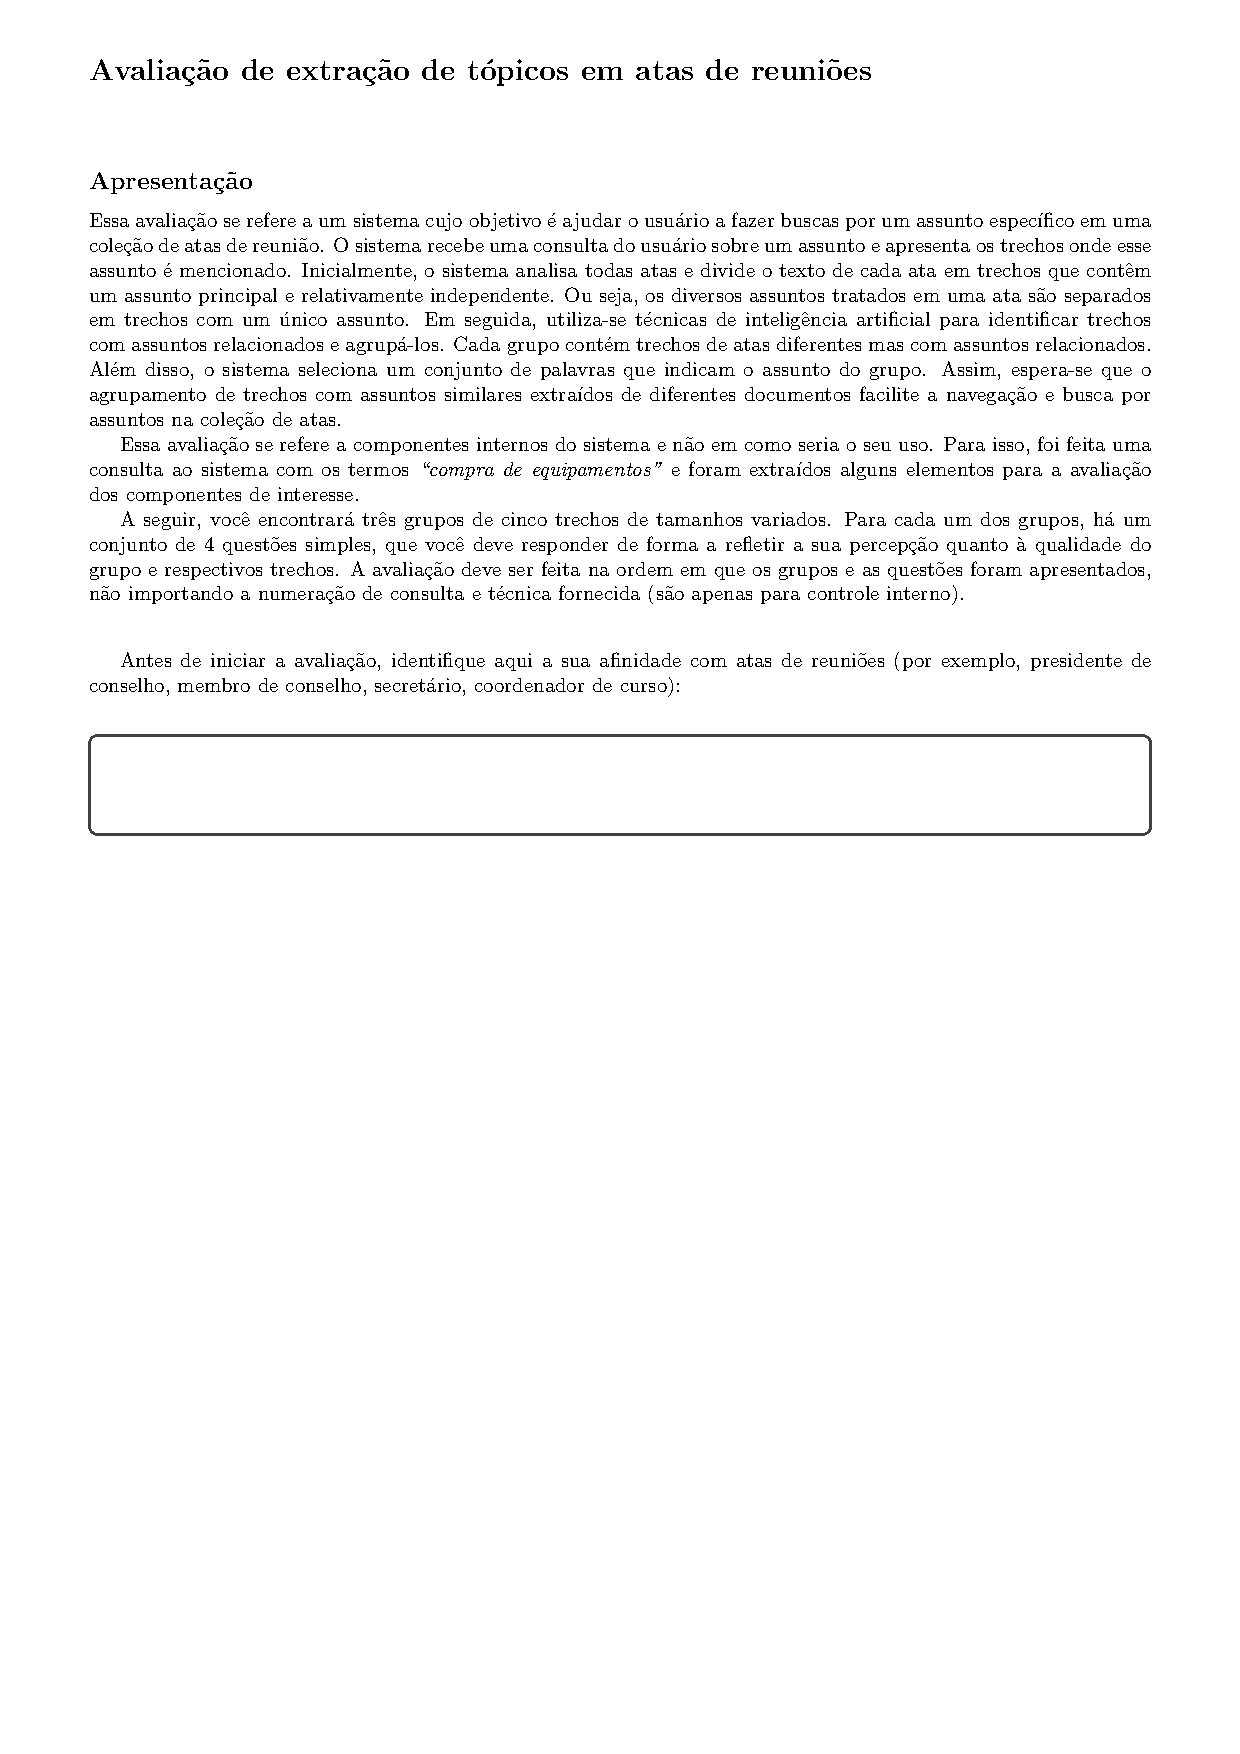
\includegraphics[trim={ 0 60 0 66 },clip,page=1,width=0.8\textwidth]{anexos/avaliacao-sistema/avaliacao-sistema.pdf}

\begin{figure}[h!]
\center
	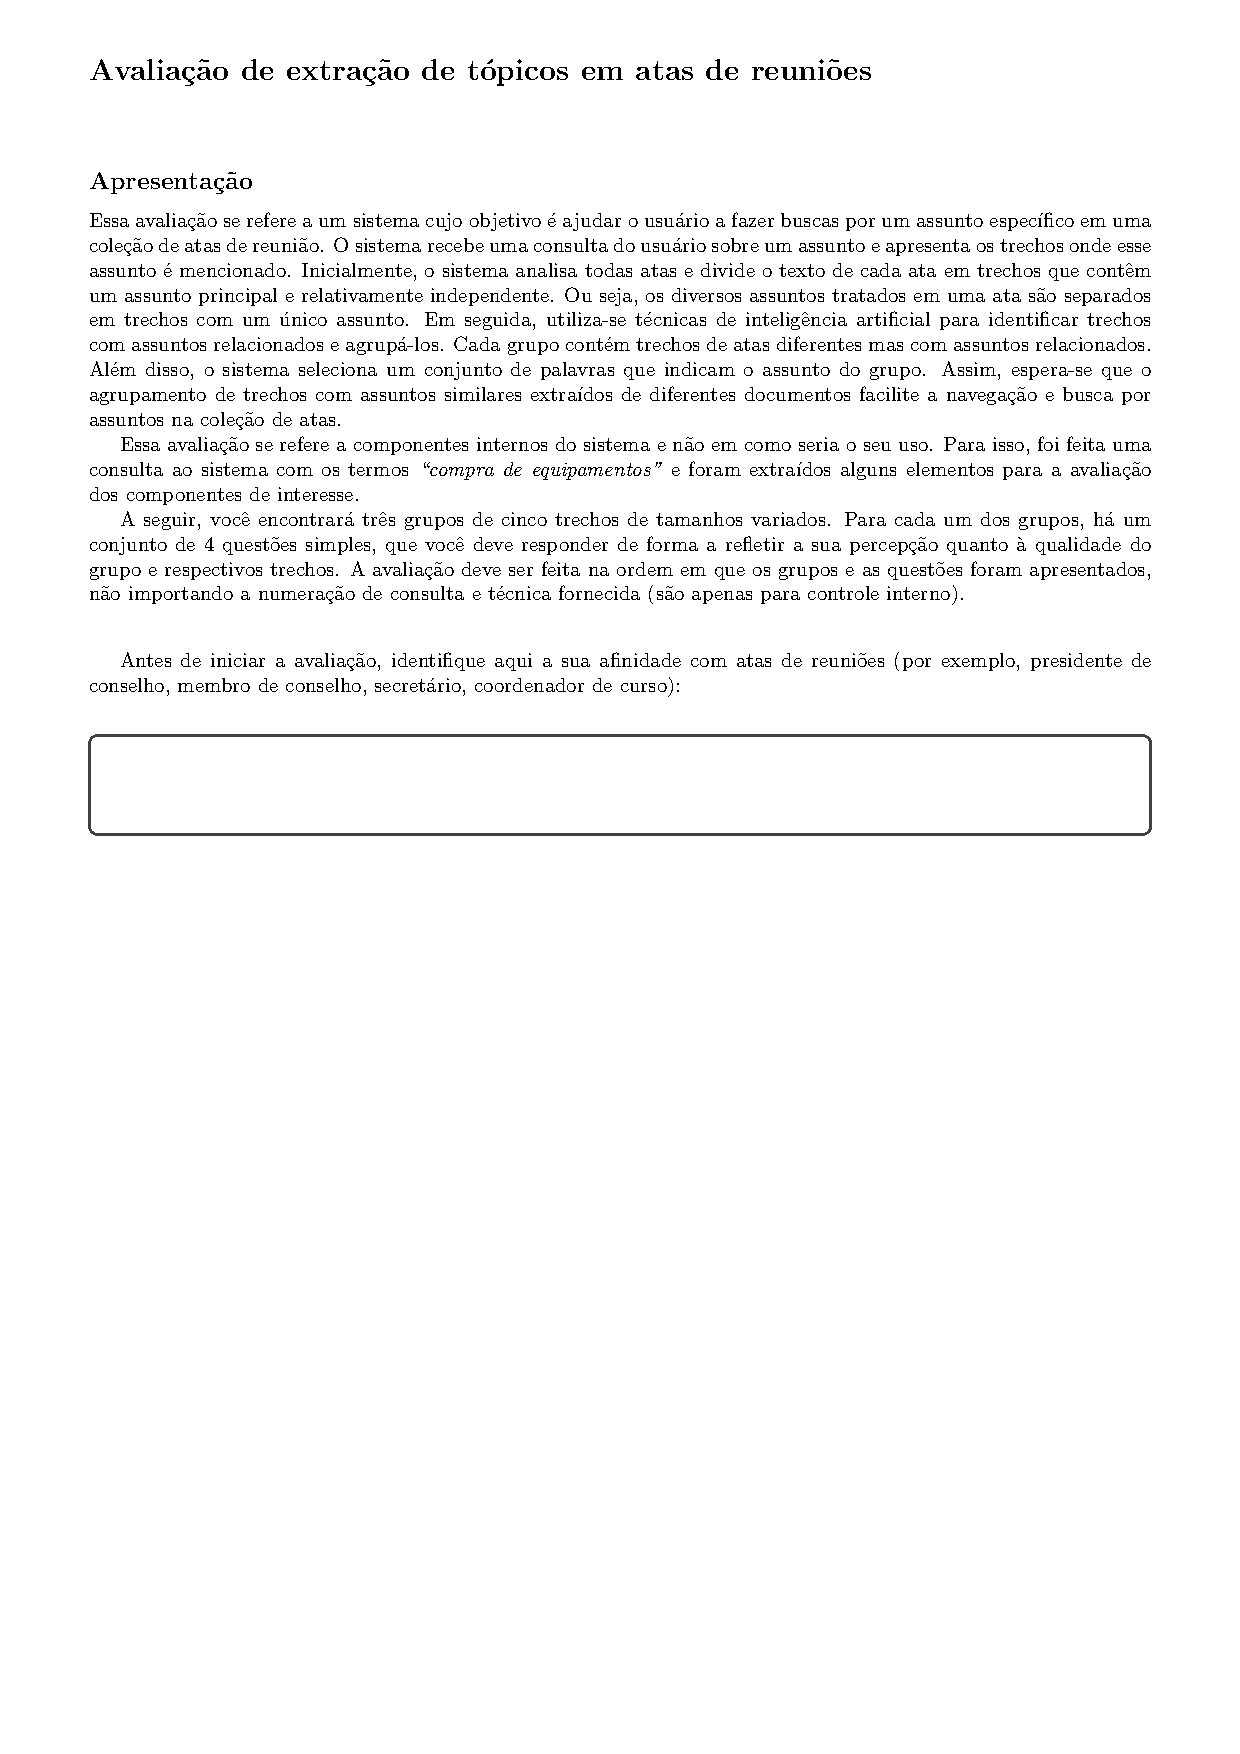
\includegraphics[trim={ 40 0 0 0 }, trim={ 0 60 0 66 }, page=1,width=1.1\textwidth]{anexos/avaliacao-sistema/avaliacao-sistema.pdf}
\end{figure}


\begin{figure}[h!]
\center
	\includegraphics[trim={ 40 0 0 0 }, page=2,width=1.1\textwidth]{anexos/avaliacao-sistema/avaliacao-sistema.pdf}
\end{figure}



\begin{figure}[h!]
\center
	\includegraphics[trim={ 40 0 0 0 }, page=3,width=1.1\textwidth]{anexos/avaliacao-sistema/avaliacao-sistema.pdf}
\end{figure}

\begin{figure}[h!]
\center
	\includegraphics[trim={ 40 0 0 0 }, page=4,width=1.1\textwidth]{anexos/avaliacao-sistema/avaliacao-sistema.pdf}
\end{figure}

\begin{figure}[h!]
\center
	\includegraphics[trim={ 40 0 0 0 }, page=5,width=1.1\textwidth]{anexos/avaliacao-sistema/avaliacao-sistema.pdf}
\end{figure}

\begin{figure}[h!]
\center
	\includegraphics[trim={ 40 0 0 0 }, page=6,width=1.1\textwidth]{anexos/avaliacao-sistema/avaliacao-sistema.pdf}
\end{figure}



\begin{figure}[h!]
\center
	\includegraphics[trim={ 40 0 0 0 }, page=7,width=1.1\textwidth]{anexos/avaliacao-sistema/avaliacao-sistema.pdf}
\end{figure}




\begin{figure}[h!]
\center
	\includegraphics[trim={ 40 0 0 0 }, page=8,width=1.1\textwidth]{anexos/avaliacao-sistema/avaliacao-sistema.pdf}
\end{figure}




\begin{figure}[h!]
\center
	\includegraphics[trim={ 40 0 0 0 }, page=9,width=1.1\textwidth]{anexos/avaliacao-sistema/avaliacao-sistema.pdf}
\end{figure}



\begin{figure}[h!]
\center
	\includegraphics[trim={ 40 0 0 0 }, page=9,width=1.1\textwidth]{anexos/avaliacao-sistema/avaliacao-sistema.pdf}
\end{figure}

\begin{figure}[h!]
\center
	\includegraphics[trim={ 40 0 0 0 }, page=10,width=1.1\textwidth]{anexos/avaliacao-sistema/avaliacao-sistema.pdf}
\end{figure}

\begin{figure}[h!]
\center
	\includegraphics[trim={ 40 0 0 0 }, page=12,width=1.1\textwidth]{anexos/avaliacao-sistema/avaliacao-sistema.pdf}
\end{figure}

\begin{figure}[h!]
\center
	\includegraphics[trim={ 40 0 0 0 }, page=13,width=1.1\textwidth]{anexos/avaliacao-sistema/avaliacao-sistema.pdf}
\end{figure}

\begin{figure}[h!]
\center
	\includegraphics[trim={ 40 0 0 0 }, page=14,width=1.1\textwidth]{anexos/avaliacao-sistema/avaliacao-sistema.pdf}
\end{figure}



\chapter{ Distribuição dos Tópicos obtidos pelos extratores}\label{apendice3}




Nesse apêndice podem ser observadas as distribuições dos tópicos obtidos pelos extratores.
Os extratores K-Means, LDA e PLSA foram executados com o \textit{corpus} estudado nesse trabalho, do qual extraiu-se 70 tópicos com 5 descritores por tópico. Os tópicos extraídos são representados por seus descritores e as colunas marcadas com \#Seg indicam a quantidade de segmentos atribuída a um tópico.
Os dados podem ajudar a entender a distribuição dos assuntos registrados na coleção de documentos, conforme discutido no Capítulo~\ref{cap3}.

\begin{landscape}% Landscape page

	% 
\begin{table}[!h]
	\tiny
	\centering
	\begin{tabular}{|l|c||l|c||l|c|} 
		\hline


		\multicolumn{2}{|c||}{ \textbf{K-Means} } & \multicolumn{2}{c||}{ \textbf{LDA} } & \multicolumn{2}{c|}{ \textbf{PLSA} } \\ \hline
		\textit{Descritores} & \textit{\#Seg} & \textit{Descritores} & \textit{\#Seg} & \textit{Descritores} & \textit{\#Seg} \\ \hline



   dia; realizada; chamada; estado; conselho;    &   116  &         disciplinas; cursadas; fichas; caracterização; aprovado;    &   107  &       docentes; presidente; dia; discente; téc;    &   76   \\ \hline
   informado; compra; ofício; pedido; processo;    &   106  &         colocar; deve; poderia; referentes; seriam;    &   94  &       disciplinas; álgebra; linear; geometria; analítica;    &   75  \\ \hline
   computação; conselho; aprovado; acordo; ficou;    &   102  &         docentes; presidente; técnica; dia; administrativo;    &   91  &       computação; acordo; levada; chefia; conselho;    &   62  \\ \hline
   docentes; técnica; administrativo; presidente; dia;    &   72  &         dia; aprovado; aprovação; ordem; anterior;    &   85  &       aprovado; aprovação; unanimidade; foram; ordinária;    &   57  \\ \hline
   representante; discente; presidente; secretária; turma;    &   55  &         representante; técnica; administrativo; secretária; discente;    &   79  &       representante; discente; piccoli; turma; pauta;    &   51  \\ \hline
   cursadas; conselho; coordenação; computação; presidente;    &   45  &         conselho; junto; assina; acordo; ficou;    &   69  &       técnica; administrativo; representante; secretária; discente;    &   45  \\ \hline
   aprovado; aprovação; atividades; relatórios; lido;    &   44  &         seguintes; chamada; conselho; data; ano;    &   67  &       comunicação; presidência; informado; verba; ocorrerá;    &   38  \\ \hline
   computação; cursadas; conselho; título; discente;    &   37  &         presença; realizada; cidade; leme; métricas;    &   55  &       bacharelado; coordenação; cursadas; encerrada; acordo;    &   37  \\ \hline
   disciplinas; cursadas; libras; conselho; aprovado;    &   36  &         presidência; comunicação; informado; iniciou; agradeceu;    &   54  &       afastamento; aprovado; aprovação; apresentar; referentes;    &   35  \\ \hline
   professores; colocar; regras; seriam; sugeriu;    &   30  &         atividades; extensão; relatórios; aprovado; aprovação;    &   52  &       dia; ordem; anterior; informado; pedido;    &   35  \\ \hline
   pedido; informado; substituí; laboratório; disciplinas;    &   30  &         havendo; lavra; iniciou; trabalho; trata;    &   46  &       discente; representante; lúcio; presidente; seki;    &   34  \\ \hline
   aprovado; trocar; pedido; analisada; fichas;    &   28  &         verba; compra; pagamento; valor; material;    &   46  &       informado; compra; ofício; material; verba;    &   34  \\ \hline
   dia; ordem; concurso; dezembro; foram;    &   27  &         afastamento; aprovado; aprovação; relatórios; lido;    &   44  &       presidente; presentes; lavra; havendo; comunicou;    &   30  \\ \hline
   representante; administrativo; técnica; discente; secretário;    &   26  &         coordenação; deliberar; restrito; junto; assina;    &   39  &       dia; seguintes; presidente; realizada; participante;    &   28  \\ \hline
   afastamento; aprovado; referentes; relatórios; final;    &   26  &         discente; representante; presidente; lúcio; seki;    &   34  &       relatórios; aprovado; lido; aprovação; atividades;    &   28  \\ \hline
   extensão; atividades; coordenadores; programa; relatórios;    &   25  &         computador; tópicos; disciplinas; software; dados;    &   30  &       dia; realizada; gestão; tecnologia; centrada;    &   27  \\ \hline
   compra; informado; verba; tem; valor;    &   23  &         disciplinas; calculada; diferentes; introdução; algoritmos;    &   27  &       dcomp; semestre; calendário; anexo; data;    &   26  \\ \hline
   aprovado; conselho; orientada; pedido; meses;    &   22  &         gestão; conhecimento; conselho; computação; sistema;    &   26  &       título; suplente; computação; iniciou; havendo;    &   25  \\ \hline
   dia; ordem; aprovação; anterior; aprovado;    &   22  &         processo; semestre; seletivo; resultado; ingresso;    &   26  &       fichas; caracterização; obrigatório; disciplinas; computação;    &   20  \\ \hline
   presidente; secretária; associado; chistine; dia;    &   20  &         laboratório; máquina; técnica; pedido; manutenção;    &   22  &       chamada; terceiro; dia; segunda; estado;    &   19  \\ \hline
   unanimidade; aprovado; conselho; ordinária; apreciação;    &   19  &         aprovado; defesa; pedido; dissertação; orientada;    &   17  &       dia; realizada; estado; presentes; cidade;    &   17  \\ \hline
   foram; aprovado; lido; relatórios; documentos;    &   19  &         conselho; cursadas; sala; computação; ano;    &   16  &       cursadas; disciplinas; coordenação; optativas; conselho;    &   17  \\ \hline
   comunicação; presidência; presidente; conselho; computação;    &   18  &         concurso; dados; bancos; vaga; comunicação;    &   15  &       explicou; enviar; aprovação; trazido; pauta;    &   17  \\ \hline
   processo; seletivo; semestre; resultado; aprovado;    &   18  &         pauta; inclusão; pedido; aceita; suplente;    &   14  &       extensão; atividades; coordenadores; aprovado; proposta;    &   17  \\ \hline
   secretária; representante; presentes; técnica; administrativo;    &   17  &         condicionado; informado; compra; faltando; aparelhos;    &   13  &       computação; cursadas; conselho; representante; discente;    &   16  \\ \hline
   fichas; caracterização; disciplinas; aprovação; aprovado;    &   16  &         discussão; decidido; regras; colocar; seriam;    &   12  &       computador; sistema; software; disciplinas; engenharia;    &   16  \\ \hline
   aprovação; aprovado; política; atas; anterior;    &   16  &         próxima; trazido; tomadas; informado; trouxe;    &   12  &       atividades; extensão; processo; edital; coordenadores;    &   16  \\ \hline
   computação; teoria; paralela; tópicos; tutoria;    &   13  &         aprovado; aprovação; referentes; vista; política;    &   10  &       pedido; deve; informado; realizada; aulas;    &   16  \\ \hline
   candidatos; concurso; lista; divulgação; bolsa;    &   12  &         pedido; atendida; compra; professores; informado;    &   10  &       cursadas; recurso; dcomp; laboratório; contar;    &   15  \\ \hline
   semestre; conceito; fronteiras; manutenção; esquema;    &   12  &         implantação; serviços; horária; prestados; unidades;    &   10  &       orientada; prazo; meses; defesa; final;    &   15  \\ \hline
   aprovação; realizada; laboratório; correções; trazido;    &   11  &         votação; votaram; equipe; verificaram; opção;    &   9  &       dia; conceito; laboratório; chamada; primeiro;    &   14  \\ \hline
   redigida; lavra; presidente; trabalho; coube;    &   10  &         foram; material; estado; detalhes; conseguiu;    &   8  &       extensão; programa; coordenadores; tecnologia; semana;    &   14  \\ \hline
   deve; normalizado; assunto; estudos; desejamos;    &   10  &         foram; conselho; aprovado; realizada; referendum;    &   7  &       projeto; comissão; esclarecido; faltando; bolsa;    &   13  \\ \hline
   havendo; legal; número; iniciou; introdução;    &   10  &         site; informado; dcomp; laboratório; ficou;    &   7  &       ficou; novo; colocar; regimento; votação;    &   13  \\ \hline
   realizada; pagamento; apresentação; the; learning;    &   9  &         deve; laboratório; aprovado; controlados; manter;    &   6  &       planos; ensino; foram; disciplinas; adequação;    &   13  \\ \hline
   aprovação; anterior; máquina; aprendizado; atas;    &   9  &         learning; the; and; artigo; apresentação;    &   6  &       provas; candidatos; presidente; solicitada; concurso;    &   12  \\ \hline
   pauta; inclusão; pedido; aceita; conselho;    &   8  &         projeto; extensão; mudanças; atividades; desenvolvimento;    &   6  &       professores; cursadas; justificativa; computação; ausência;    &   12  \\ \hline
   presentes; lavra; junto; assina; castilho;    &   8  &         aprovado; dcomp; proposta; foram; processo;    &   3  &       área; concurso; problemas; enviar; cursadas;    &   12  \\ \hline
   presidente; docentes; dia; cancelamento; governo;    &   7  &         sugeriu; mail; poderia; enviar; contato;    &   2  &       valor; compra; empenho; auxílio; verba;    &   12  \\ \hline
   ausência; justificativa; solicitação; períodos; afastamento;    &   7  &         informado; aprovado; comissão; eleição; deve;    &   1  &       graduação; pós; min; dia; realizada;    &   11  \\ \hline
   técnica; administrativo; docentes; dia; eihara;    &   7  &         informado; aprovado; dia; deve; substituí;    &   1  &       vaga; transferência; foram; informática; cursadas;    &   11  \\ \hline
   presidência; comunicações; iniciou; comunicação; presidente;    &   6  &         aprovado; informática; informado; dia; dcomp;    &   1  &       bancos; dados; aprovado; estrutura; proposta;    &   11  \\ \hline
   comunicou; comunicação; conselho; presidente; presentes;    &   6  &         deve; lista; informado; conselho; aprovado;    &   1  &       demanda; compra; pedido; verba; professores;    &   10  \\ \hline
   dados; bancos; ccs; software; engenharia;    &   6  &         informado; deve; aprovado; dia; conselho;    &   1  &       verba; cursadas; pagamento; disciplinas; calculada;    &   10  \\ \hline
   informática; sociedade; docentes; ética; casadei;    &   6  &         deve; informática; conselho; informado; aprovado;    &   1  &       laboratório; manutenção; suplente; trocar; cabo;    &   10  \\ \hline
   estudos; liberados; instalação; apuração; eleição;    &   6  &         conselho; informado; dia; aprovado; ordem;    &   1  &       área; criação; conselho; projeto; suplente;    &   9  \\ \hline
   processo; participação; ficou; imagens; sinais;    &   6  &         conselho; dia; aprovado; informado; próxima;    &   1  &       laboratório; disciplinas; votaram; proposta; créditos;    &   9  \\ \hline
   extensão; atividades; coordenadores; mitsuru; lúcio;    &   6  &         informática; conselho; informado; dcomp; comissão;    &   1  &       disciplinas; cursadas; oferta; horário; oferecida;    &   9  \\ \hline
   presidência; informado; comunicação; iniciou; presença;    &   5  &         aprovado; deve; informado; conselho; comissão;    &   1  &       manutenção; informado; laboratório; conseguiu; evento;    &   9  \\ \hline
   votaram; conselho; favor; eleitos; relação;    &   5  &         informática; informado; conselho; aprovado; deve;    &   1  &       colocar; lecionar; disciplinas; fechaduras; realizada;    &   9  \\ \hline
   iniciou; poderia; gestante; encontrados; compareceram;    &   5  &         conselho; informado; aprovado; final; deve;    &   1  &       laboratório; conselho; colocar; disciplinas; nus;    &   9  \\ \hline
   unidades; positivo; leitura; proposta; alterações;    &   5  &         aprovado; conselho; informado; recurso; eleição;    &   1  &       estágio; cursadas; atividades; coordenação; complementares;    &   8  \\ \hline
   discussão; dcomp; normalizado; material; item;    &   5  &         deve; dia; bolsa; lista; próxima;    &   1  &       colocar; diz; esclarecido; professores; seriam;    &   8  \\ \hline
   havendo; trata; deus; encerrada; presentes;    &   5  &         informado; conselho; deve; eleição; aprovado;    &   1  &       conselho; computação; cursadas; reuniu; ordinária;    &   7  \\ \hline
   votação; entrou; solicitada; transferência; responsável;    &   5  &         aprovado; unanimidade; conselho; informado; dia;    &   1  &       candidatos; dados; concurso; palestra; área;    &   6  \\ \hline
   recurso; foram; adequação; encaminhada; levantadas;    &   5  &         próxima; informado; aprovado; conselho; proposta;    &   1  &       sala; informado; orçamento; valor; site;    &   6  \\ \hline
   avaliação; extensão; discussão; projeto; ficou;    &   5  &         aprovado; deve; dcomp; informado; unanimidade;    &   1  &       proposta; colocar; copq; pesquisa; terá;    &   6  \\ \hline
   associado; presidente; chistine; existam; discente;    &   4  &         conselho; informado; dia; pedido; deve;    &   1  &       cursadas; existam; pedido; ofício; laboratório;    &   6  \\ \hline
   persianas; pedido; foram; cota; procurando;    &   4  &         palestra; apoio; sustentabilidade; informática; documentos;    &   1  &       bolsa; cursadas; distribuição; realizada; disciplinas;    &   6  \\ \hline
   estágio; apresentação; secretário; lúcio; eduardo;    &   4  &         próxima; conselho; discussão; informado; proposta;    &   1  &       disciplinas; tem; colocar; acadêmico; seriam;    &   6  \\ \hline
   gestão; ambiental; noções; vaga; distribuídos;    &   4  &         informado; conselho; dia; deve; aprovado;    &   1  &       presidente; discussão; cursadas; acrescentou; professores;    &   5  \\ \hline
   piccoli; ausência; justificativa; cancelamento; governo;    &   4  &         implantação; horária; serviços; dia; prestados;    &   1  &       junto; assina; participante; lavra; estado;    &   5  \\ \hline
   calendário; apresentar; dcomp; dia; ordinária;    &   4  &         informado; deve; transferência; informática; dcomp;    &   1  &       colocar; verba; poderia; informado; terá;    &   5  \\ \hline
   sistema; técnica; relatórios; publicação; proposta;    &   3  &         aprovado; dia; conselho; deve; informado;    &   1  &       chefia; seriam; criar; conselho; conflito;    &   5  \\ \hline
   gasto; verba; custeio; veio; lista;    &   3  &         participação; evento; palestra; sustentabilidade; partir;    &   1  &       capacitação; afastamento; regras; docentes; discussão;    &   5  \\ \hline
   sistema; operacionais; ccs; gestão; planos;    &   3  &         comissão; eleição; aprovado; conselho; dcomp;    &   1  &       seriam; edital; colocar; item; terá;    &   5  \\ \hline
   semana; estudos; perfil; ficou; apresentar;    &   2  &         deve; dia; conselho; aprovado; informado;    &   1  &       cursadas; proposta; atividades; esclarecido; colocar;    &   4  \\ \hline
   professores; férias; resposta; unanimidade; questões;    &   2  &         conselho; informado; substituição; aprovado; deve;    &   1  &       ano; dia; interessados; realizada; mês;    &   3  \\ \hline
   moraes; assunto; trata; breve; discussão;    &   2  &         dia; deve; conselho; docentes; aprovado;    &   1  &       projeto; foram; pesos; pedido; texto;    &   3  \\ \hline
   fapesp; rti; cocccs; ordinária; extraordinária;    &   2  &         conselho; pedido; dia; informática; informado;    &   1  &       disciplinas; requisitos; pré; professores; colocar;    &   1  \\ \hline










	\end{tabular}
	\caption{Tópicos obtidos com os extratores \textit{K-Means}, \textit{LDA} e \textit{PLSA}. 
As linhas representam os tópicos, para os quais são mostrados 5 descritores e a quantidade de segmentos atribuídos.
	% Para cada extrator é mostrado 5 descritores e a quantidade de documentos atribuídos a cada tópico.
}
	\label{tab:resumo-resultados}
\end{table}

	






\begin{figure}[h]
\center
	% \includegraphics[trim={ 40 0 0 0 }, trim={ 0 60 0 66 }, page=1,width=1.1\textwidth]{anexos/tabelas/distribuicao-topicos/distribuicao-topicos.pdf}
	\includegraphics[trim={ 40 600 200 0 }, page=1,width=1.2\textwidth]{anexos/tabelas/distribuicao-topicos/distribuicao-topicos.pdf}
\end{figure}





\begin{table}[b]
	\caption{Distribuições dos tópicos obtidos pelos extratores.}
\end{table}




\end{landscape}



\end{apendicesenv}
% ---

% ----------------------------------------------------------
% Anexos
% ----------------------------------------------------------

% ---
% Inicia os anexos
% ---
\begin{anexosenv}

% \chapter{Título}\label{anexo1}

Texto ou documento não elaborado pelo autor, que serve de fundamentação, comprovação e ilustração.

\end{anexosenv}
% --- 

%---------------------------------------------------------------------
% INDICE REMISSIVO
%---------------------------------------------------------------------
% \phantompart
% \printindex
%---------------------------------------------------------------------

\end{document}
